\documentclass{article}
\usepackage{graphicx}
\usepackage{wrapfig}
\usepackage{subcaption}
\usepackage[margin=1in]{geometry}
\usepackage{amsmath} % or simply amstext
\usepackage{siunitx}
\usepackage{booktabs}
\usepackage[export]{adjustbox}
\newcommand{\angstrom}{\textup{\AA}}
\newcommand{\colormap}{jet}  % colorbar to use
\usepackage{cleveref}
\usepackage{booktabs}
\usepackage{gensymb}
\usepackage{float}
\title{Understanding the nanoscale structure of hexagonal phase lyotropic liquid crystal membranes}
\author{Benjamin J. Coscia \and Douglas L. Gin \and Richard D. Noble \and Joe Yelk \and Matthew Glaser \and Xunda Feng \and Michael R. Shirts} 
\begin{document}
  \bibliographystyle{ieeetr}
  \graphicspath{{./figures/}}
  \maketitle
  \section*{Introduction}
  
  Nanostructured membrane materials have become increasingly popular for 
  aqueous separations applications such as desalination and biorefinement
  because they offer the ability to control membrane architecture at the
  atomic scale allowing the design of solute-specific separation membranes. \cite{humplik_nanostructured_2011}
  \begin{itemize}
    \item Most membrane-based aqueous separations of small molecules can 
    be achieved using reverse osmosis (RO) or nanofiltration (NF) \cite{van_der_bruggen_review_2003}
  \end{itemize}
  
  While RO and NF have seen many advances in the past few decades, they 
  are far from perfect separation technologies.
  \begin{itemize}
    \item \textit{RO membranes}
    \item Inconsistent performance : Current state-of-the-art RO membranes are unstructured with
    tortuous and polydisperse diffusion pathways which leads to 
    inconsistent performance \cite{song_nano_2011}
    \item High energy requirements : Necessarily high feed pressures 
    drive up energy requirements which strains developing regions and
    contributes strongly to CO\textsubscript{2} emissions. \cite{mcginnis_global_2008}
    \item Separation based on differences in solubility and diffusivity:
%MRS2: couldn't you argue that the fact that they diffuse and dissolve at different rates means that it makes it possible to design targeted separations?
%BJC: right, I say something like that in the sentence following this one. It would be more challenging to design a targeted separation 
% especially if the feed is complex
    Moreover, designing RO membranes to achieve targeted separations of 
    specific solutes in a complex feed solution is nearly impossible because various solutes dissolve
    into and diffuse through the polymer matrix at different rates. \cite{wijmans_solution-diffusion_1995}
    \item With optimization, one can exploit these differences to create a functional
    selective barrier.
    \item \textit{NF membranes}
    \item NF was introduced as an intermediate between RO and ultrafiltration,
    having the ability to separate organic matter and salts on the order of 
    one nanometer in size.
%MRS2: is ``well-defined'' the right word if there is a ``pore size distribution''?
%BJC: By well-defined, I'm thinking of cylinders versus polymer matrix. One is definitely more
% defined than the other. What is the right word for that? unambiguous? explicit?
%MRS3: hmm.  Maybe look and see what other people call them when describing NF membranes.
    \item Larger and well-defined pores drive down energy requirements while
    still affording separation of solutes as small as ions to some degree \cite{van_der_bruggen_review_2003}
    \item NF is often used as a precursor to reverse osmosis
    \item Unfortunately, NF membranes, like RO, possess a pore size 
    distribution which limits their ability to perform precise separations \cite{bowen_modelling_2002}
  \end{itemize}
  
  Nanostructured membranes can bypass many of the performance issues which
  plague traditional NF and RO membranes.
  \begin{itemize}
    \item Tune size and functionality of building blocks to control pore
    size and shape: One can accomplish targeted separations with high 
    selectivity by tuning shape, size and functionality of the molecular
    building blocks which form these materials. 
    \item As a result, solute rejecting pores can have their sizes tuned
    uniformly, resulting in strict size cut-offs.
    \item Entirely different mechanisms may govern transport in a given
    nanostructured material which can inspire novel separation techniques.
  \end{itemize}
  
  Development of nanostructured materials has been limited by the ability
  to synthesize and scale various fundamentally sound technologies.
  \begin{itemize}
    \item Graphene sheets are atomically thick which results in excellent
    permeability but defects during manufacturing severely impact 
    selectivity. \cite{cohen-tanugi_multilayer_2016}
    \item Molecular dynamics simulations of carbon nanotubes show
    promise \cite{humplik_nanostructured_2011} but synthetic techniques are 
    unable to achieve scalable alignment and pore monodispersity.\cite{hata_water-assisted_2004,maruyama_growth_2005}
    \item Zeolites have sub-nm pores with a narrow pore size 
    distribution and MD simulations exhibit complete rejection of solvated ions, \cite{murad_molecular_1998}
    however, experimental rejection was low and attributed to interstitial
    defects formed during membrane synthesis \cite{li_desalination_2004}
    \item There is a need for a scalable nanostructured membrane
  \end{itemize}
  
  Self assembling lyotropic liquid crystals (LLCs) are a suitable candidate for
  aqueous separation applications. 
  \begin{itemize}
    \item LLCs share the characteristic ability of nanostructured membrane
    materials to create highly ordered structures with the added benefits
    of low cost and synthetic techniques feasible for 
    large scale production \cite{feng_scalable_2014}
    \item Neat liquid crystal monomer forms the thermotropic, Col\textsubscript{h}
    phase. The presence of water results in the H\textsubscript{II} phase.
    \item In both cases, monomers assemble into mesophases made of hexagonally
    packed, uniform size, cylinders with hydrophilic groups oriented inward
    towards the pore center and hydrophobic groups facing outward.
    \item H\textsubscript{II} and Col\textsubscript{h} phase systems created by
    the monomer named Na-GA3C11 have been extensively studied experimentally \cite{smith_ordered_1997, %BJC: IUPAC chemical name here?
    zhou_supported_2005,resel_h2-phase_2000,feng_scalable_2014,feng_thin_2016}. 
  \end{itemize}
 
  Research into LLC membranes has been revived in recent years.
  \begin{itemize}
    \item During early stages of exploration, mesophases formed by Na-GA3C11 could not be macroscopically
    aligned, resulting in low flux membranes, and no clear route towards 
    scalable and economical filtration. 
    \item In 2014, Feng et al. showed that the mesophases could be aligned 
    using a magnetic field with subsequent crosslinking to lock the structure
    in place \cite{feng_scalable_2014}
    \item In 2016, Feng et al. showed that the same result could be obtained 
    using a technique termed soft confinement \cite{feng_thin_2016}.
  \end{itemize}
 
  % BJC: Not sure this figure needs to be in the paper. 
  %MRS2: good question.  It helps give people context, which is necessary to move forward.  Perhaps 
  %leave it in for now, though may need to get permission to reprint it.
  \begin{figure}
	\centering
	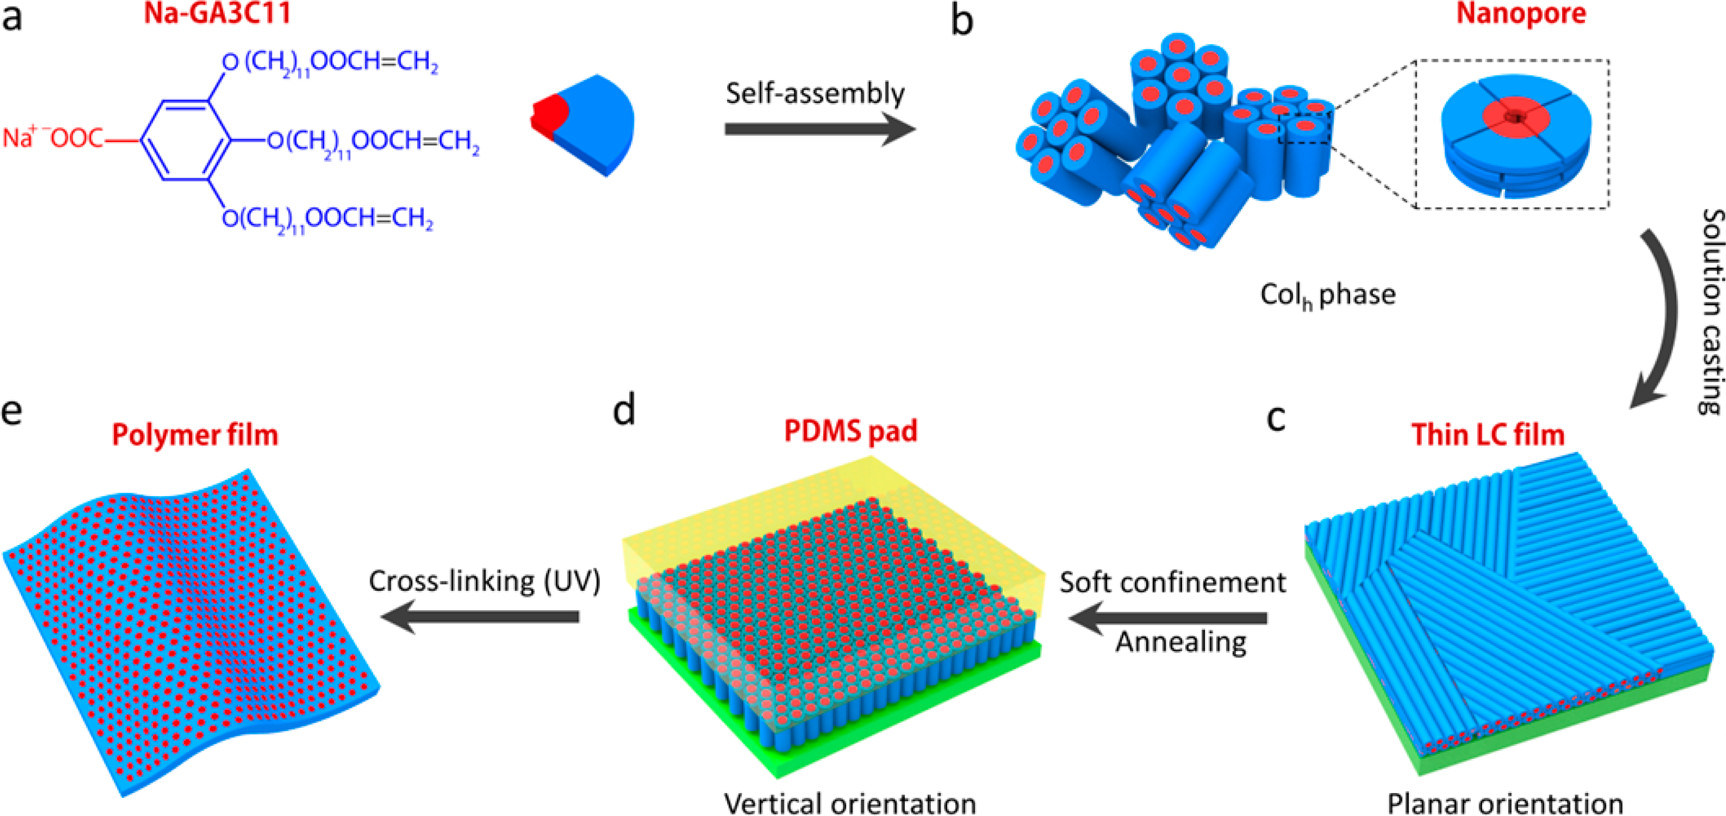
\includegraphics[width=\linewidth]{soft_confinement.png}
	\caption{The wedge shaped liquid crystal monomer (a) self assembles into 
	mesophases with hexagonally packed pores (b). The pores are made of 
	stacked monomer disks. A sub-micron-thick film is created by casting a 
	dilute solution of Na-GA3C11/THF solution onto a silicon substrate and 
	and allowing the solvent to evaporate. The thin film contains nanoporous 
	columns which lie parallel to the film plane. (d) When a soft PDMS pad is 
	imposed to the thin film, with subsequent thermal annealing, the columns
	align perpendicular to the film plane. (e) Photo-cross-linking of the
	aligned film creates a mechanically stable thin film with vertically 
	aligned nanopores}~\label{fig:soft}
  \end{figure}

  A molecular level understanding of LLC membrane structure, enabled by molecular
  dynamics simulations, will provide guidelines to reduce the large chemical space
  available to design monomers for creation of separation-specific membranes.
  \begin{itemize}
    \item Over the past 20 years, H\textsubscript{II} phase LLC membrane studies have been limited primarily
    to Na-GA3C11 with some characterization done after minor structural modifications
    \item Resel et al. varied the length of the monomer tails and the counterion used and 
    observed its affect on pore spacing \cite{resel_structural_2000}.
    \item Rejection studies show that this membrane can not perform separations of
    solutes less than 1.2 nm in diameter because the pores are too large \cite{zhou_supported_2005}.
    \item  We do not yet understand how to controllably reduce the effective pore size or 
    how to tune the chemical environment in the nanopores for effective water
    desalination or small organic molecule separations.
    \item It will be challenging to efficiently narrow down the large design space in 
    a laboratory setting without a robust model.
    \item The only source of predictive modeling for LLC systems have been macroscopic models 
    which likely do not adequately describe transport at these length scales. % BJC: Reference. I think it is just w.r.t. bicontinuous cubic
%MRS2: not quite sure of the phrasing here on next two points. Something more a long the lines of the choice of head group 
%may allow tuning rejection of solutes based on size?
%BJC: okay tried again
    \item The choice of head group may allow us to tune pore size for size exclusion driven separations
%MRS3: choice of counterion also affects size.  Counterion type probably doesn't affect Donnan potential that much IRCC, more the total amount of counterion.
    \item Choice of counterion may influence the establishment of a Donnan potential
    affecting the degree to which the membrane can exclude charged species.
    \item A good molecular model should incorporate a detailed picture of the nanoscopic pore 
    structure which will be crucial to understanding the role of monomer structure in 
    membrane design.
    \item Molecular dynamics simulations will provide the required level of detail
  \end{itemize}

  %BJC: Figure here showing previous level of detail compared to atomistic level of detail
  %MRS2: provenance of the atomistic figure could be explained better in the caption. It also looks disordered. Will eventually need a higher resolution figure for the previous understanding pore.
  %BJC: Okay. The picture here is of the "ordered pore" phase. It looks disorderd from this angle. I could use a different slice of the membrane to see if it looks any better
%MRS: if this is ordered, OK.  Maybe could try to rotate it a bit more towards the reader.
  \begin{figure}
  \centering
	\begin{subfigure}{0.45\linewidth}
		\centering
		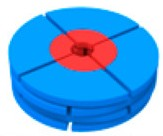
\includegraphics[width=\textwidth]{nanopore_undetailed.jpg}
		\caption{}~\label{fig:undetailed_pore}
	\end{subfigure}
	\begin{subfigure}{0.45\linewidth}
		\centering
		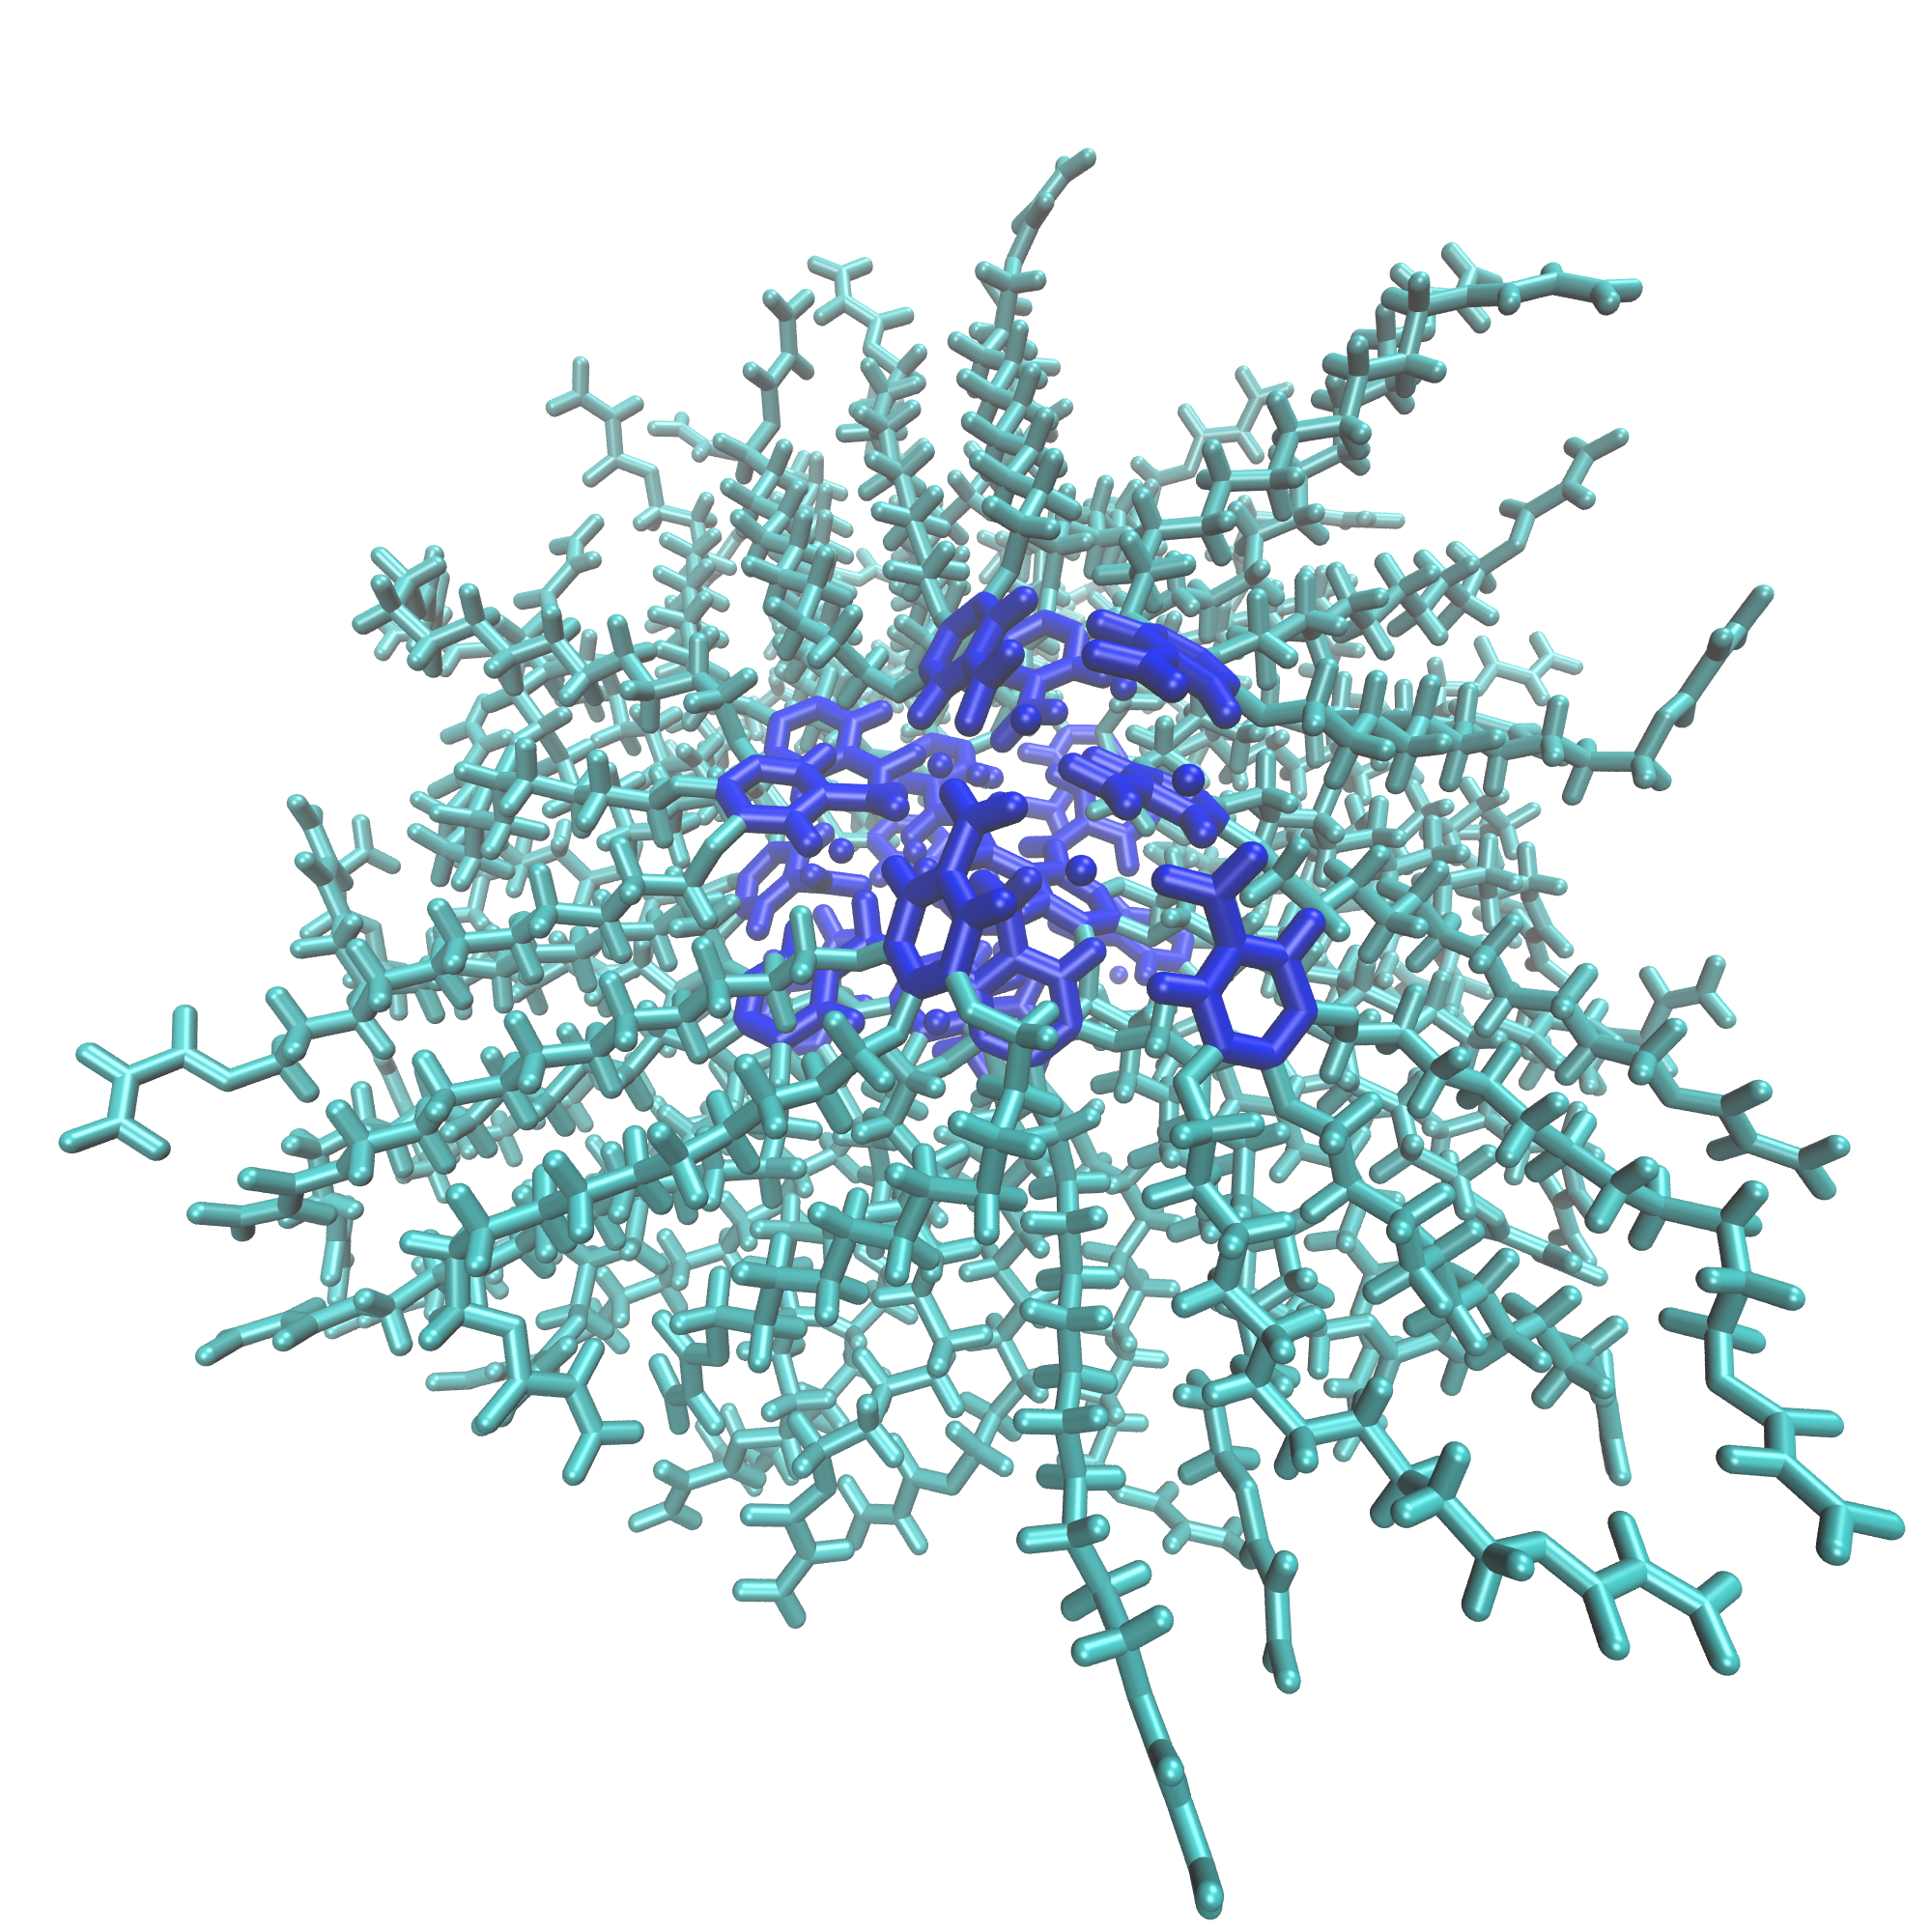
\includegraphics[width=\textwidth]{detailed_pore.png}
		\caption{}~\label{fig:detailed_pore}
	\end{subfigure}
  \caption{(a) Our previous understanding of the pore structure allows us to speculate
	   about separation behavior. (b) A detailed molecular model will allow us to
	   directly observe solute transport. Here, four stacked layers of 5 monomers
           are pictured atomistically. The hydrophilic region is in red and the 
	   hydrophoic region is colored blue.}~\label{fig:detail}
  \end{figure} 
	
  
  Our approach to constructing a general model will follow the development of a
  model of a specific LLC membrane with sufficient experimental characterization.
    \begin{itemize}
	    \item We have chosen to focus on assemblies formed by Na-GA3C11
	    \item We have also narrowed our scope to the development of 
	    a model of the Col\textsubscript{h} phase membrane.
	    \item Compared to the H\textsubscript{II} phase, the Col\textsubscript{h}
	    phase is a simpler starting point, due to the absence of water, and has
	    detailed experimental WAXS patterns useful for reconstructing structural data.  
    \end{itemize}

  Despite having structural data, there is still information which
  experiment cannot definitively answer. There are several key
  questions that we will investigate  
%MRS3: we can't ``answer'' for sure, since it's a model, and may omit things. Could put ``several key questions we will investigate'' or ``hope to provide evidence for or against'', or something like that.
which will be laid out and numbered
  in subsequent paragraphs.

%BJC: the following just seems like filler now that I've reorganized
%   A clear picture of the nanoscopic LLC membrane structure, gained by building 
%   a molecular model will provide evidence to answer existing and newly proposed
%   questions.
%     \begin{itemize}
%     \item Despite having structural data, there is still information which 
%     experiment cannot definitively answer
%     \end{itemize}

%MRS: break this down into more hierarchy - there are 11 separate points.  Can they be grouped at all for clearer understanding? elucidate what the aspects are we need a clearer picture. 
%BJC: I moved the logic for choice of monomer to system to model to a separate paragraph (above this). I then moved the other three things I talk about into their own paragraphs to keep the ideas separate (following paragraphs).
%MRS: since the questions we answer in the paper have a lot to do with the structure of the membranes, somewhere relatively early in the paper we need to lay out the facts that 1) these membranes could be really good (I think you do establish this) 2) we really would need to know the structure better to really do useful things with these, and 3) MD is a very helpful way to gain more information about the structure, because of the limited range of experiments we can do with these systems. That is the main rationale, and it should be made clear fairly early in the introduction.  Very important to make your story absolutely as clear as possible.
%BJC: I moved and edited a paragraph that was originally later on to be 2 above this one. I think it does a better job addressing points 2 and 3. And now it addresses those points earlier in the intro (as early as it could go where I think it still makes sense in context)

%BJC: How question (1) and (2) used to be ordered:
%
%  (1) Do monomers partition into and persist as defined monomer layers?
%  H\textsubscript{II} and Col\textsubscript{h} phase LC membrane pores are 
%  thought to be composed of monomer layers stacked on top of each other. 
%  \begin{itemize}
%  	\item Their existence is supported by experimental evidence of strong 
%	$\pi$-$\pi$ stacking interactions in the direction perpendicular to the
%	membrane plane.
%	\item $\pi$-$\pi$ stacking will only occur between monomer head groups which
%	leaves no description of what is happening in monomer tail region
%	\item It is possible that $\pi$-$\pi$ stacking occurs vertically 
%	with no order in reference to neighboring stacked columns of the same pore.  % BJC: not sure if this is actually true
%  \end{itemize}
%
%  (2) If layers do exist, how many monomers constitute a single layer?
%  There has been no definitive answer to the question in literature.
%  \begin{itemize}
%    \item A simple molecular simulation study of a similar molecule suggested
%    that there are 4 monomers in each layer. Their estimation is based on a
%    simulated system containing only 16 total monomers which likely does not sufficiently
%    model the chemical environment present in the real system.~\cite{zhu_methacrylated_2006}. 
%    \item A separate calculation based on the volume of the liquid crystal monomers proposes
%    that there are seven monomers in each layer~\cite{resel_structural_2000}. 
%    \item A molecular model orders of magnitude larger than any other reported atomistic 
%    liquid crystal membrane simulations has the best chance of directly answering this question.
%  \end{itemize}

%  Monomers in the Col\textsubscript{h} system are theorized to be partitioned
%  into stacked layers which form columnar pores. 
%BJC: commenting out :There has been no definitive answer in literature regarding the number of monomers in each layer. 
%MRS3: the intro to the list talks about only ``numbers of monomers in each layer'', whereas the list below talks about several questions relating to layers. Can you rephrase so it's more general? Maybe just take out that sentence above.
%We want to know 
%\begin{enumerate}
%\item If layers do exist, how many monomers constitute a single layer? \label{point:monomernum}
%  \begin{itemize}
%    \item A simple molecular simulation study of a similar molecule suggested
%    that there are 4 monomers in each layer. Their estimation is based on a
%    simulated system containing only 16 total monomers which likely does not sufficiently
%    model the chemical environment present in the real system.~\cite{zhu_methacrylated_2006}. 
%    \item A separate calculation based on the volume of the liquid crystal monomers proposes
%    that there are seven monomers in each layer~\cite{resel_structural_2000}. 
%    \item A molecular model orders of magnitude larger than any other reported atomistic 
%    liquid crystal membrane simulations has the best chance of directly answering this question.
%    \item We can directly change the layer composition and note its effect on membrane structure.
%  \end{itemize}
%
% \item Does our model support the existence of layers and if so, how well defined
%  are the layers? \label{point:layers}
%  \begin{itemize}
%       \item Experimentally, their existence is supported by evidence of strong 
%       $\pi$-$\pi$ stacking interactions in the direction perpendicular to the
%       membrane plane.
%       \item $\pi$-$\pi$ stacking will only occur between the aromatic monomer head groups which
%       leaves no description of what is happening in the monomer tail region
%       \item The tails may entangle isotropically while stacking order is maintained
%       among headgroups. 
%  \end{itemize}  
%  
%   \item How do monomers in each layer position themselves with respect to surrounding 
%   layers? \label{point:orientation}
%%     Even if we knew the number of monomers in each layer, we still would not know how 
%%     monomers in each layer are positioned with respect to other layers. 
%   \begin{itemize}
%      \item The $\pi$-$\pi$ stacking interactions may be a driving force of self assembly 
%      in this system\cite{gazit_possible_2002} %is thought to be $\pi$-$\pi$ stacking interactions between aromatic headgroups \cite{gazit_possible_2002}. 
%      \item Gas phase ab initio studies of benzene dimers have shown a clear energetic
%      advantage for parallel displaced and T-shaped $\pi$-$\pi$ stacking conformations versus a
%      sandwiched conformation ~\cite{sinnokrot_estimates_2002}.
%      \item Substituted benzene rings exhibit an even stronger $\pi$-$\pi$ stacking 
%      attraction which favors the parallel displaced configuration in all cases
%      except where the substitutions are extremely electron withdrawing
%      \cite{waller_hybrid_2006,ringer_effect_2006}.
%      \item We can use simulated X-ray diffration patterns to compare the two 
%      stacking configurations. 
%   \end{itemize}
%
%  \item Can the system exist in other metastable states or phases that are not
%  accessed during experiments? \label{point:metastable}
%  There remains the possibility that there is more than one metastable state 
%  associated with a given LLC system.
%  \begin{itemize}
%    \item Simulating a membrane atomistically will require many atoms which further
%    limits the timescales acessible with MD
%    \item It is reasonable to expect that we will generate configurations which 
%    are kinetically trapped in a metastable free energy basin
%    \item We must be able to identify which state is produced experimentally and 
%    why others are not.
%  \end{itemize}
%
%  \item What constitutes a pore and how well-defined are the pore regions? \label{point:poredefinition}
%  \begin{itemize}
%	\item The limited picture that experiment provides tells us that there are
%        hexagonally packed, hydrophilic regions where transport is likely to occur
%	\item One may instinctively assume that these regions are tube-like pathways
%	\item We will explore the composition of the pores and the partition
%	between the hydrophilic and hydrophobic regions. 
%  \end{itemize}
%
%  \item Is it necessary to include any water in order to appropriately model the 
%  Col\textsubscript{h} phase? \label{point:water}
%  \begin{itemize}
%	\item While the Col\textsubscript{h} phase is described as dry, it is 
%          %MRS3: ``possible'' -> likely, and give some explanations why we think likely? 
%	likely that small amounts of ambient water may be leached into the system.
%	\item The hydrogen bonding network formed by the water may play a role 
%        in structuring the pore.
%	\item We can use simulated X-ray diffraction patterns to see if there is
%        any meaningful structural difference between a "dry" and "wet" system
%  \end{itemize}
%  \end{enumerate}
%  
  %Once we have addressed all of the above questions, we must show that the 
  %developed molecular model is consistent with physical observations so that we
  %can rely on conclusions drawn about structural features characteristic of 
  %the system.
 
  %BJC4: Consolidation of points into 4 main questions to answer
  There are a number of structural questions we wish to answer in this article. We
  want to know:
  \begin{enumerate}
    \item What is the density of monomers that pack around each hydrophilic core? 
    \label{point:monomernum}
 	\begin{itemize}
 		\item Authors often describe this and similar systems as being made up of layers.
 		\item A simple molecular simulation study of a similar molecule suggested
	    that there are 4 monomers in each layer. Their estimation is based on a
	    simulated system containing only 16 total monomers which likely does not sufficiently
	    model the chemical environment present in the real system.~\cite{zhu_methacrylated_2006}. 
	    \item A separate calculation based on the volume of the liquid crystal monomers proposes
	    that there are seven monomers in each layer~\cite{resel_structural_2000}. 
 		\item We are careful to avoid the term 'layers' since a liquid crystalline system has,
 		by definition, long range order in 1 or 2 spatial dimensions and short range order in 	
 		the other dimensions.~\cite{chaikin_principles_1995}  % page 58
 		\item In the system we are studying, there are long-range 2D correlations in the 
 		hexagonal array of pores and short range correlations in the z-direction.
		\item We will use our atomistic molecular model to study how the system's structure is
		effected by the density of monomers surrounding each pore's hydrophilic core. 
	\end{itemize}
	\item What structural motif best matches experimental 2D WAXS patterns?\label{point:xrdmatch}
	\begin{itemize}
		\item On the short timescales accessible to MD, we observe distinct metastable 
		configurations which are dependent on starting configuration.
		\item We simulate XRD patterns of our system and compare them to experimental 2D WAXS 
		patterns so that we ensure our model creates a nanoscopic chemical environment maximally
		consistent with experiment within the constraints of our forcefield.
                %MRS5: suggestion
		%\item We are able to confirm and refute previous interpretations of the WAXS pattern.  
		\item We are able to confirm some previous interpretations of the WAXS pattern and refute others.  
	\end{itemize}
	\item What is the chemical composition of the pores?\label{point:composition}
	\begin{itemize}
		\item The limited picture that experiment provides tells us that there are
        hexagonally packed, hydrophilic regions where transport is likely to occur
		\item One may instinctively assume that these regions are tube-like pathways with 
		well-defined boundaries.
		\item We will explore the composition of the pores, the partition
		between the hydrophilic and hydrophobic regions, and its sensitivity to initial
		configuration. 
	\end{itemize}
    \item Is it necessary to include any water in order to appropriately model the 
    Col\textsubscript{h} phase? \label{point:water}
    \begin{itemize}
		\item While the Col\textsubscript{h} phase is described as dry, it is likely that small 
		amounts of ambient water may be leached into the system.
		\item The hydrogen bonding network formed by the water may play a role in structuring the
		pore.
		\item We can use simulated X-ray diffraction patterns to see if there is any meaningful 
		structural difference between a "dry" and "wet" system
    \end{itemize}
  \end{enumerate}

  In this study, we build a significantly more realistic atomistic model of LLC membranes
  than has ever previously been done, and explore what new structural information can be gained
  and what structure hypotheses are supported by this model.

  \begin{itemize}
    \item We validate the model using as much experimental information as possible.
    \item We are most interested in reproducing the conclusions about structure
    which have been made from X-ray diffraction (XRD) experiments and in matching ionic
    conductivity measurements~\cite{feng_thin_2016}.
  \end{itemize}

  We used experimental wide angle X-ray scattering (WAXS) data (produced as described
  in~\cite{feng_scalable_2014}) and small angle X-ray scattering (SAXS) data from~\cite{feng_thin_2016}
  to inform our choices of some initial structural parameters (Figure~\ref{fig:SWAXS}). We rely primarily
  on the 2D WAXS data since it encodes all structural details down to the sub-nm scale.
  \begin{itemize}
        \item There are five major features of interest present in the 2D experimental
        pattern shown in Figure~\ref{fig:WAXS}.
        \item The first is located at $q_z$ = 1.7 \angstrom$^{-1}$,
        corresponding to a real spacing of 3.7 \angstrom~. The reflection is
        attributed to $\pi$-$\pi$ stacking between aromatic rings in the direction
        perpendicular to the membrane plane, or z-axis \cite{feng_scalable_2014}. For simplicity, this
        reflection will be referred to as R-$\pi$.
        \item A weak intensity line is located at exactly half the $q_z$ value of
        R-$\pi$ ($q_z$ = 0.85 \angstrom$^-1$), corresponding to a
        real space periodic spacing of 7.4 \angstrom~. This reflection has been
        interpreted  as 2\textsubscript{1} helical ordering of aromatic rings
        along the z axis meaning if the positions of the aromatic rings can
        be traced by a helix, then for each turn in the helix, there should be
        two aromatic rings. For this reason it will be referred to as R-double.
        \item A third major reflection is marked by a low intensity ring located
        at r = 1.4 \angstrom$^-1$. The real space separation
        corresponds to 4.5 \angstrom~ which is characteristic of the average
        spacing between packed alkane chains. This reflection will be called R-alkanes.
        \item Within R-alkanes, are four spots of higher relative intensity which
        will be called R-spots. All are located $\approx 40$ degrees from the $q_z$ axis
        in their respective quadrants. In many liquid crystal systems this can be
        explained by the tilt angle of the alkane chains with respect to the xy plane. % BJC: References
        \item The final feature corresponds to the spacing and symmetry of
        the d\textsubscript{100} plane which can be related to the distance between
        pores. The feature, which will be called R-pores, is characterized by dots
        along $q_z$ = 0. The spacing between dots is indicative of the hexagonal
        symmetry of the packed pores. The same information at higher resolution is obtained using a SAXS
        setup. By radially integrating the 2D data one gets a 1D curve which is
        shown in Figure~\ref{fig:SAXS}.  % BJC: I also have 2D SAXS data
  \end{itemize}

  \begin{figure}
        \centering
        \begin{subfigure}[t]{0.43\linewidth}
                \centering
        %       \vspace{12mm}
                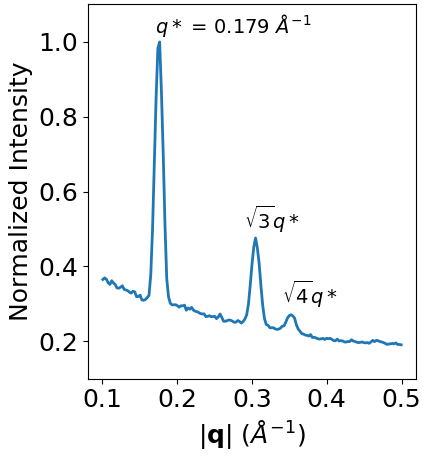
\includegraphics[width=\linewidth]{SAXS.png}
                \caption{}\label{fig:SAXS}
        \end{subfigure}
        \begin{subfigure}[t]{0.47\linewidth}
                \centering
                \raisebox{.2\textwidth}{%
                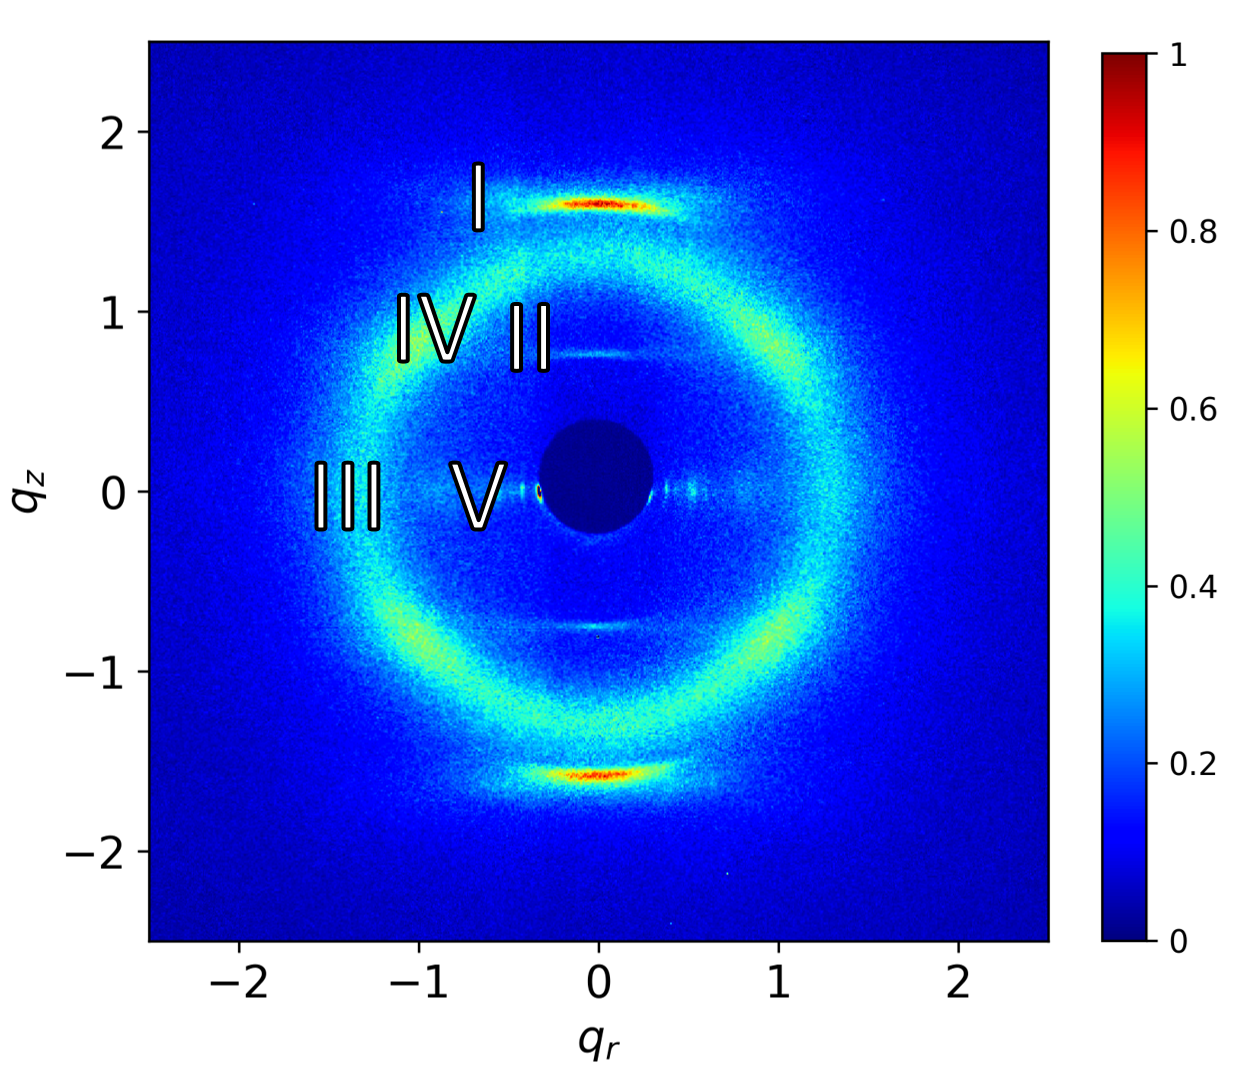
\includegraphics[width=\linewidth]{WAXS_annotated.png}
                }
                \caption{}\label{fig:WAXS}
        \end{subfigure}
        \caption{(a) 1D small angle X-ray scattering indicates hexagonal packing of
        pores as well as the spacing between pores (b) 2D wide angle X-ray scattering
        gives details about repeating features less than 1 nanometer apart}\label{fig:SWAXS}
        %MRS5: eventually will need to put the roman numerals with the names here in the caption. 
 \end{figure}

%    \begin{itemize}
%            \item We have compared simulated X-ray diffraction patterns to experiment in
%            order to match major features present in the 2D patterns.
%            \item We calculated ionic conductivity using two agreeing methods.
%            \item We examined the the influence of crosslinking on membrane structure.
%    \end{itemize}
%    \item The structure-building approach and analysis used in this paper can be readily extended
%    to the H\textsubscript{II} phase, other similar LC systems and ultimately to help design
%    real membranes.
%  \end{itemize}
  
  \section*{Methods}
 
  %BJC: The Methods sections has four main topics which will be separated by an appropriate header

  %%%%%%%%% Monomer Preparation %%%%%%%%%%%%%
 
  Liquid crystal monomers were parameterized using the Generalized AMBER Forcefield
  \cite{wang_development_2004} with the Antechamber package \cite{wang_automatic_2006}
  provided with AmberTools16 \cite{case_ambertools16_2016}. Atomic charges were
  assigned using the am1bccsym method of molcharge shipped with QUACPAC from Openeye % cite with webpage
  Scientific Software. All molecular dynamics simulations were run using Gromacs 2016  % This the version on Bridges
  \cite{bekker_gromacs:_1993,berendsen_gromacs:_1995,van_der_spoel_gromacs:_2005,hess_gromacs_2008}
  
  An ensemble of characteristic, low-energy vacuum monomer configurations
  were constructed by applying a simulated annealing process to a
  parameterized monomer.
  %MRS5: probably want to give more details in supporting information.
  \begin{itemize}
    \item Monomers were cooled from 1000K to 50K over 10 nanoseconds.
    \item A low energy configuration was randomly pulled from the trajectory
    and charges were reassigned with molcharge. 
    \item Using the new charges, the monomer system was annealed again and monomer
    configurations were pulled from the trajectory to be used for full
    system construction (Figure~\ref{fig:python}a).
  \end{itemize}

  %%%%%%%% UnitCell Preparation %%%%%%%%%%%%%

  The timescale for self assembly of monomers into the hexagonal phase is
  unknown and likely outside of a reasonable length for an atomistic
  simulation, calling for a more efficient way to build the system. 
  \begin{itemize}
    \item Previous work has shown a coarse grain model self assemble into
    the H\textsubscript{II} phase configuration in $\approx$ 1000 ns \cite{mondal_self-assembly_2013}.
    \item We attempted atomistic self-assembly by packing monomers into a box 
    using Packmol \cite{martinez_packmol:_2009}.
    \item Simulations of greater than 100 ns show no indicators of progress 
    towards an ordered system.  %BJC: include more details in supplment
    \item To bypass the slow self-assembly process, python scripts are used
    to assemble monomers into a structure close to one of a number of 
    hypothesized equilibrium configurations (Figure~\ref{fig:python}).
  \end{itemize}

  \begin{figure}
	\centering
	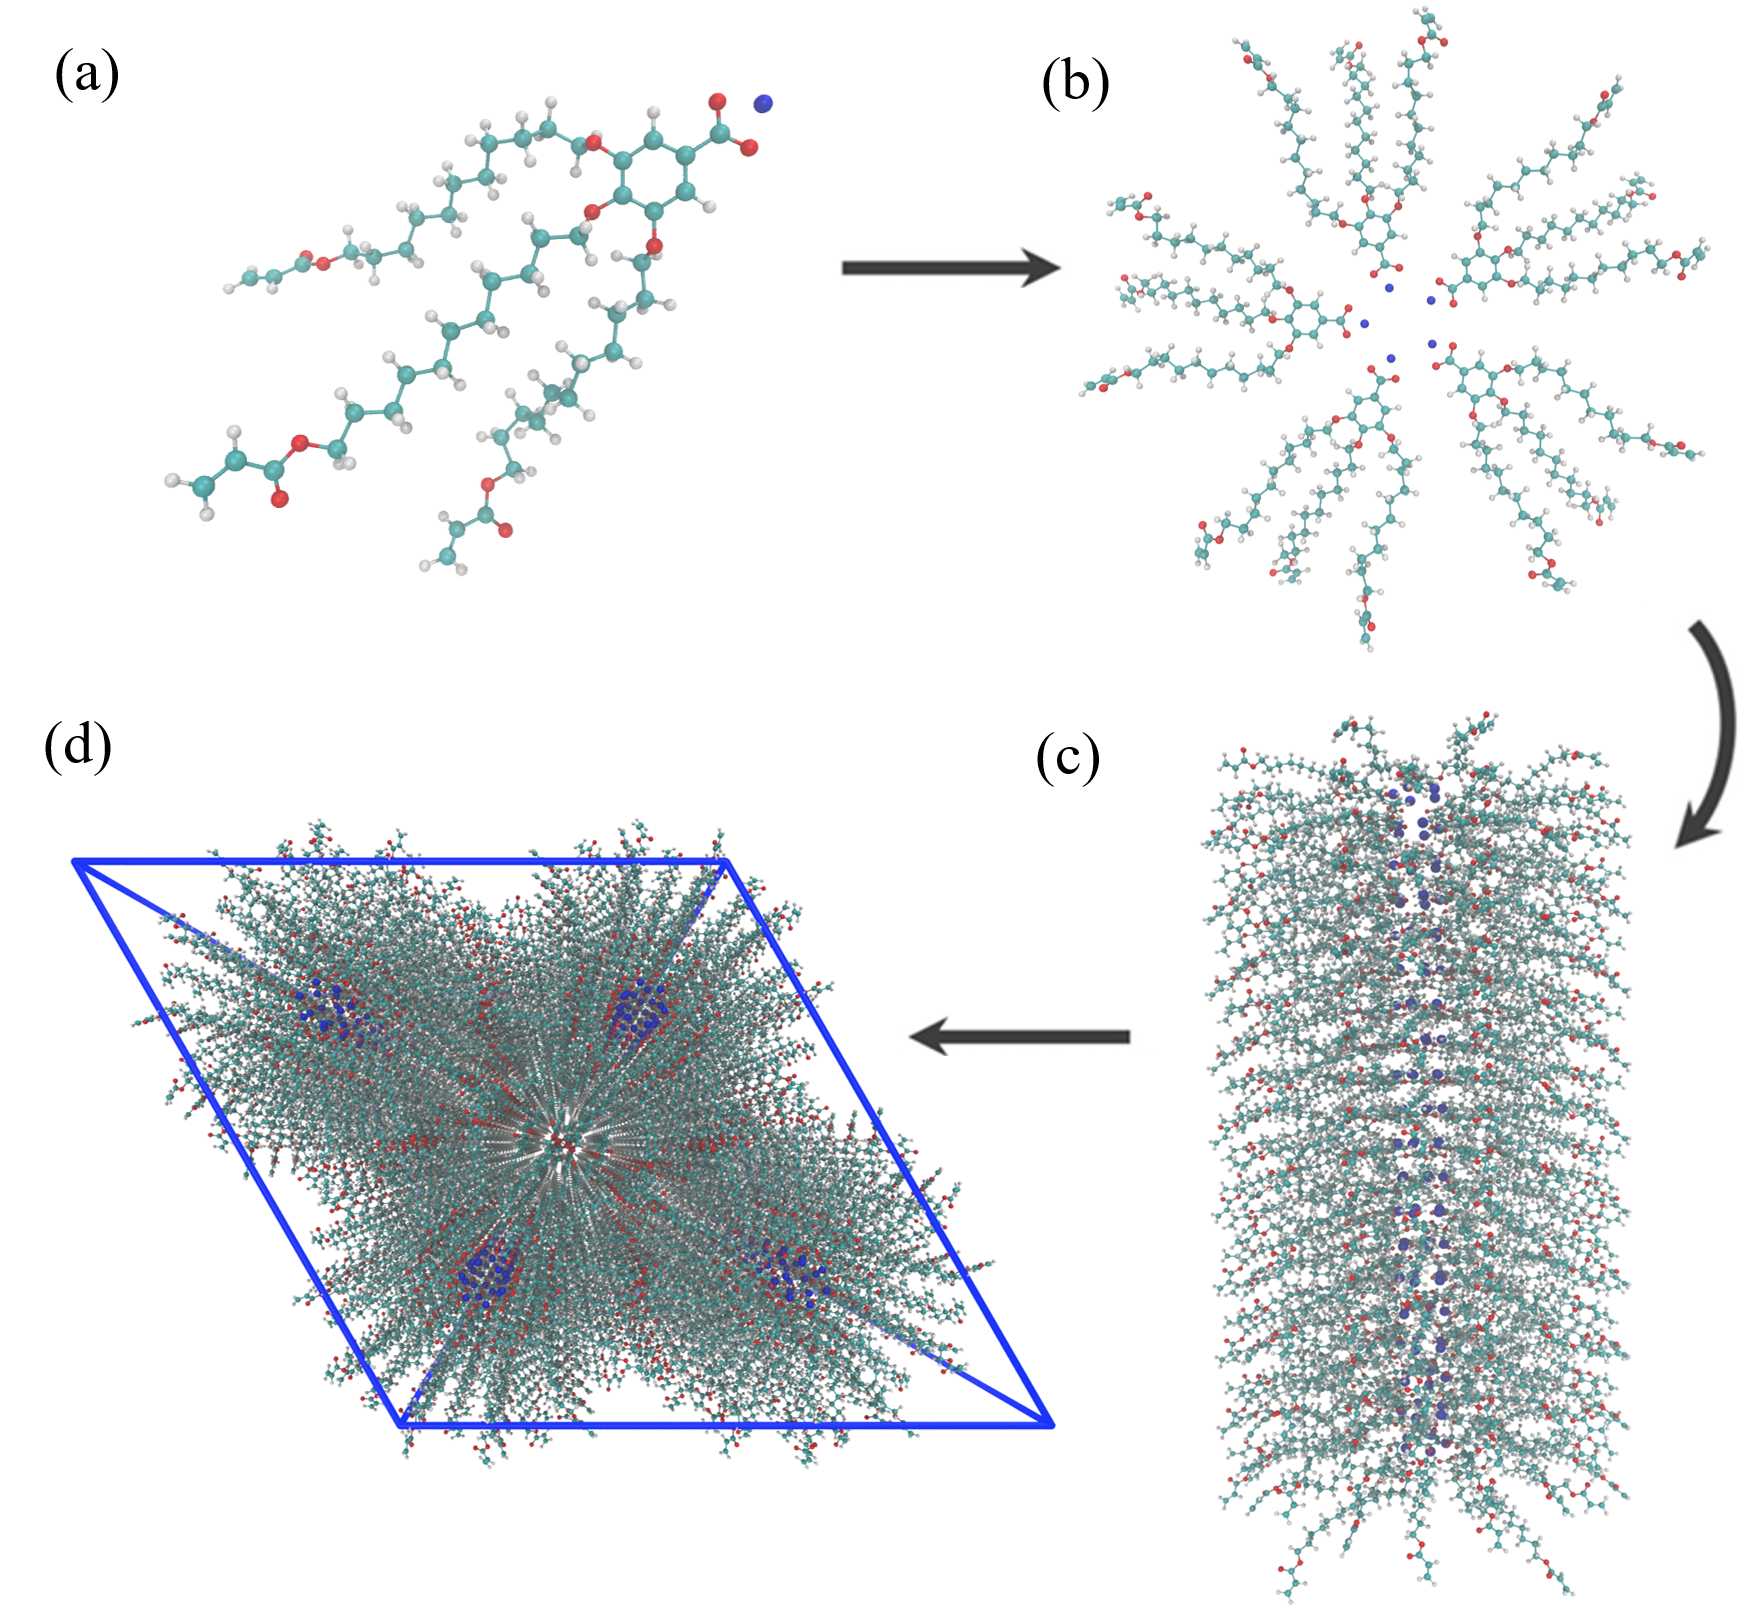
\includegraphics[width=0.75\linewidth]{build.PNG} %BJC: put an xyz axis with the unit cell
	\caption{(a) A single monomer was parameterized and annealed to produce a low energy
		configuration. (b) Monomers are rotated and assembled into layers with 
		hydrophlic centers. (c) Twenty layers are stacked on top of each other to create
		a pore. (d) Pores are duplicated and placed into a monoclinic unit cell}\label{fig:python}
  \end{figure}
  
  A typical simulation volume contains four pores in a monoclinic unit cell,
  the smallest unit cell that maintains hexagonal symmetry when extended 
  periodically.
  \begin{itemize}
    \item Each pore is made of twenty stacked monomer layers with periodic 
    continuity in the z direction, avoiding any edge effects and creating an 
    infinite length pore ideal for studying transport.
%    \item Each layer is made of a set number of monomers per layer, a variable to
%    be explored further.
    \item A small number of layers is preferred in order to reduce computational
    cost and to allow us to look at longer timescales.
    \item Ultimately, we chose to build a system with 20 monomer layers in each pore
    in order to obtain sufficient resolution when simulating X-ray diffraction patterns.
    This point will be explained in more detail later.
    %MRS: you should give the reasons in the same place you describe the choice, but the supporting data would probably be better in supporting information
    %BJC: so refer to supporting info here? Then put plots of diffraction data with different sized system there. I did not explain the resolution point here because I haven't talked about simulated X-ray diffraction yet and it wouldn't make sense. And it doesn't make sense to talk about XRD this early in the methods but I need to justify the number of layers.
    %MRS2: I was referring to the data choice of 20 vs 10.  Yes, you can refer to it here, because the expectation is that peple will only look at it after reading the whole paper.
%    \item We chose initial guesses for the remaining structural parameters based on
%    experimental data and treated them as variables during model development.
  \end{itemize}
 
%  We chose an initial layer spacing based on experimental 2D WAXS data.
%  \begin{itemize}  
%    \item The pattern shows reflections corresponding to features spaced 3.7 \angstrom~apart.
%    \item It has been hypothesized that the features are a result of $\pi$-$\pi$
%    interactions between stacked aromatic rings \cite{feng_scalable_2014}. 
%    \item Our simulations tend to equilibrate to a wider interlayer spacing of
%    $\approx$ 4.1 \angstrom~, which inspired separate systems starting with layer 
%    spacings greater than 4 \angstrom~.
%  \end{itemize}

  %%%%%%%%%%%% Monomer Placement %%%%%%%%%%%%%%
  
  When constructing an initial configuration, there are a number of variables
  which require careful consideration while placing monomers. The equilibrium
  configuration is sensitive to some while insensitive to others.
  \begin{itemize}
	\item The starting pore radius, defined as the distance of a chosen 
        head group carbon from the pore's central axis, does not influence the
        equilibrium structure when a reasonable value is chosen (See Supplemental)
        \item The pore radius is chosen to be 0.6 nm in our initial configurations 
        because the pore size is estimated to be $\approx$ 1.2 nm % Add reference
	\item The initial distance between pores also has little effect on the 
        the equilibrated structure. However, one should not start them too close or there 
        will likely be unintended high energy repulsions during early equilibration
	\item We chose an initial pore spacing of 4.5 nm, $\approx$ 10 \% larger than 
        the experimental value of 4.12 nm.
        \item The distance between layers and the rotation of the layers with respect
        to adjacent layers, and the number of monomers per layer do influence the 
        equilibrium structure and require further justification for their choices. 
        \item We rely on experimental data to inform our choices
  \end{itemize}

  We chose the layer spacing for the initial configuration based on R-$\pi$ 
  and then allowed system to readjust during equilibration.
  \begin{itemize}  
    \item Each monomer was rotated so the plane of the aromatic head groups would
    be coplanar with the xy plane.
    \item We explore two different initial layer spacings
    \item The first is exactly equal to R-$\pi$ with layers placed so aromatic
    rings are stacked 3.7 \angstrom~ apart in the z-direction.
    \item A second system is explored with an initial layer spacing of 5 \angstrom
%MRS3: at least state in the main body what went wrong with it in a sentence or so, with details in supplemental. 
   \item A third system with an initial layer spacing of 10 \angstrom was briefly
    explored
   \item When layers are spaced out sufficiently, they tend to collapse on each other 
   while simultaneously slipping in between layers of other pores which lead to an
   artificially thick membrane with pores spaced closely together.
   \item The intereseted reader can learn more about it in the Supplemental Information.
% BJC: Move all this lower down to be with the rest of the equilibrium calculations
%    \item To quantify the degree of layering in our system, we calculated
%    a spatial correlation function, $g(z)$, measured along the z-axis 
%    (perpendicular to the membrane plane)
%    \item To calculate $g(z)$, we binned the z component distances between 
%    the center of mass of each benzene ring and all others of the same pore 
%    over 50 ns of equilibrated trajectory and then normalized by the average
%    number density.
%    \item We compare the degree of layering between systems based on the
%    amplitude of the first peak in $g(z)$. We halve the difference between the
%    maximum of the first peak and the following minimum. We compare the difference
%    to the mean to get a percentage deviation from the average number density.
%    \item To extract the average distance between layers we applied a discrete 
%    fourier transform to $g(z)$ and extracted the highest intensity frequency 
  \end{itemize}

% BJC: removing this since I say earlier that the system is insensitive to this choice
% Detail will be provided in the supplement
% discussion of measuring equilibrium pore spacing is moved down to calculations part of methods
%  We placed pores at a chosen initial spacing based on R-pores, then allowed
%  the system to settle into its preferred spacing. 
%  \begin{itemize}
    %MRS: somewhere, should explain there's a large dependence of (meta)stable structures based on this initial distance.  It's sort of important to put somewhere.
    %BJC: Sure, but different choices of pore spacing were based on number of monomers per layer. More monomers per layer means a larger initial pore spacing.
%    \item The model's pore centers are spaced 4.5 nm apart initially, $\approx$ 10 \% larger
%    than the experimental value of 4.12 nm in order to reduce unintended repulsions 
%    resulting from a tightly packed initial configuration.
%    \item To calculate the equilibrated pore spacing, we measured the distance between pore
%    centers.
%    \item Pore centers were located by averaging the coordinates of sodium ions in their 
%    respective pores.
%    \item Statistics were generated using the bootstrapping technique (See Supplemental Information)
    	% Supplemental vvvv
%	\begin{itemize}
        %MRS2: make clear sampling what?
%        \item We are interested in 5 pore-to-pore distances which should all be equal in
%        a perfect hexagonal array, however only 4 distances are independent % can visualize this in supplemental material. Will make a lot of things more clear below.
%	\item Each pore spacing has its own trajectory of spacing vs. time. Using data collected after
%	the system is equilibrated, we calculate how long it takes for the data in each of the 5
%	trajetories to become uncorrelated using pymbar.timeseries.integratedAutocorrelationTime() % reference
%	\item We break the full trajectories down into sub-trajectories based on the
%	maximum autocorrelation time of those found in the previous step. 
%    	\item For each bootstrap trial, we recreate an equilibrium trajectory by randomly 
%    	sampling pore spacings from the sub-trajectories 
%    	\item We get an average value for each pore spacing by finding the mean of the bootstrapped data
%	\item We calculate the overall average as the mean of all bootstrapped pore spacings
%	\item The uncertainty for each pore spacing is calculated as $\dfrac{<x> - x}{4}$ where $<x>$ is the
%	average spacing from the bootstrap trial and $x$ is the average value of one of the pore spacings.
%	\item We report the mean of these uncertainties
        % MRS: need to deal with the fact only 4 are independent in the bootstrapping?  How did we do that?
	% BJC: Updated
        % Supplemental ^^^^
%	\end{itemize}
%  \end{itemize}
  
% BJC: This can be covered more in the Supplmental ... it might not even be necessary. I won't
% report any "pore sizes" except in the supplemental where I will show that the initial choice
% of pore radius has little effect on pore size

%  We used experimental Transmission electron microscopy (TEM) and size exclusion rejection
%  data \cite{feng_scalable_2014,feng_thin_2016,zhou_supported_2005} to inform our definition
%  of pore radius in the initial configuration.
%  \begin{itemize}
%    \item Experimental evidence suggests uniform pores with radii of 0.6 nm 
%    \item Comparing a geometric measurement of pore size derived from an atomistic model,
%    to a less precise, experimentally derived pore size estimate, will give ambiguous results.
%    \item What is meant by pore radius will not be clear until we establish a clear picture
%    of the nanoscopic pore environment.
%    \item When constructing pores, we chose the carboxylate carbon from the monomer
%    head group as a reference atom, and placed it a distance r from the pore center,
%    where r is the pore radius (~\ref{fig:pore_radius_illustration}). % BJC: Figure in Supplemental Information?
%    \item We will not make direct comparisons of pore radius between our model 
%    and experiment to avoid the ambiguity, however, we do define a pore radius  
%    for our own purposes.
    %\item To measure the pore radius in our model we calculate the distance between 
    %the center of mass of each aromatic ring and the center of mass of all aromatic rings
    %in their respective pores.
%  \end{itemize}

%MRS2: is the pore radius of the initial configuration really relevant? Does it need to be defined?  Seems like what radius means in the final equilibrated one is more important.
%BJC: This can go in supplemental
%  \begin{figure}
% 	\centering
% 	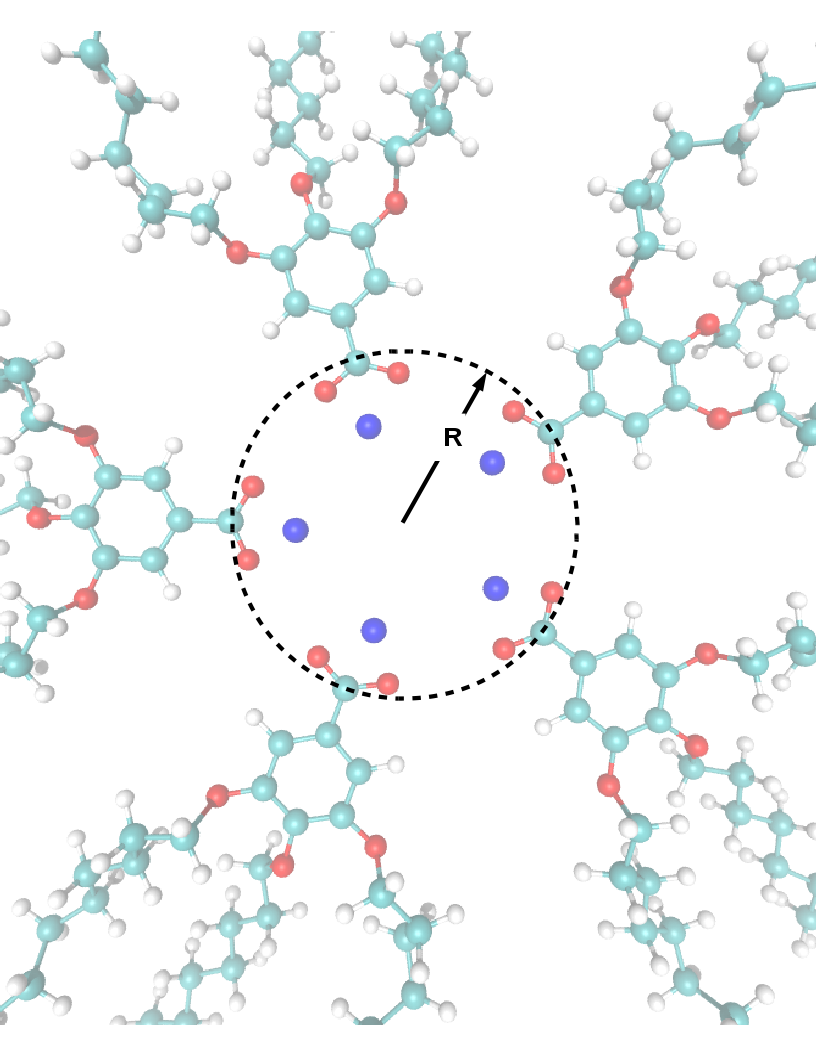
\includegraphics[width=\textwidth]{pore_radius_illustration.png}
%	\caption{The pore radius of the initial configuration is defined using the 
%        carboxylate carbon as a reference}~\label{fig:pore_radius_illustration}
%  \end{figure}
  
  The relative interlayer orientation was chosen based on clues from 
  diffraction data as well as the various known stacking modes of benzene 
  and substituted benzene rings: sandwiched, parallel-displaced and T-shaped
  ~\cite{sinnokrot_estimates_2002} (\Cref{fig:sandwiched,fig:pd,fig:tshaped}).
  \begin{itemize}
    \item The T-shaped configuration was ruled out based on the inconsistency of
    its $\approx$ 5 \angstrom~equilibrium stacking distance ~\cite{sinnokrot_estimates_2002}.
    \item The system's preference towards the sandwiched vs. parallel displaced 
    stacking modes will be explored.
    \item Both have reported stacking distances near the R-$\pi$ value of 3.7 \angstrom % Reference
    \item Headgroups in our sandwiched initial configuration are stacked directly
    on top of each other while stacked headgroups in the parallel displaced 
    initial configuration are offset by $180/nmon$ degrees where $nmon$ equals
    the number of monomers per layer.
    %BJC: I think the following commentary belongs elsewhere, maybe even in the discussion
    %MRS: hard to say. It's certainly a big switch from things that are relatively straightforward to things that require 
    % a fair amount of information, so I think it belongs in it's own section -- so far, you're just laying out the approach.  This is what we fix, this is what we leave as a variable.  The analysis probably belongs later.
    %BJC: Yeah, I will leave the rest for discussion
%     \item Visualization of each configuration (\Cref{fig:sandwichedlayers,fig:offsetlayers})
%     suggests entropic differences based on the way the tails are able to pack.
%     \item In the sandwiched configuration, all tails start out directly on top
%     of each other which may prevent closely stacked benzene rings.
%     \item In the offset configuration, the tails are placed in between each other 
%     which may allow layers to come together in a compact way.
%     \item This difference may explain, in part, which stacking mode is more favorable.
  \end{itemize}

  As outlined in \ref{point:monomernum} the number of monomers in each layer is unknown
  so we tested configurations constructed with a varied number of monomers per layer.
  \begin{itemize}
	\item Systems were built in the offset and parallel displaced configurations
        with 4, 5, 6, 7 and 8 monomers per layer
  \end{itemize}

  %%%%%%%%%%%% Equilibration %%%%%%%%%%%%%%

  We developed equilibration schemes to create dry and wet configurations. Both schemes 
  start with an initial configuration generated according to the previous guidelines.
  \begin{itemize}
      \item Dry equilibration scheme:
      \begin{itemize}
        %MRS2: what initial force constant, and does it matter (that can be in supplemental) 
	%BJC: I've never explored whether there is any dependence on initial force constant. It probably doesn't matter unless it starts really low
        %MRS3: then just state what you did, so it could be repeated. 
          \item Restraints with a force constant of 1e6 KJ mol$^-1$ nm$^-2$, fix monomer 
	  head groups in the sandwiched or parallel-displaced configurations while 
          allowing monomer tails to settle.
          \item Doing so also mitigates system dependence on initial monomer configuration.
          \item The restrained portion of the equilibration scheme is run in the NVT ensemble.
          \item Every 50 ps, we reduce the force constants by the square root of its
          previous value %, starting from 1e6 KJ mol$^-1$ nm$^-2$. <-- stated in first bullet
          \item Once the force constant is below 10 KJ mol$^-1$ nm$^-2$, the restraints are
          released linearly until there is no more restraining potential.
          \item The resulting unrestrained structure is allowed to equilibrate for 5 ns 
	  in the NPT ensemble with pressure controlled by the berendsen barostat.
	  \item Long, NPT equilibration simulations are run for at least 400 ns using the 
          Parrinello-Rahman barostat with a time consant of 10 ps.
          %MRS5: did you ever look at isotropic vs. semiisotropic? If using isotropic, you should look at the pressure tensor - if the Z is very different than the X and Y and has opposite sign, the membrane could be under strain in some way despite being at 1 atm.
      \end{itemize}
      \item Wet equilibration scheme: 
      \begin{itemize}
	  % BJC: the following three bullet points ended up not being the case since I used significantly less water
          %\item We obtained an estimate of equilibrium pore water content by solvating
          % an initial configuration with water baths above and below the membrane. 
	  %\item We ran the solvated system according to Scheme A but with a 1000 ns equilibration
          %\item Using that number we added water to the pores of an initial 
	  %configuration and equilibrated according to scheme B. 
	  \item In order to create a wet system, we solvated an initial configuration with water using gmx solvate
          \item All water molecules placed outside the pore region are removed 
	  \item Waters inside the pore region are randomly removed until the desired concentration
	  of water in the pores is reached. 
	  \item The remainder of the equilibration is the same as the dry system
      \end{itemize}
      \item In all cases, the v-rescale thermostat was used with tau-t = 0.1 % BJC: supplemental
  \end{itemize}

%  An equilibration scheme with position restraints placed on aromatic rings
  %MRS: 
  %prevents 
%  during early equilibration steps is required to prevent high energy repulsions .
  %MRS: should be clearer what you mean by ``unrealistic jumps''.  Hard to visualize.
  %BJC: 'high energy repulsions' ?
%  \begin{itemize}
%    \item Restraints fix monomer head groups in the sandwiched or parallel-displaced
%    configurations while allowing monomer tails to settle.
%    \item Doing so also mitigates system dependence on initial monomer configuration.
%    \item The restrained portion of the equilibration scheme is run in the NVT ensemble.
%    \item Every 50 ps, we reduce the force constants by the square root of its 
%    previous value, starting from 1e6 KJ mol\textsuperscript{-1} nm\textsuperscript{-2}.
%    \item Once the force constant is below 10 KJ mol\textsuperscript{-1} 
%    nm\textsuperscript{-2}, the restraints are slowly released until there is no more 
%    restraining potential.  
%    \item The resulting unrestrained structure is allowed to equilibrate further in the NPT
%    ensemble for 400 - 500 ns.
   %BJC: I will reference an equilibration script that can be released with the supplemental info
   %MRS: we should release as many scripts as is feasible, can be in a github repository.
   %BJC: Okay, once we submit, I will need to spend some time cleaning the scripts
   %MRS: You've described two equilibration procedures (or two varieties of the same one?) - need to be crystal clear to the reader as to which is used where.
   %BJC: Yea I'm just saying that I do 50 ps restrained simulations in NVT ensemble and then once the restraints are gone I switch to NPT. I edited the language to try and make it clearer.
%  \end{itemize}
  
  %BJC: the following paragraph will be replaced with something that Joe writes
  %MRS: sounds good.
  
  % BJC: The following methodology is taken from the 2014 Feng et al. paper where
  % WAXS is reported. The data we are using comes from the 2016 paper which 
  % I assume used the same set up but I will need to verify this with Xunda
  % before this gets sent out. The SAXS is the same as shown in the 2016 paper
  % however I will likely reproduce it with matplotlib 
  
  %Experimental wide angle X-ray scattering measurements were performed using a 
  %Rigaku 007 HF+ instrument with a rotating anode Cu K$\alpha$ X-ray source
  %($\lambda$~= 1.542 \angstrom~) and a 2-D Saturn 994+ CCD detector. The 
  %calibrations of the resultant 2-D WAXS patterns were done by using a 
  %silicon powder standard (d-spacing of 3.1355 \angstrom~). 2-D SAXS scattering
  %patterns were integrated into 1-D plots of scattering intensity (I) versus
  %q, where q = 4$\pi$sin($\theta$)/$\lambda$ and the scattering angles is
  %2$\theta$. The data shown is reproduced from data collected elsewhere~\ref{feng_scalable_2014}.

%%%%%%%%%%%%% Crosslinking %%%%%%%%%%%%

  Using an equilibrated structure, a crosslinking procedure was performed
  in order to match synthetic procedures.
  \begin{itemize}
    \item The purpose of crosslinking is to maintain macroscopic alignment of
    the crystalline domains, ensuring aligned, hexagonally packed pores.
    \item For that reason, we are not concerned with replicating the kinetics
    of the reaction, but instead emphasize the consistency of the final structure
    with experimental structural data.
    \item The algorithm was developed based on the known reaction mechanism.
    \item Crosslinking of this system is a free radical polymerization (FRP)
    taking place between terminal vinyl groups present on each of the three
    monomer tails.
    \item FRPs require an initiator which bonds to the system, meaning new atoms
    were introduced into the system.
    \item For simplicity, the initiator was simulated as hydrogen and made present
    in the simulation by including them in all possible bonding positions as dummy atoms.
    \item The crosslinking procedure is carried out iteratively.
    \item During each iteration, bonding carbon atoms are chosen based on a distance cut-off.
    \item The topology is updated with new bonds and dummy hydrogen atoms are
    changed to appropriate hydrogen types.
    \item Head-to-tail addition was the only propagation mode considered due to
    its dominance in the real system.
    \item Direction of attack was not considered because the resultant mixture
    is racemic.
    %MRS5: if this is not that important to the results, some of these details could potentially be in the supporting information.
    %BJC: The following items belongs in results/discussion
    %MRS: probably. 
    %\item The resulting crosslinked structure has an even distribution of
    %crosslinks between monomer tails of the same monomer, monomers stacked on
    %top of each other and monomers in other pores, including across periodic
    %boundaries.
    %\item The pore spacing shrinks by $\approx$ 1 \angstrom~ and stays 
    %constant under a range of simulation conditions.
  \end{itemize}

%%%%%%%%%%%%% Equilibrium Calculations %%%%%%%%%%%%%%%

  Using equilibrated structures, we carry out various calculations to characterize the
  system. 
  \begin{itemize}
	\item We determine the point at which a system is equilibrated when the 
        distance between pores stops changing
  \end{itemize}

  To calculate the equilibrated pore spacing, we measured the distance between pore
  centers.
  \begin{itemize}
	\item Pore centers were located by averaging the coordinates of sodium ions in their
	respective pores.
	\item Statistics were generated using the bootstrapping technique (See Supplemental Information)
	% Supplemental vvvv
        \begin{itemize}
        	%MRS2: make clear sampling what?
	        \item We are interested in 5 pore-to-pore distances which should all be equal in
	        a perfect hexagonal array, however only 4 distances are independent % can visualize this in supplemental material. Will make a lot of things more clear below.
	        \item Each pore spacing has its own trajectory of spacing vs. time. Using data collected after
	        the system is equilibrated, we calculate how long it takes for the data in each of the 5
	        trajetories to become uncorrelated using pymbar.timeseries.integratedAutocorrelationTime() % reference
	        \item We break the full trajectories down into sub-trajectories based on the
	        maximum autocorrelation time of those found in the previous step.
	        \item For each bootstrap trial, we recreate an equilibrium trajectory by randomly
	        sampling pore spacings from the sub-trajectories
	        \item We get an average value for each pore spacing by finding the mean of the bootstrapped data
	        \item We calculate the overall average as the mean of all bootstrapped pore spacings
                  %MRS3: this sounds a little convoluted below.  Should just be the standard error in the boostrap estimates of the pore spacing?
                  %MRS3: this can be fixed in the draft not outline.
	        \item The uncertainty for each pore spacing is calculated as $\dfrac{<x> - x}{4}$ where $<x>$ is the
	        average spacing from the bootstrap trial and $x$ is the average value of one of the pore spacings.
	        \item We report the mean of these uncertainties
	        % MRS: need to deal with the fact only 4 are independent in the bootstrapping?  How did we do that?
	        % BJC: Updated
        \end{itemize}
        % Supplemental ^^^^^
  \end{itemize}

  To quantify the degree of layering and the equilibrium distance between layers
  in our system, we calculate a spatial correlation function, $g(z)$, measured
  along the z-axis (perpendicular to the membrane plane).
  \begin{itemize}
    \item To calculate $g(z)$, we binned the z component distances between
    the center of mass of each component and all others of the same pore
    over at least 50 ns of equilibrated trajectory and then normalized by the 
    average number density.
%    \item We compare the degree of layering between systems based on the
%    amplitude of the first peak in $g(z)$. We halve the difference between the
%    maximum of the first peak and the following minimum. We compare the difference
%    to the mean to get a percentage deviation from the average number density.
    \item To extract the average distance between layers we applied a discrete
    fourier transform to $g(z)$ and extracted the highest intensity frequency
  \end{itemize}

  % BJC: To be replaced by Joe's description
  Simulated X-ray diffraction patterns were generated based on atomic
  coordinates for a direct experimental comparison.
  \begin{itemize}
    \item All atomic coordinates were simulated as gaussian spheres of electron
    density corresponding to each atom's atomic number.
    \item A three dimensional fourier transform (FT) of the array of electron 
    density results in a three dimensional structure factor which represents
    the unit cell in reciprocal space.
   % \item We perform an angular average of the structure factor about the 
    z axis to generate a 2D cross section close to what one would see 
    experimentally.
    \item We matched experimental 2D WAXS patterns by adjusting the initial 
    spacing between layers and the orientation of the head groups with respect
    to adjacent layers.
  \end{itemize}
  
  % BJC: I think this figure belongs somewhere else
  \begin{figure}
	\centering
	\begin{subfigure}[b]{0.32\textwidth}
		\centering
		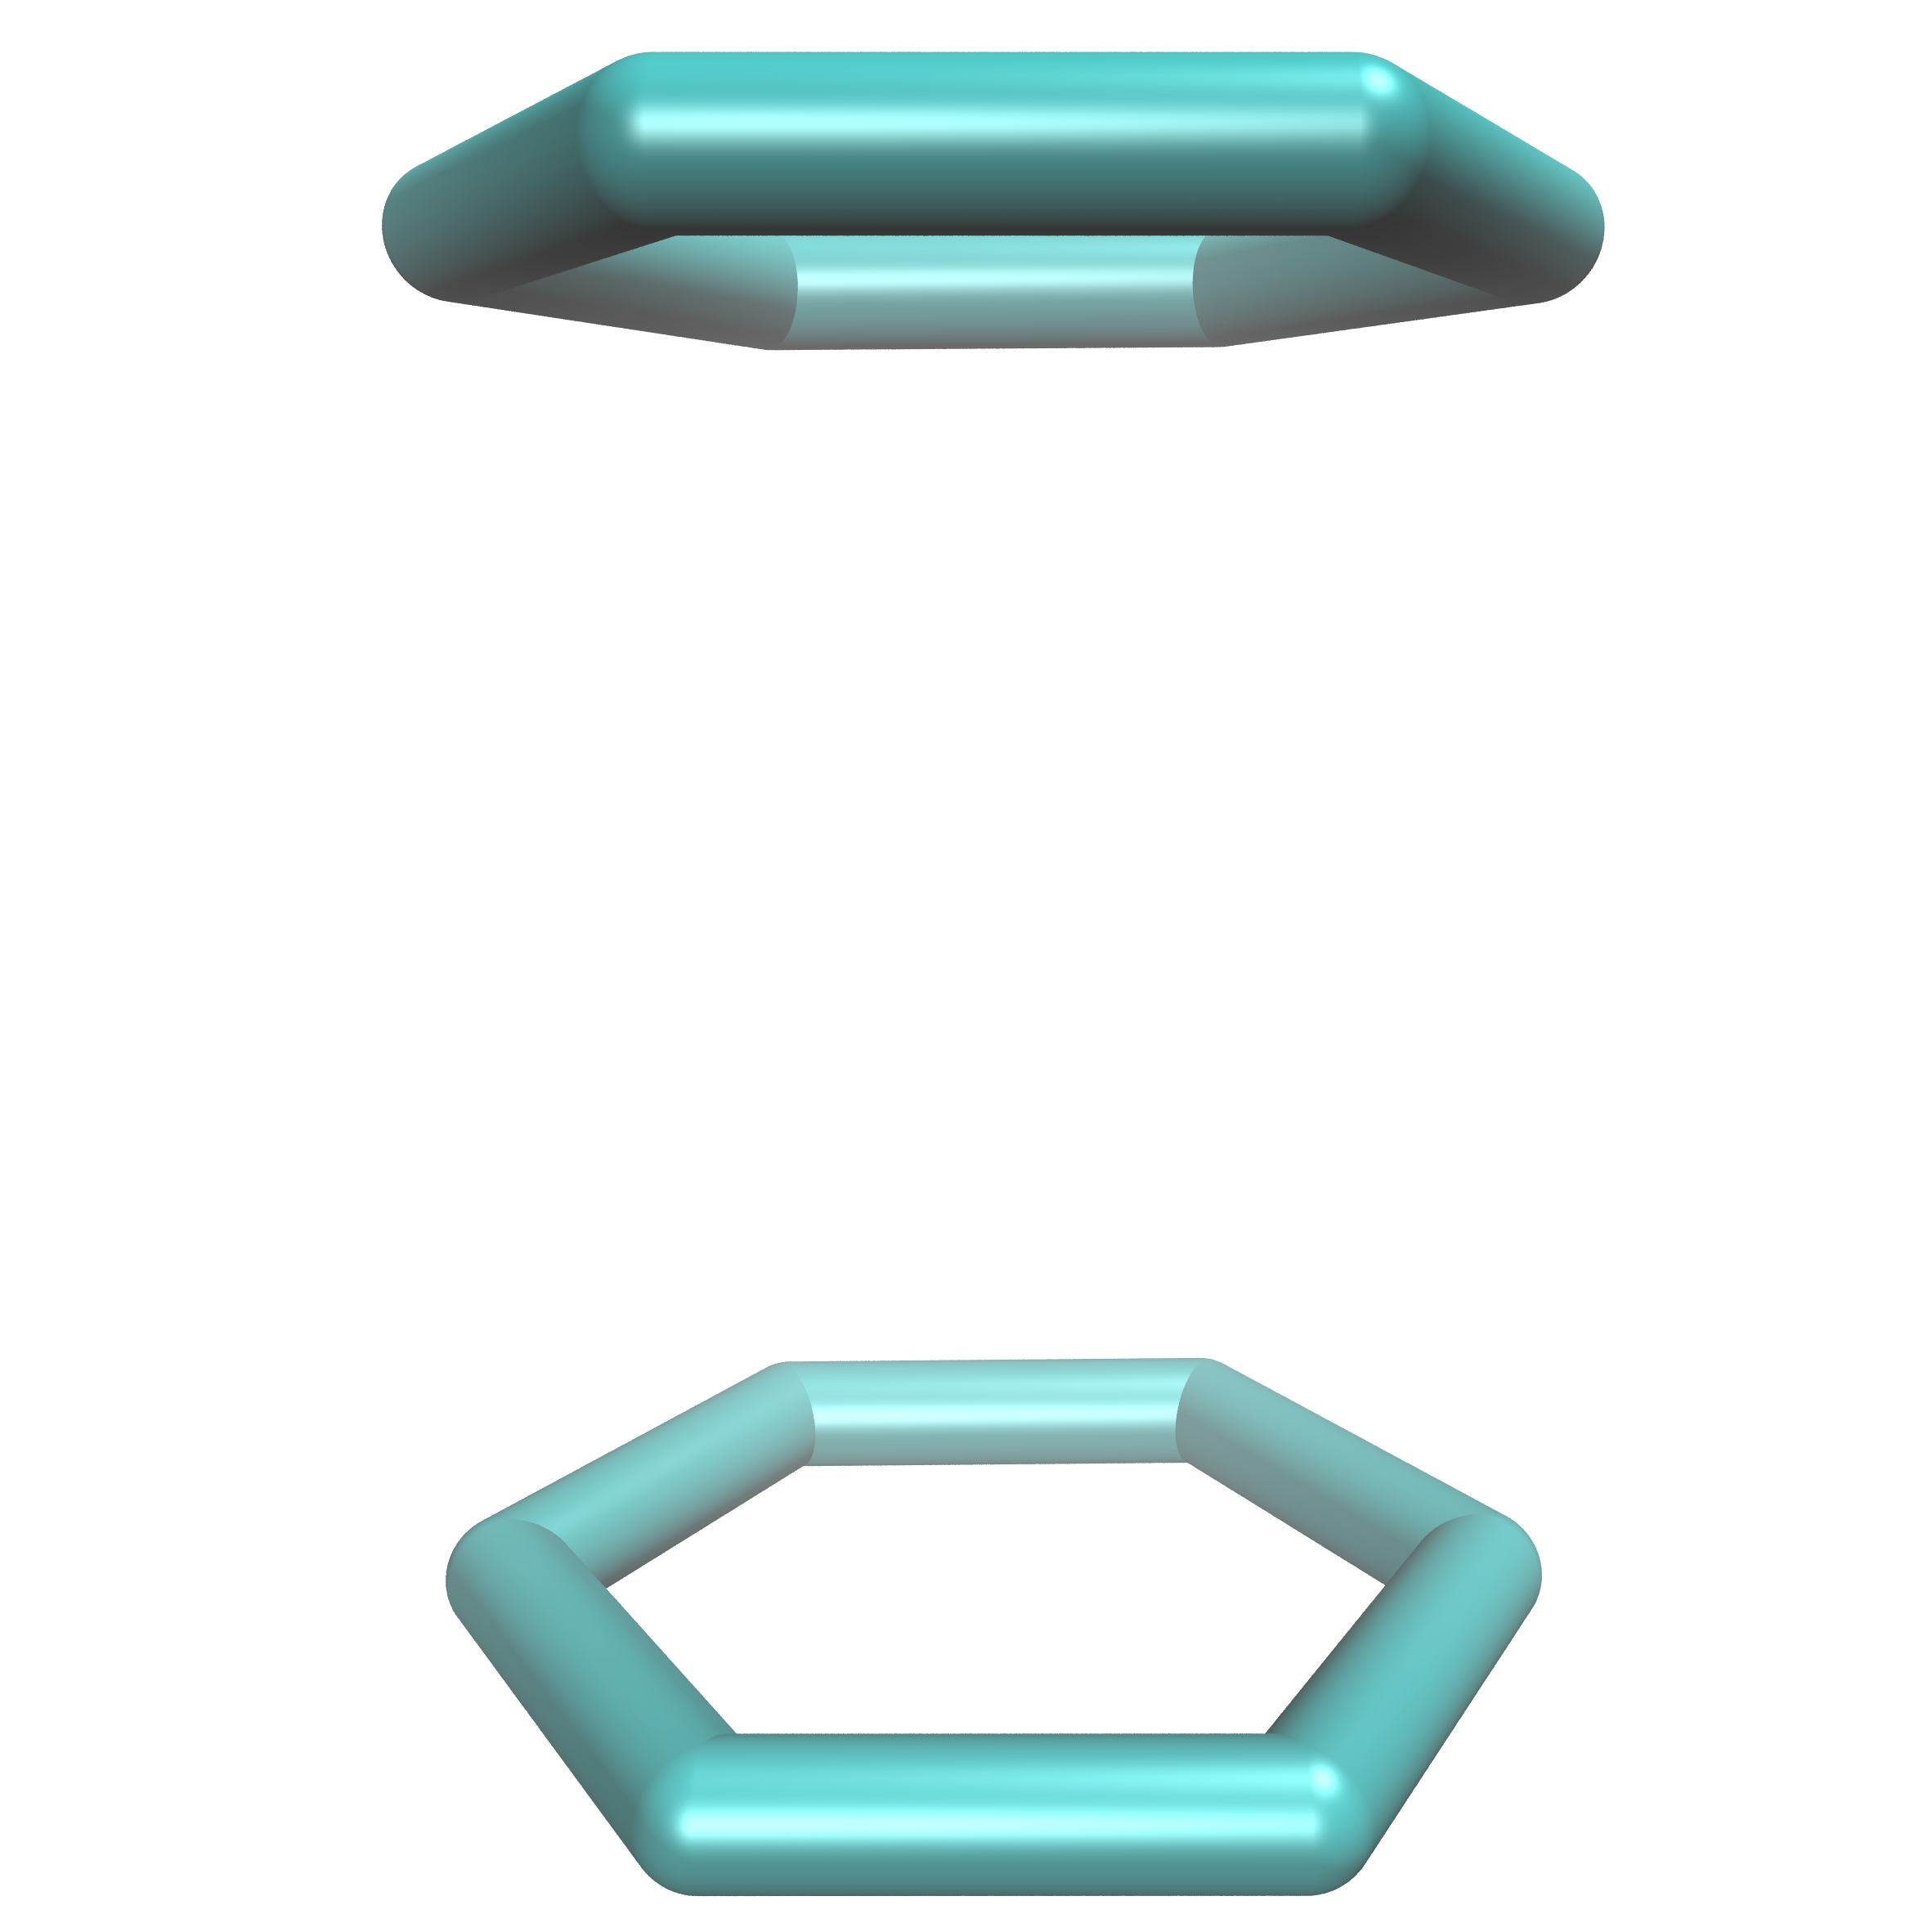
\includegraphics[width=\textwidth]{sandwiched.png}
		\caption{}\label{fig:sandwiched}
	\end{subfigure}
	\begin{subfigure}[b]{0.32\textwidth}
		\centering
		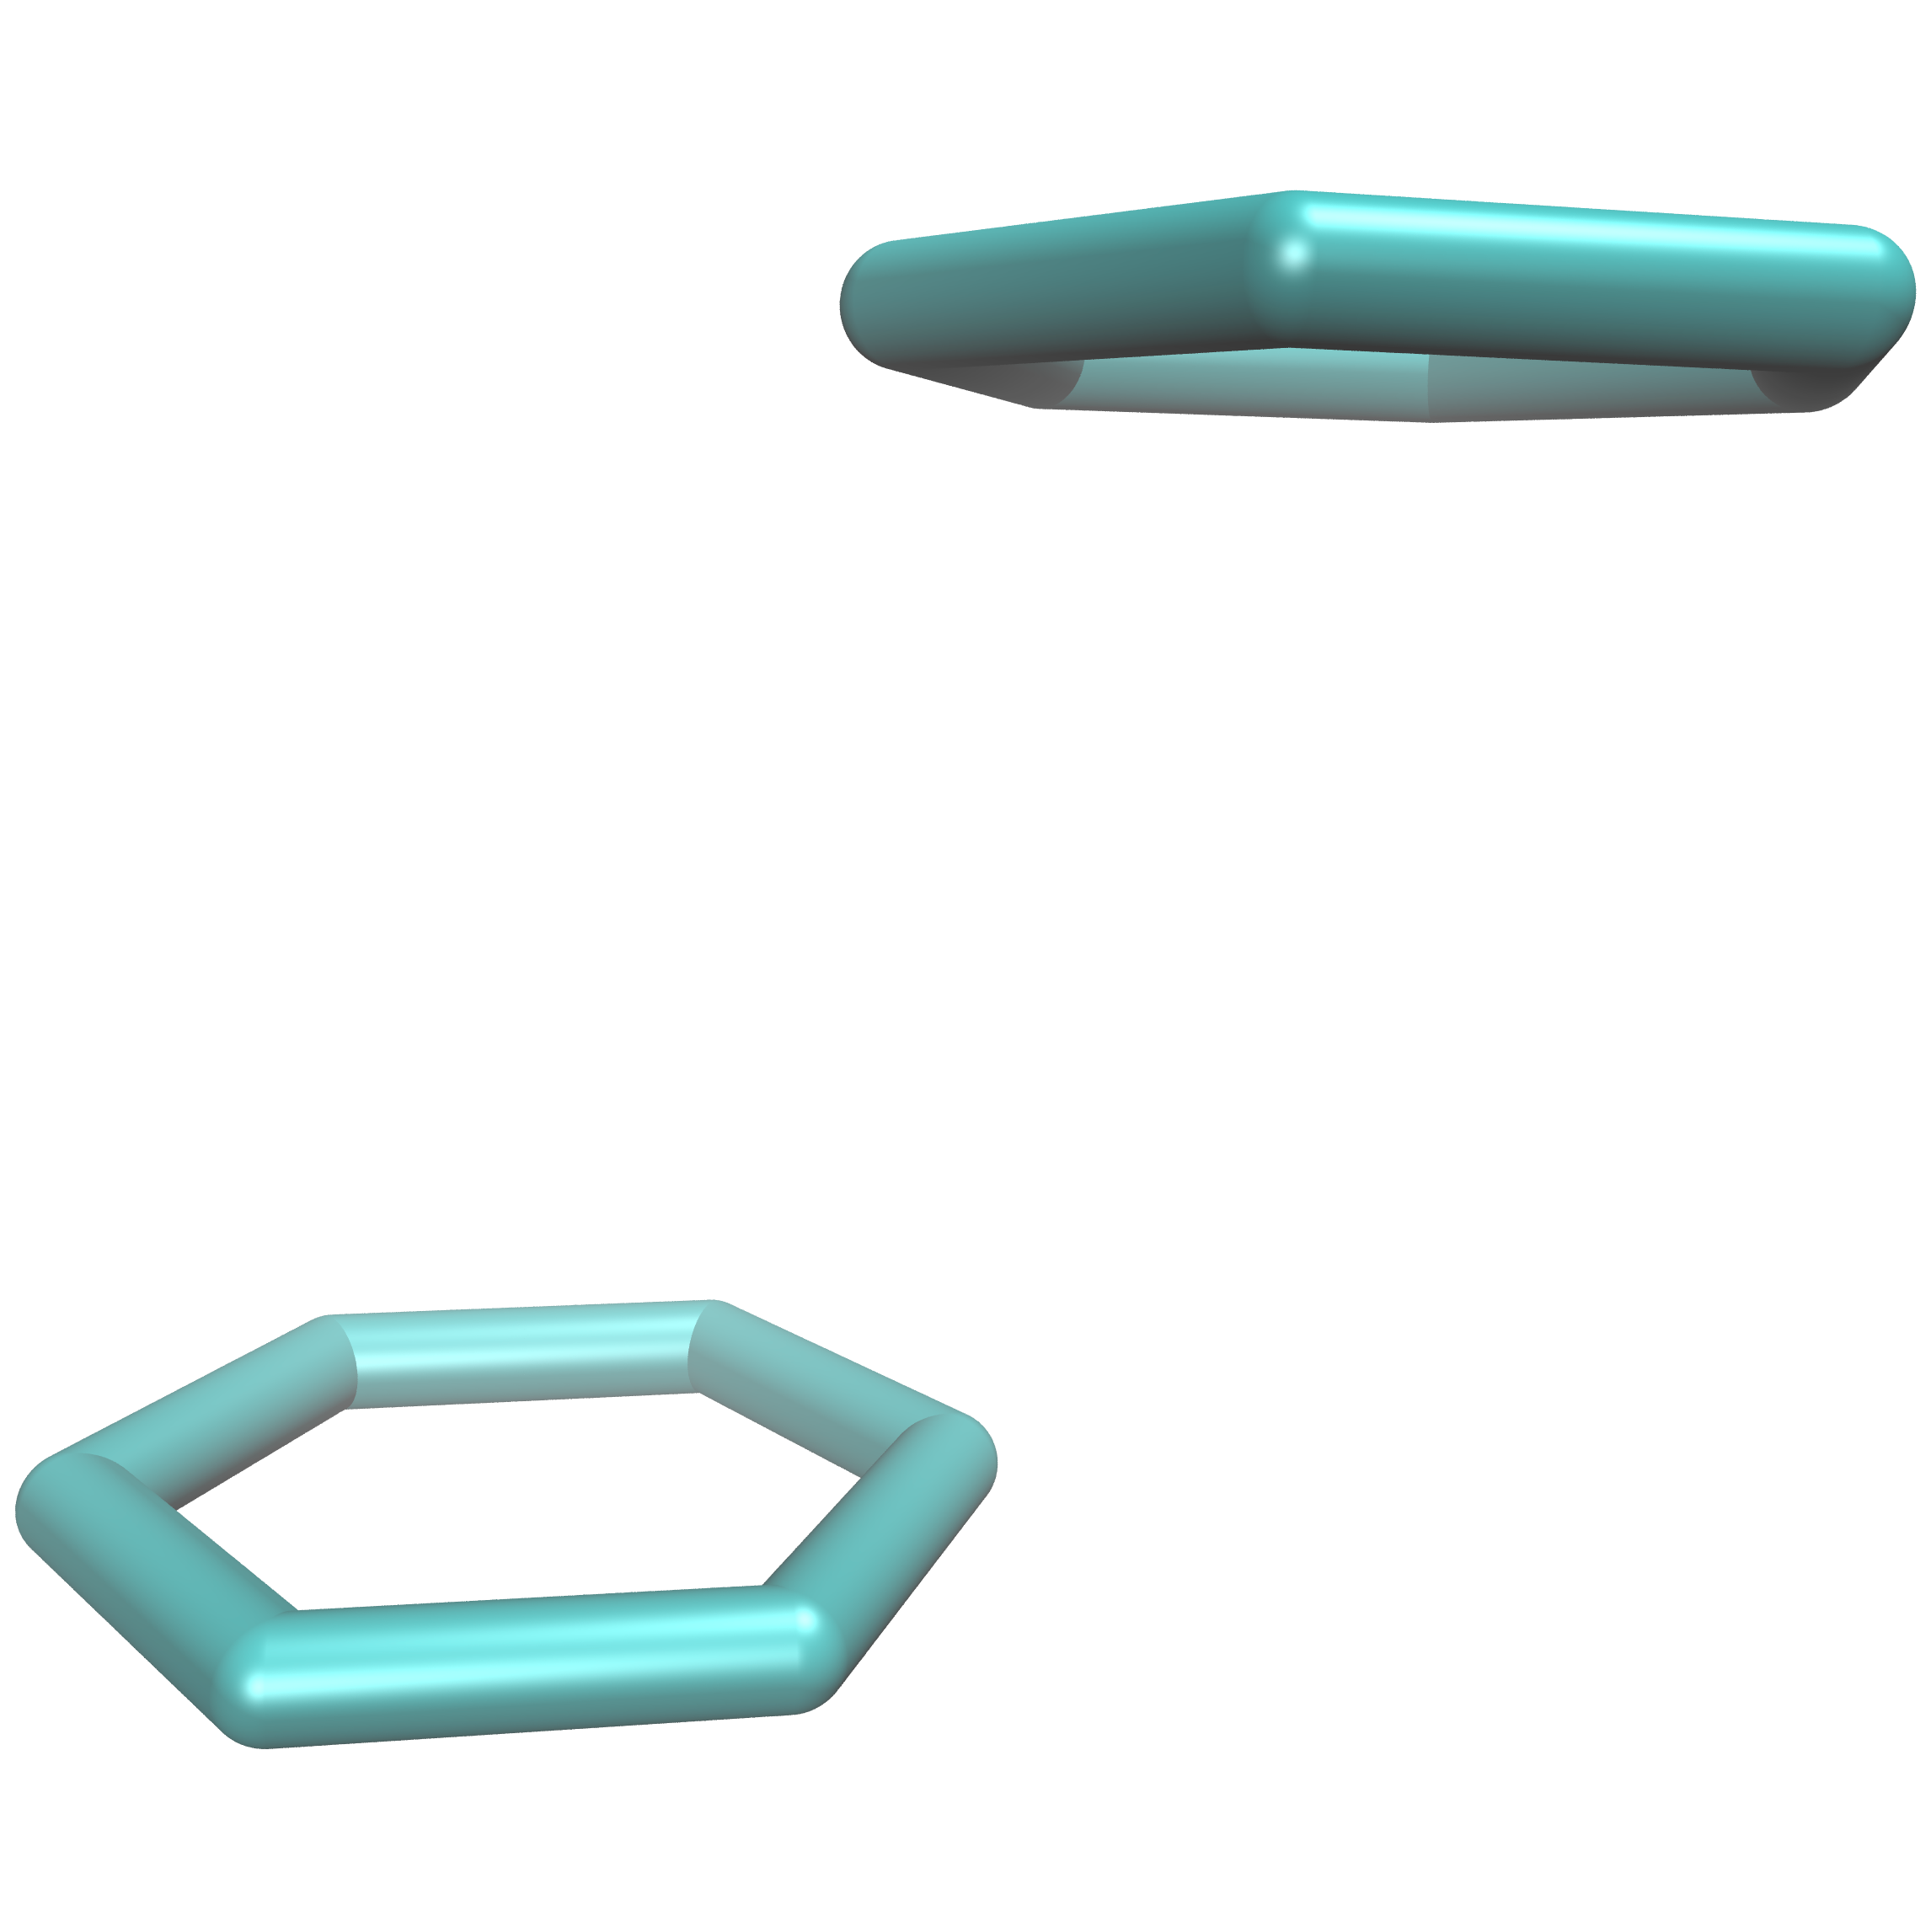
\includegraphics[width=\textwidth]{PD.png}
		\caption{}\label{fig:pd}
	\end{subfigure}
	\begin{subfigure}[b]{0.32\textwidth}
		\centering
		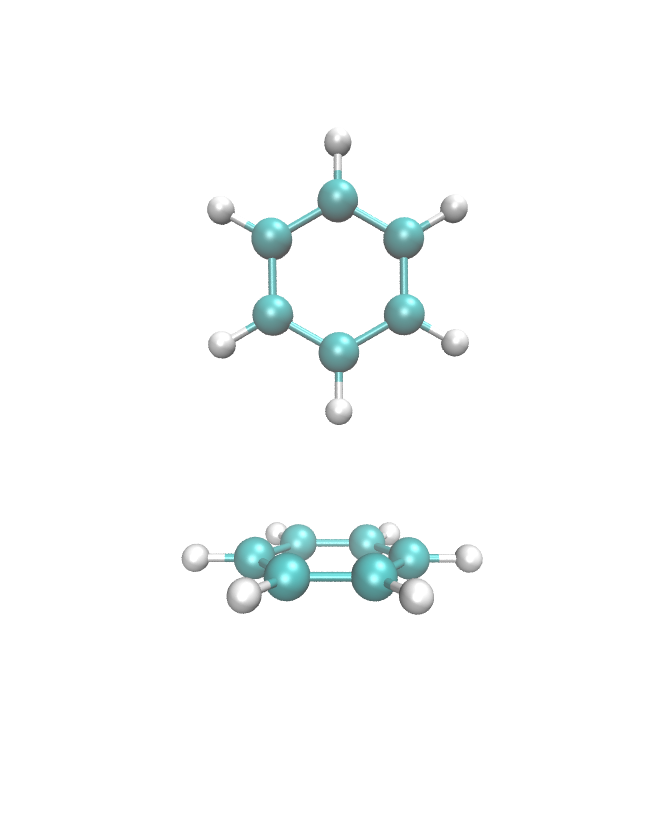
\includegraphics[width=\textwidth]{Tshaped.png}
		\caption{}\label{fig:tshaped}
	\end{subfigure}
	\vskip\baselineskip
	\begin{subfigure}[b]{0.475\textwidth}
		\centering
		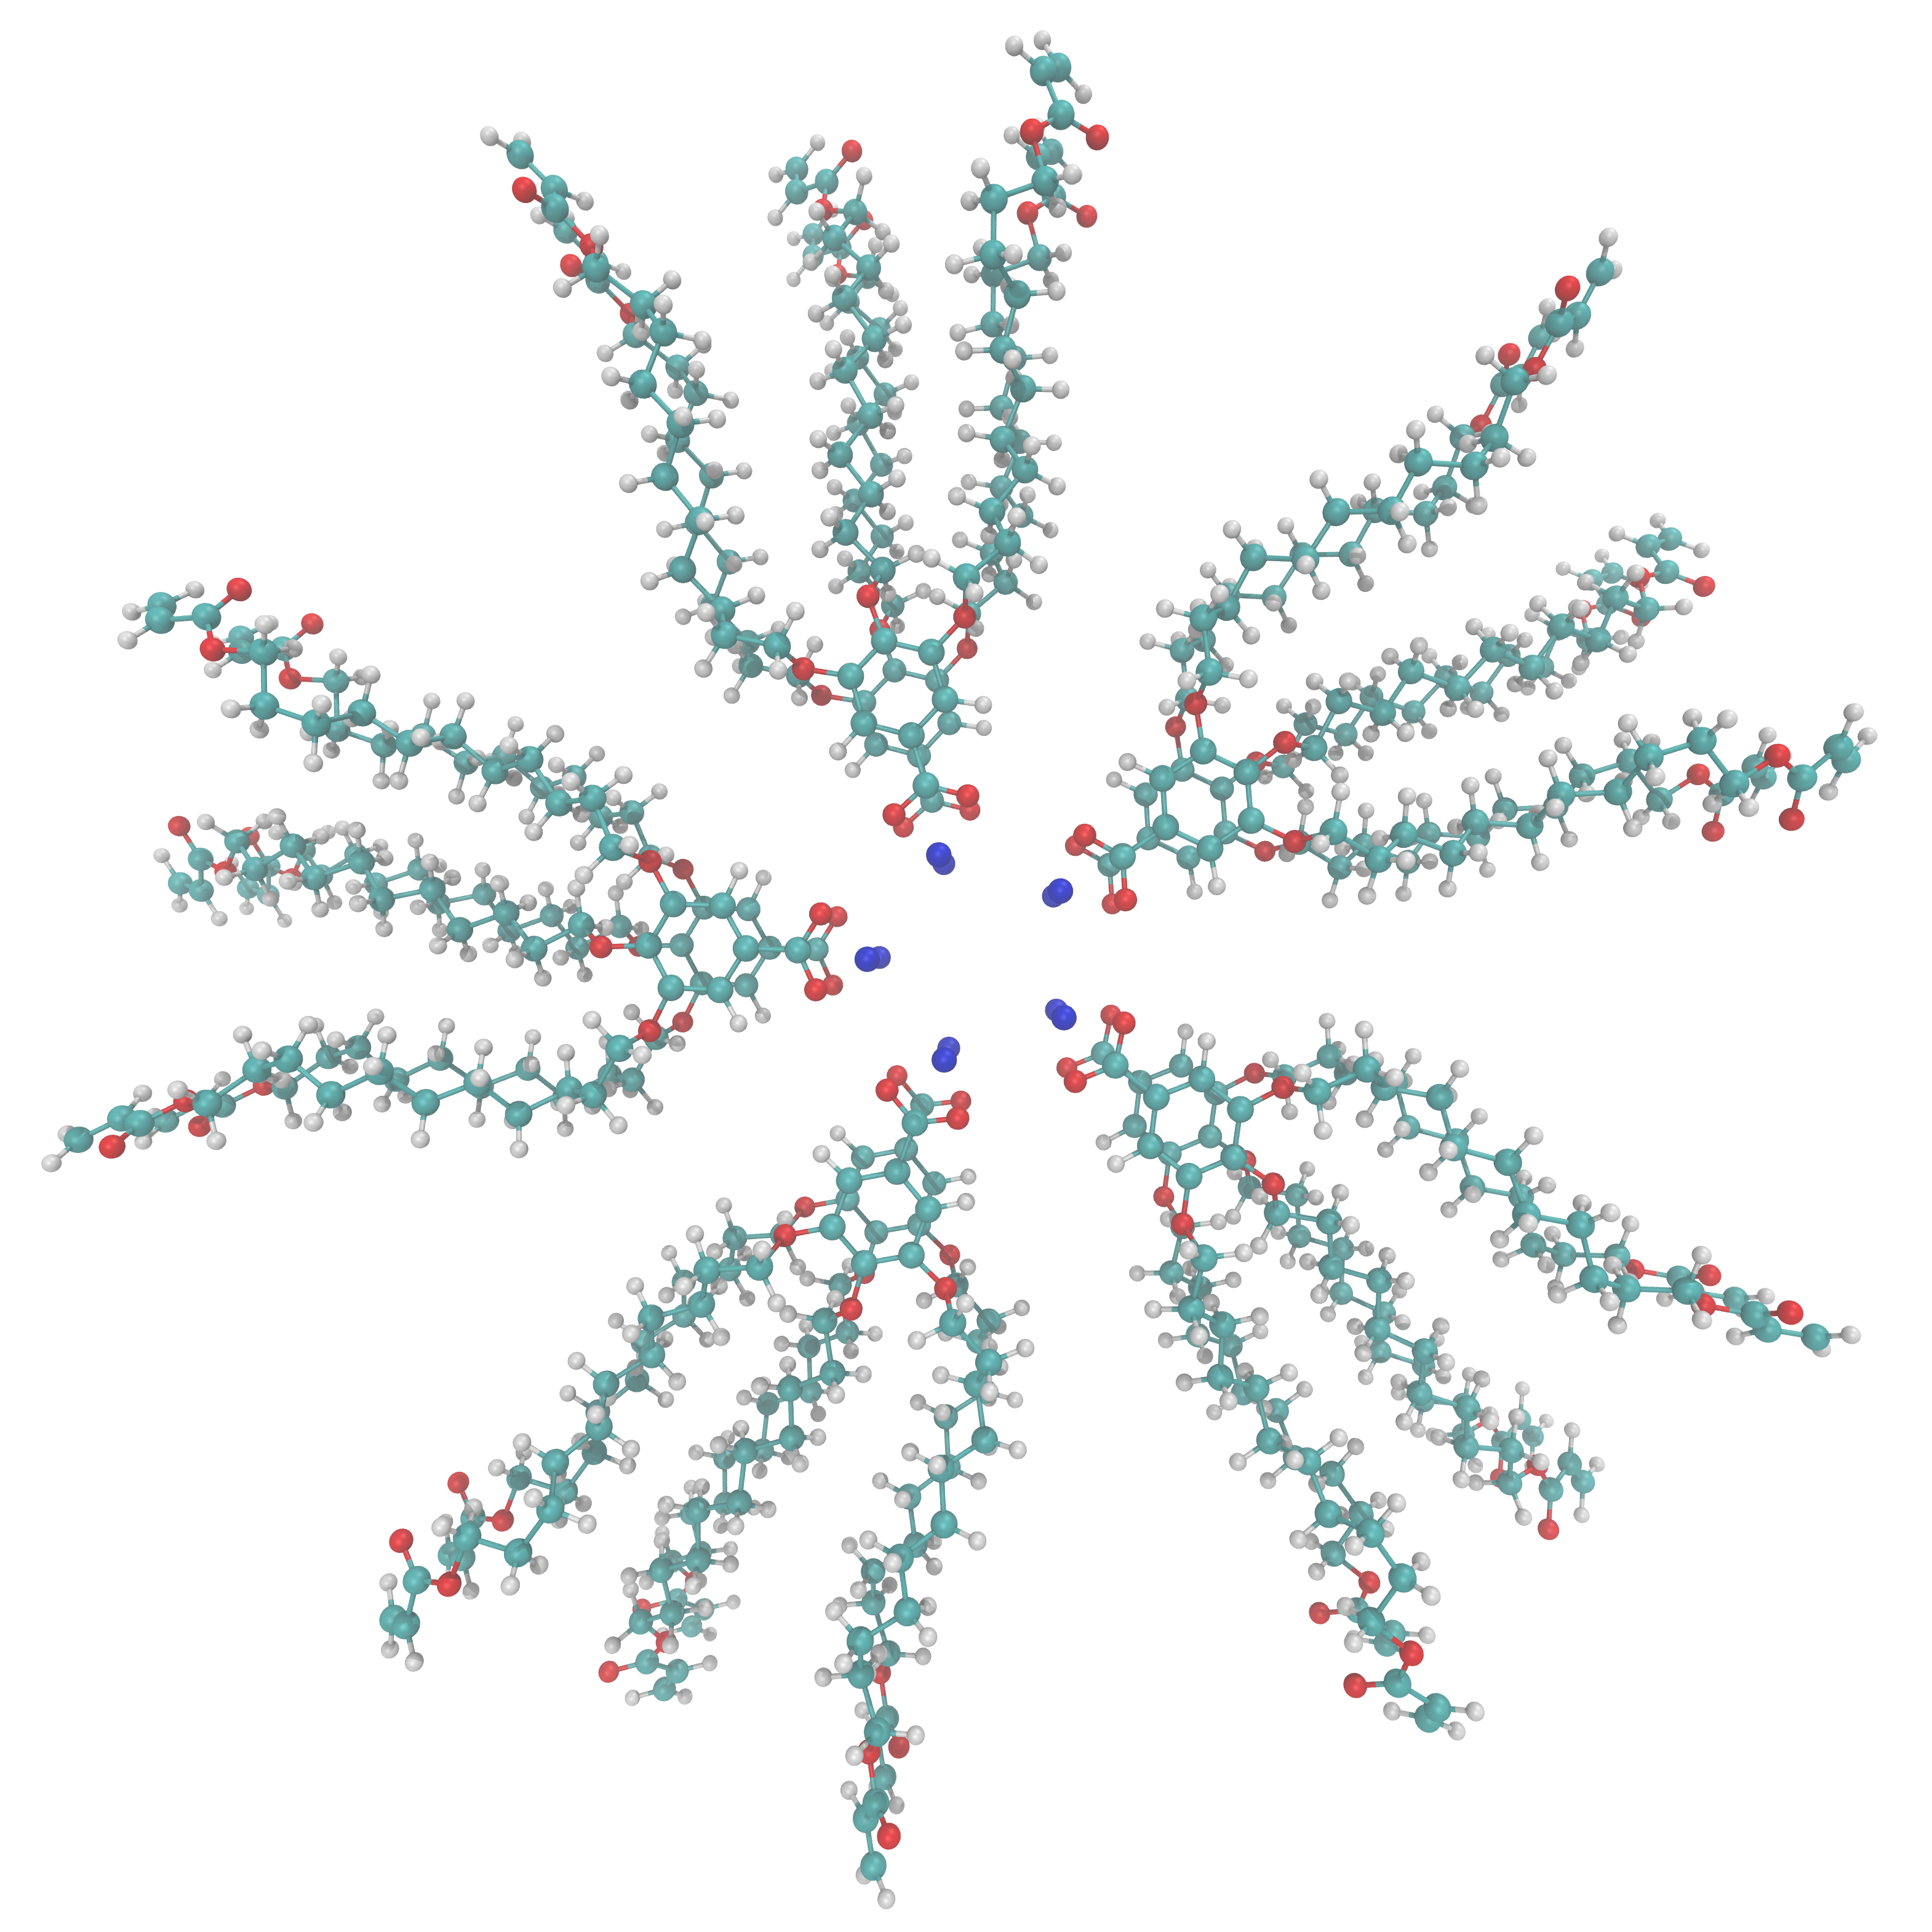
\includegraphics[width=\textwidth]{sandwichedlayers.png}
		\caption{}\label{fig:sandwichedlayers}
	\end{subfigure}
	\begin{subfigure}[b]{0.475\textwidth}
		\centering
		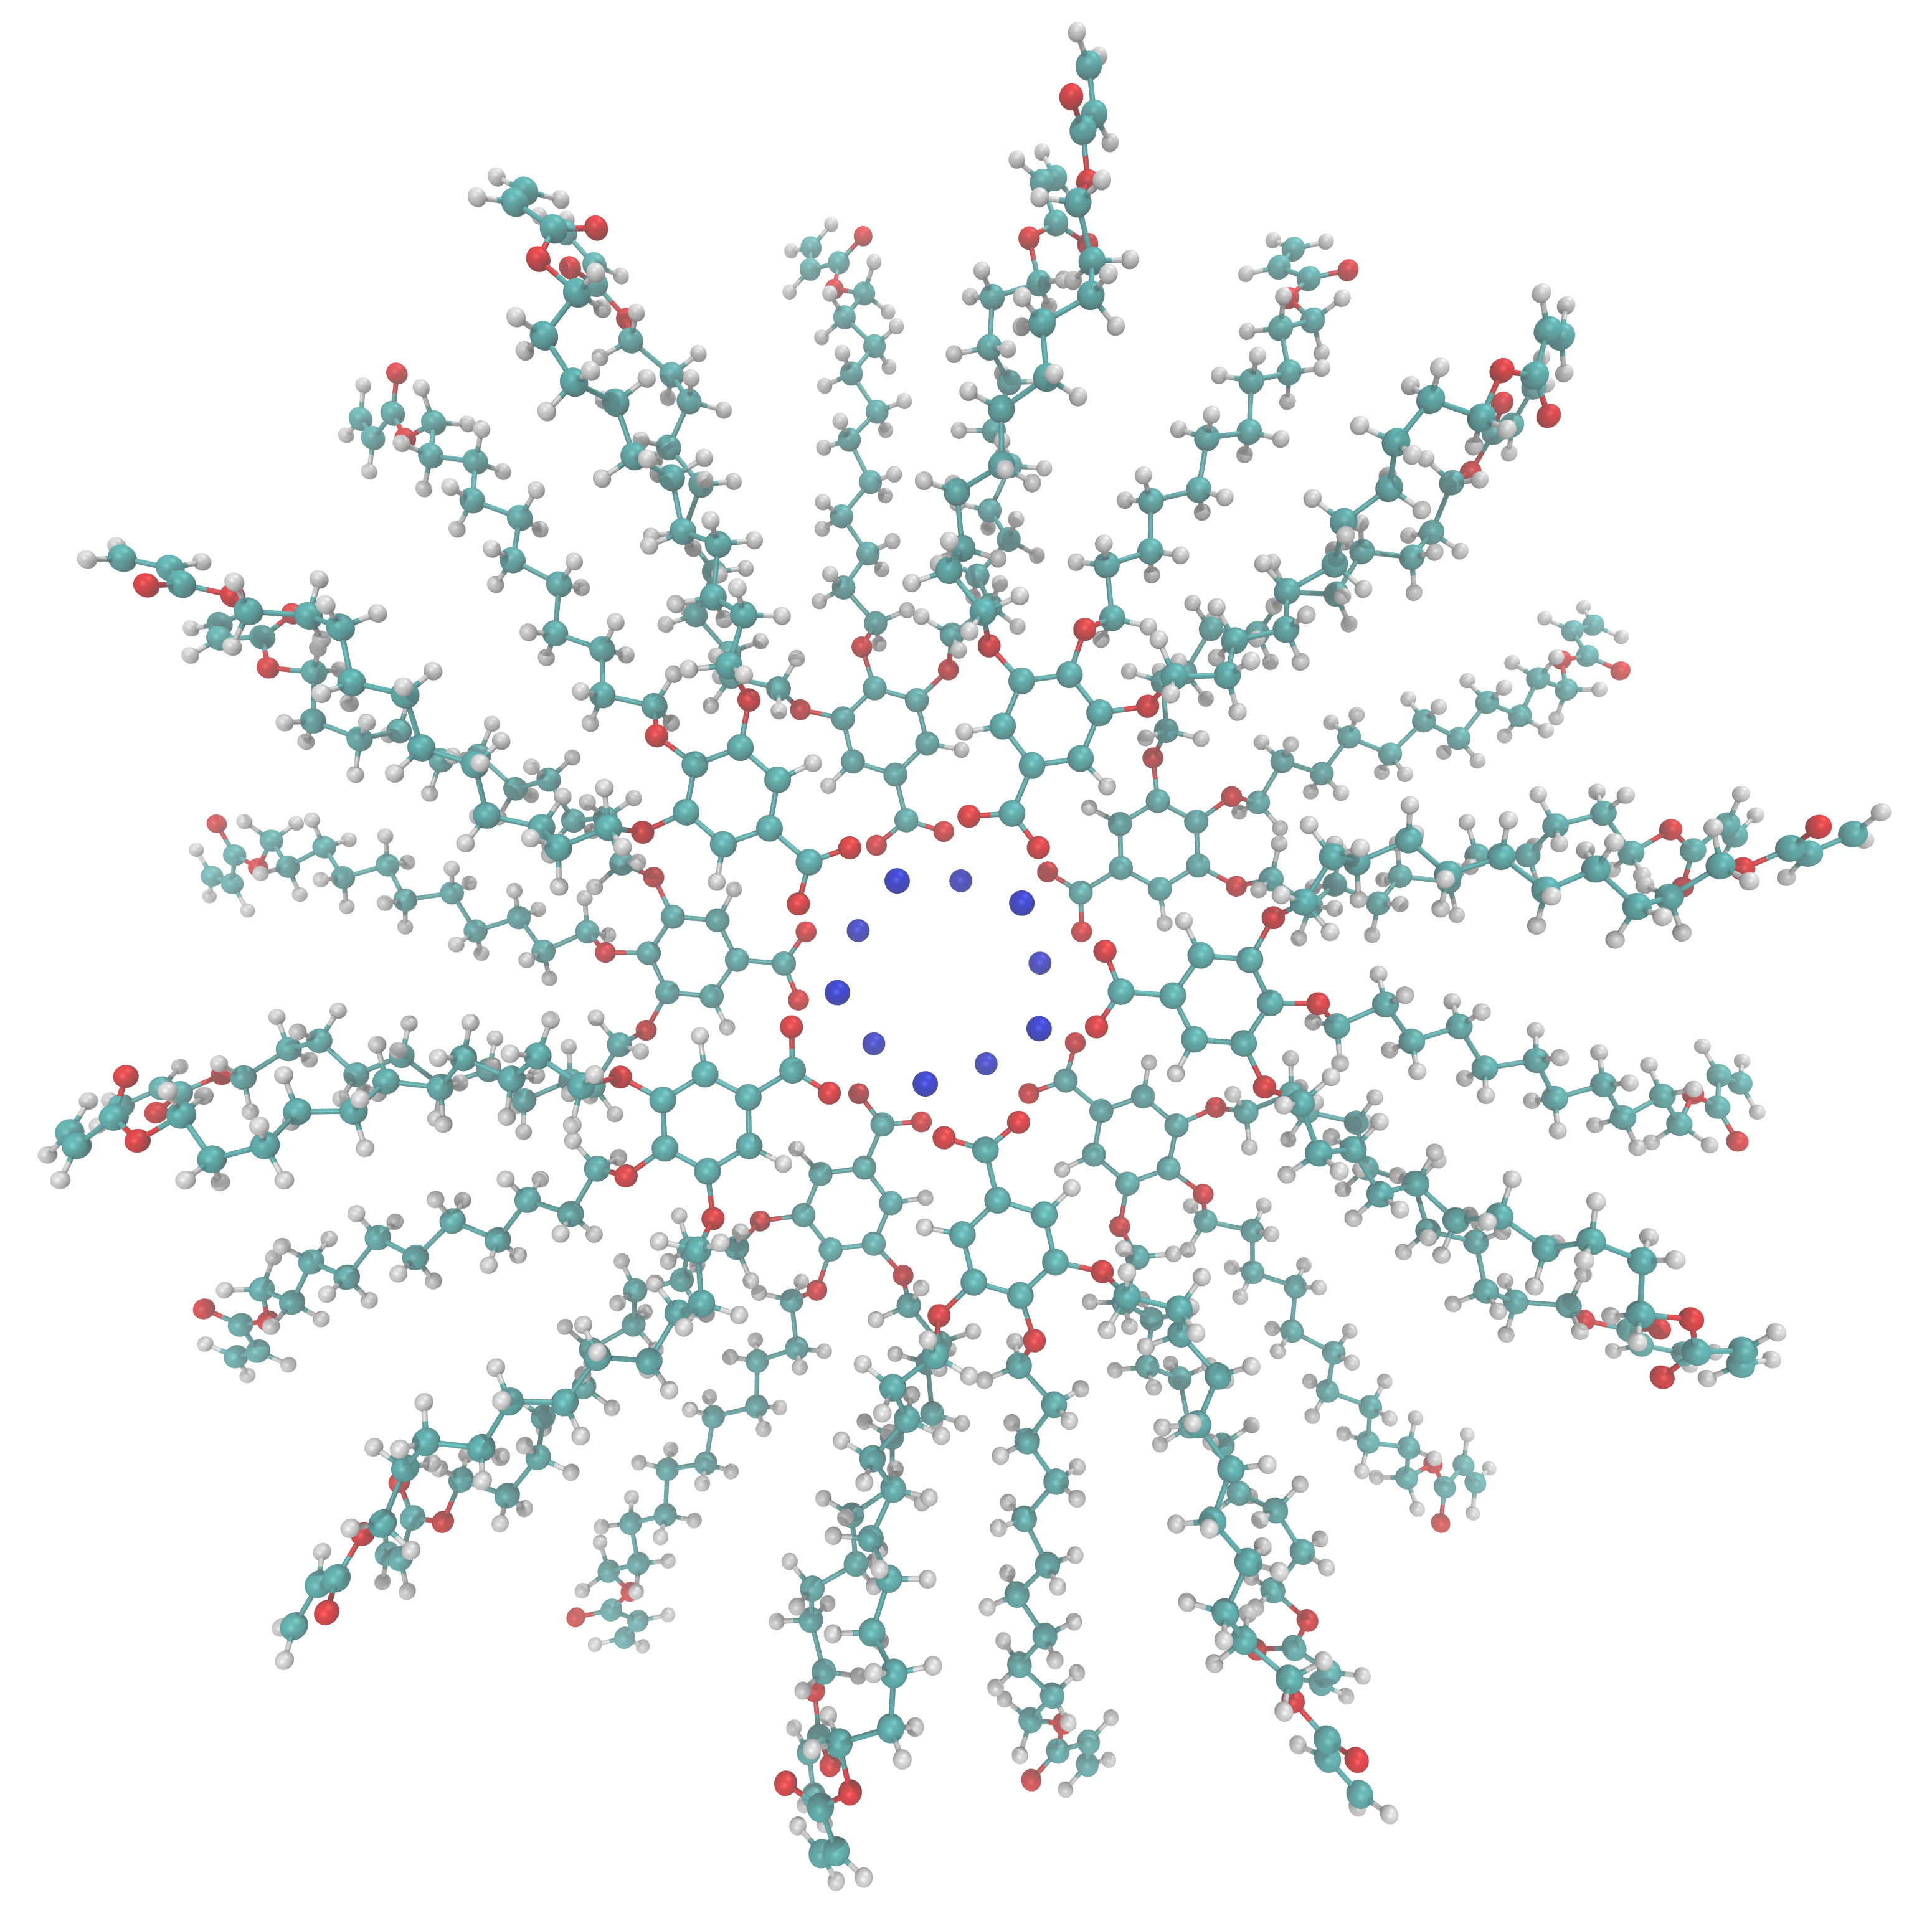
\includegraphics[width=\textwidth]{offsetlayers.png}
		\caption{}\label{fig:offsetlayers}
	\end{subfigure}
	\caption{(a) Sandwiched benzene dimers stack 3.8 \angstrom~apart. (b) Parallel-Displaced benzene dimers stack
	3.4 \angstrom~vertically and 1.6 \angstrom~horizontally apart. (c) T-shaped benzene dimers stack 5.0 \angstrom~apart. 
	(d) Two monomer layers stacked in the sandwiched configuration (e) Two monomer layers stacked in the parallel-displaced
	configuration }\label{fig:stacking}
  \end{figure}
  
  We explored the pore composition by measuring the average number densities of
  various monomer components with respect to the pore centers.
  \begin{itemize}
	\item The centers of the pores were located using the same method to
        calculate the equilibrium pore spacing
        \item We looked at the average number density of sodium ions, aromatic
	rings and carbon atoms making up the monomer tails 
	\item The radial distance from the pore center of all atoms in each group
        are binned then normalized by area 
	% Maybe write an equation here? It's hard to say precisely how I did it in words without it sounding confusing 
  \end{itemize}

  We calculated ionic conductivity using two different methods for robustness.
  \begin{itemize}
    \item The Nernst-Einstein relation relates the DC ionic conductivity to 
    ion diffusivity, $D$, concentration, $C$, ion charge, $q$, the boltzmann 
    constant, $k_b$, and temperature, $T$: $$\sigma = \dfrac{q^2CD}{k_b T}$$  %BJC: need citation
    \item Sodium ion diffusion coefficients were found by calculating the slope
    of the linear region of the z-direction mean square displacement curve as indicated by
    the einstein relation \cite{einstein_investigations_1956}.]
    %MRS: state how you decided which was the linear region.
    %BJC: nothing fancy other than looking at the msd plot and determining where to
    % start fitting. I suppose I could minimize R^2 but that seems like overkill
    \item We looked at the MSD plot to determine where to begin and end a linear fit
    \item Ion concentration was measured with respect to the entire unit cell. 
    % new paragraph
    \item The second method, termed the 'Collective Diffusion' model, measures 
    the movement of the collective variable, Q, which is defined as the amount
    of charge transfer through the system and can be thought to represent
    the center of charge of the system.
    \item The conductance, $\gamma$ of the system can be calculated as:
    $$ \gamma = \dfrac{D_Q}{k_b T} $$ Conversion to ionic conductivity is
    achieved by multiplying by channel length and dividing by the membrane
    cross sectional area.
    \item $D_Q$ is the diffusion coefficient of the collective variable Q. It can
    be calculated using the einstein relation.
    \item A full derivation of the model can be accessed elsewhere \cite{liu_collective_2013}.
  \end{itemize}
    
  \section*{Results and Discussion}
  
%  \subsection*{Determination of Nanoscopic Structural Details}
  
  %In order to construct an initial configuration which gives reliable 
  %trends, we need to understand the composition of layers, how far apart
  %to stack the layers, and how to orient them with respect to each other.
  %\begin{itemize
  %	\item To verify our choices for each parameter, we compare our calculations
  %	to experimental small angle X-ray scattering (SAXS), wide angle X-ray
  %	scattering (WAXS), and ionic conductivity measurements.
  %\end{itemize}
  
 % We will now address the questions raised in the introduction in the order
  %that they were asked.  %BJC: Not a fan of this transition

% BJC: How this section (||||) used to be ordered until deciding to put monomers / layer first
%                        VVVV
  %To answer (1), we verified that the system stays partitioned into layers by
  %plotting the pair correlation function calculated between aromatic rings along
  %the length of the pores (Fig~\ref{fig:zdf}).
  % BJC: add how this calculation is done to methods section (put where I talk about
  % choosing distance between layers
  %\begin{itemize}
%	\item Period of fluctuation (layer spacing)
 %       \item Magnitude of fluctuations
%	\item Comment on difference between offset/layered, number of monomers per layer
 % \end{itemize} 	

  % BJC: might replace with a figure containing alllllll of the zdf's
  %\begin{figure}[!ht]
%       \centering
%       \begin{subfigure}{0.45\textwidth}
%               \centering
%               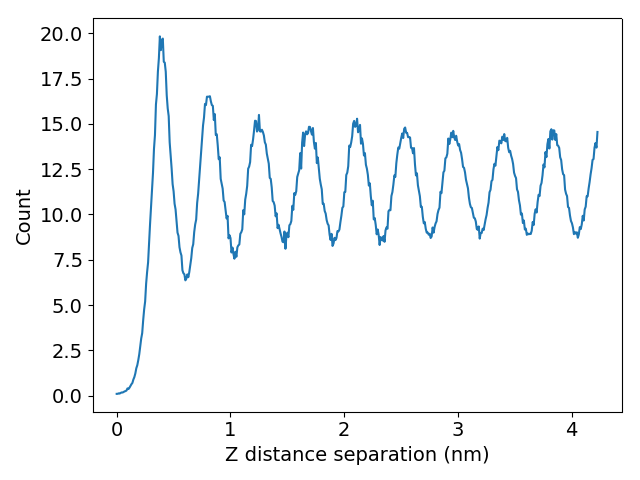
\includegraphics[width=\textwidth]{zdf5layered.png}
%               \caption{}\label{fig:zdf_layered}
%       \end{subfigure}
%       \begin{subfigure}{0.45\textwidth}
%                \centering
%                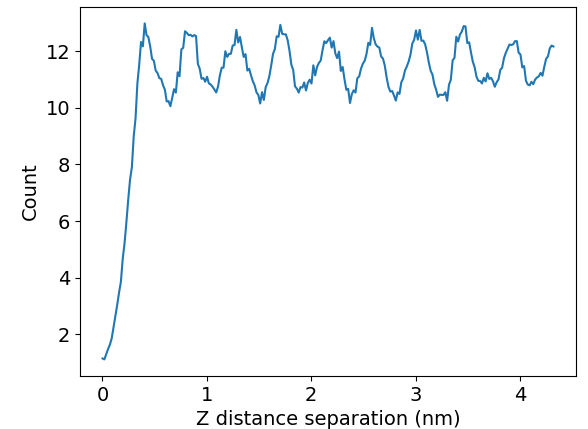
\includegraphics[width=\textwidth]{zdf5offset.png}
%                \caption{}\label{fig:zdf_offset}
%        \end{subfigure}
%        \caption{Pair distribution functions of aromatic carbons for the
%        (a) 5 monomer per layer, sandwiched and (b) 5 monomer per layer,
%        parallel displaced configurations. Clear periodic maxima in the 
%        $z$ probability density indicate distinct layers. The magnitude 
%        of the spikes with respect to the average suggest that the 5 
%        monomer per layer, sandwiched configuration possesses a higher 
%        degree of layer partitioning.}\label{fig:zdf}
%  \end{figure}


%  To discern the composition of the monomer layers, addressing \ref{point:layers}, we ran 
%  simulations of systems created with 4 - 8 monomers per layer.  % BJC: can't figure out how to word this : should be 'with between 4 and 8 monomers' or 'with from 4 to 8 monomers'?  %MRS2: ``with between'', I'd say.
  %\begin{itemize}
%  	\item Both the sandwiched and parallel displaced configurations were tested.
%	\item All systems are stable after 400 ns of simulation.  % BJC: edited this for clarity
        %MRS: you only ran for 50 ns, or after 50 ns some of them started to destabilize?  Is the point you are making that they are ALL pretty stable, or all at least a little stable.   
	%BJC: Working on getting them all run out to 400 ns
%	\item Table ~\ref{table:p2p} shows the pore spacing for all systems tested. 
%	\item Systems built with 5 monomers in each layer equilibrate to a pore spacing
%	that is most consistent with the experimental value of 4.12 nm derived from
%	SAXS measurements (Figure~\ref{fig:SAXS}).
%	\item The remainder of this discussion will focus on the analysis of systems
%	built with 5 monomers per layer. 
%  \end{itemize}

%MRS2: suggest starting with conclusion.  Something like ``The simulations best support the model of 5 monomers per layer based on the pore-to-pore distances.'' Then provide evidence. Suggest for all points.

  \subsection{Density of monomers around pores}
  %MRS4: Perhaps instead of talking about ``layers'', we can talk about axial density correlations.  You can say that for the simulated systems, they appear to stay in highly ordered layers, but that the density correlations are low enough that layering is likely not a clear enough description.  
  %BJC4: Can I support this by plotting the density of head groups axially and show that the peaks are wide/noisy?
  Our simulations best support a model built with 5 monomers per layer based on
  the measured equilibrated pore-to-pore distances. To discern the composition of
  the monomer layers, addressing question (\ref{point:monomernum}), we ran
  simulations of systems created with 4--8 monomers per layer. 
  \begin{itemize}  
  		\item We built systems in both the parallel displaced and sandwiched configurations and
  		equilibrated them according to the dry equilibration procedure.
  		\item We test all systems with an initial layer spacing, l, of 3.7 \AA.
  		\item We tested 4 additional systems with layers initially spaced 5 \AA~apart (See 
  		supporting info for more details on sensitivity to initial layer spacing)
  		\item The pore-to-pore spacing is stable in all systems after 400 ns of simulation. 
  		Figure~\ref{fig:p2p} shows the equilibrated pore-to-pore distances for all systems 
  		tested. 
  		\item Systems built with 5 monomers in each layer equilibrate to a pore spacing that is 
  		most consistent with the experimental value of 4.12 nm derived from SAXS measurements 
	    (Figure~\ref{fig:SAXS}).
	    \item comment about disordered systems
  \end{itemize}
  
  %  The simulations best support a model built with 5 monomers per layer based on 
%  the measured pore-to-pore distances. To discern the composition of the monomer 
%  layers, addressing (\ref{point:monomernum}), we ran simulations of systems created
%  with 4 - 8 monomers per layer.  % BJC: can't figure out how to word this : should be 'with between 4 and 8 monomers' or 'with from 4 to 8 monomers'?
%  \begin{itemize}
%        \item We created systems in both the parallel displaced and sandwiched configurations
%	\item All systems were prepared according to the dry equilibration procedure
%        \item All systems are stable after 400 ns of simulation.  
%        \item Figure ~\ref{fig:p2p} shows the pore spacing for all systems tested.
%        \item Systems built with 5 monomers in each layer equilibrate to a pore spacing
%        that is most consistent with the experimental value of 4.12 nm derived from
%        SAXS measurements (Figure~\ref{fig:SAXS}).
%        \item The remainder of this discussion will focus on the analysis of systems
%        built with 5 monomers per layer.
%  \end{itemize}

  The remainder of this discussion will focus on the analysis of systems built with
  5 monomers per layer. 
  \begin{itemize}
	  	\item Systems built with 6 monomers per layer have an equilibrated
  		pore spacing c.a. 0.50 nm higher than experiment. 
  		\item Systems built with 4 monomers per layer equilibrate to a pore spacing 0.25 nm 
  		lower than experiment. 
  		\item In a sense, all systems tested are at least metastable, however not all will make 
  		physical sense or fit the experimental profile that we are trying to match.
  		\item In the limit of infinite simulation time, all simulations will converge to a 	
  		single density.
  		\item It is our intention to choose an initial configuration which quickly reaches a 
  		monomer density close to experiment.
  \end{itemize} 

  % BJC4: I will add 6 mon/layer disordered data once I have it. The 6 mon/layer I have was
  % equilibrated differently (layers initially spaced 10 \AA apart and jumped straight into
  % npt), and only for sandwiched config. I have parallel displaced and sandwiched 6mon/layer
  % running currently.
  \begin{figure}
	\centering
	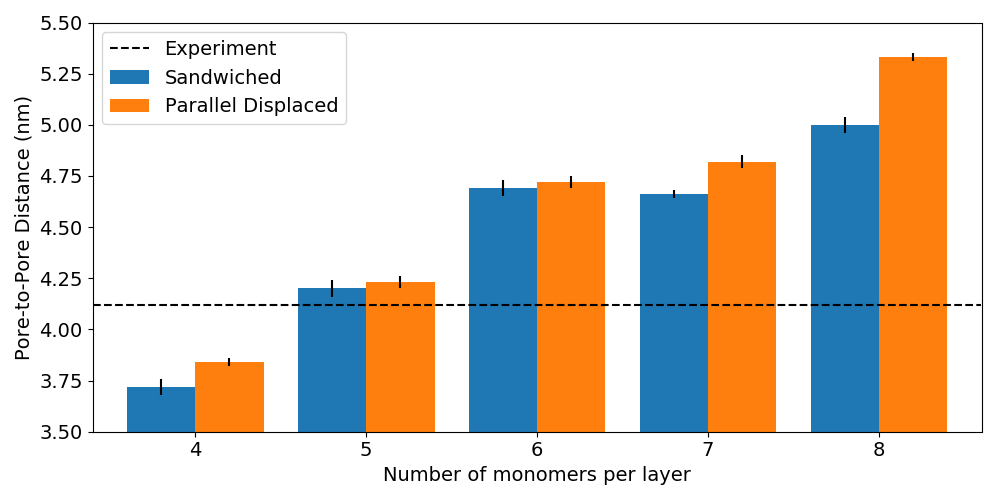
\includegraphics[width=\linewidth]{p2p.png}
	\caption{Systems with 5 monomers per layer have equilibrated pore spacings closest to
			 the experimental value of 4.12 nm, regardless of initial layer spacing, l. The 
			 equilibrated pore spacing of the model increases as the number of monomers 
			 in each layer increases. The pore spacing of systems starting in the sandwiched 	
			 configuration are systematically lower than those started in the parallel 
			 displaced configuration.}~\label{fig:p2p}
  \end{figure}

% BJC3: replaced by plot above.
%  \begin{table}[h]
%  \centering
%  \begin{tabular}{ccc}
%  \toprule
%  		   & \multicolumn{2}{c}{Starting Configuration} \\
%  \hline
%  Monomers per layer & Sandwiched & Parallel Displaced \\
%  \midrule
%  4 & $3.72 \pm 0.04$ & $3.84 \pm 0.02$ \\  % done
%  5 & $4.20 \pm 0.04$ & $4.23 \pm 0.04$ \\
%  6 & $4.69 \pm 0.04$ & $4.72 \pm 0.03$ \\
%  7 & $4.66 \pm 0.02$ & $4.82 \pm 0.03$ \\  % done
%  8 & $5.00 \pm 0.04$ & $5.33 \pm 0.02$ \\
%  \bottomrule
%  \end{tabular}
%  \caption{The pore spacing (given in nm) of the model increases as
%  number of monomers in each layer increases. The pore spacing of a system
%  starting in the sandwiched configuration is systematically lower than 
%  that started in an offset configuration. Systems built with 5 monomers
%  per layer in a parallel displaced configuration result in a pore spacing
%  closest to the experimental 4.12 nm}
%  \label{table:p2p} 
%  \end{table}

  \subsection{Structural determination}
  
  We further refined our structural understanding of the system by simulating X-ray 
  diffraction patterns produced from equilibrated MD trajectories and comparing them
  to experiment. 
  \begin{itemize}
	  	\item We tested systems built with 5 monomers per layer in the parallel 
		displaced and sandwiched configurations at 300 K with layers initially spaced
		3.7 \AA~and 5.0 \AA~apart.
		\item We generated simulated patterns using portions of simulation trajectory
		after equilibration.
		\item The patterns for all structures are shown and compared to experiment
		in Figure~\ref{fig:XRDsim}.
  \end{itemize}

%  Simulated XRD of the sandwiched configuration contains all experimental
%  features except for R-double. R-alkanes, R-spots and R-pores appear close to their
%  expected locations. R-$\pi$ is also present, however it intersects R-alkanes at
%  a $q_z$ value lower than experiment meaning the head groups in our model prefer 
%  to stack farther apart. 

%  Like the sandwiched configuration, the parallel displaced configuration creates
%  a simulated XRD pattern with all major experimental reflections except for R-double.
%  R-alkanes and R-pores appear as they do in the sandwiched configuration. R-spots
%  and R-$\pi$ appear, however with a lower intensity
%  relative to R-alkanes when compared to the sandwiched configuration. R-double
%  appears due to the parallel displaced aromatic rings. It is a subharmonic of
%  R-$\pi$ since the nearest vertically stacked head group to any given head group
%  is $2\times$R-$\pi$~away. 
% BJC: adjust figure size and alignment -- probably easiest to set figure size in matplotlib
  
%BJC4: I'm not sure what the best way to set up this figure is yet.
  \begin{figure}[htb]
	\centering
	\begin{subfigure}{0.4\linewidth}
	\centering
			\begin{subfigure}{\textwidth}
		       		\centering
	        		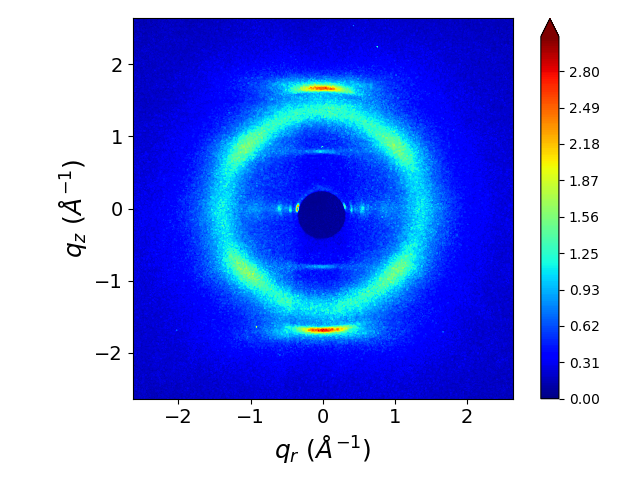
\includegraphics[width=\linewidth]{WAXS_raw_jet.png}
	        		\caption{Experimental WAXS}~\label{fig:offset_tails}
			\end{subfigure}
	\end{subfigure}
	\begin{subfigure}{0.28\linewidth}
			\begin{subfigure}{\textwidth}
			\centering
		        	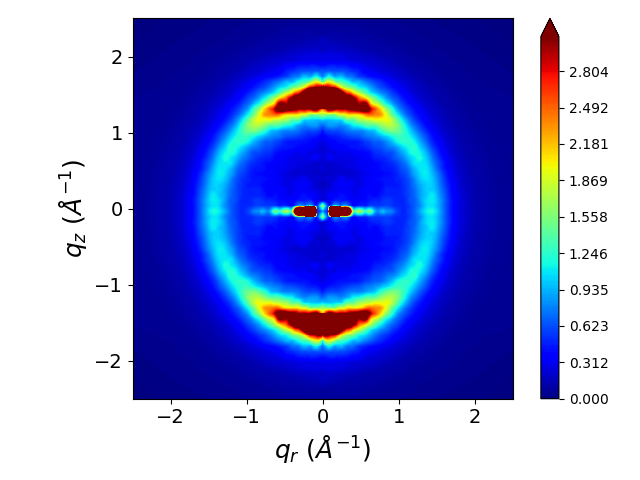
\includegraphics[width=\linewidth]{rzplot_layered_300K_jet.png}
			        \caption{Sandwiched}~\label{fig:rzplot_layered_300K}
			\end{subfigure}
			
			\begin{subfigure}{\textwidth}
		       		\centering
	        		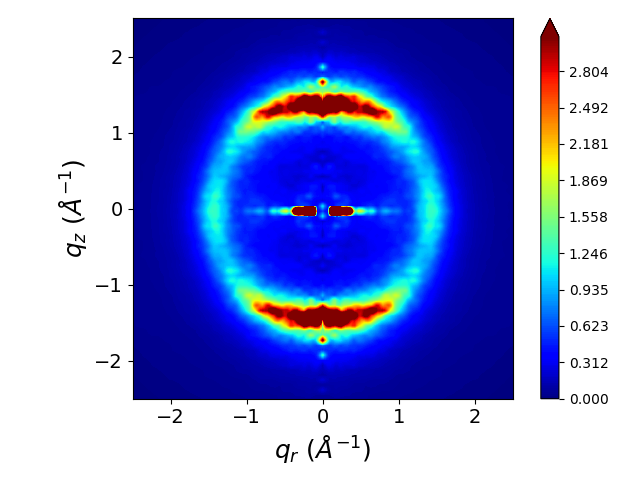
\includegraphics[width=\linewidth]{rzplot_layered_300K_disorder_jet.png}
	        		\caption{Disordered sandwiched}~\label{fig:rzplot_layered_300K}
			\end{subfigure}
	\end{subfigure}
	\begin{subfigure}{0.28\linewidth}
	\centering
			\begin{subfigure}{\textwidth}
			\centering
		        	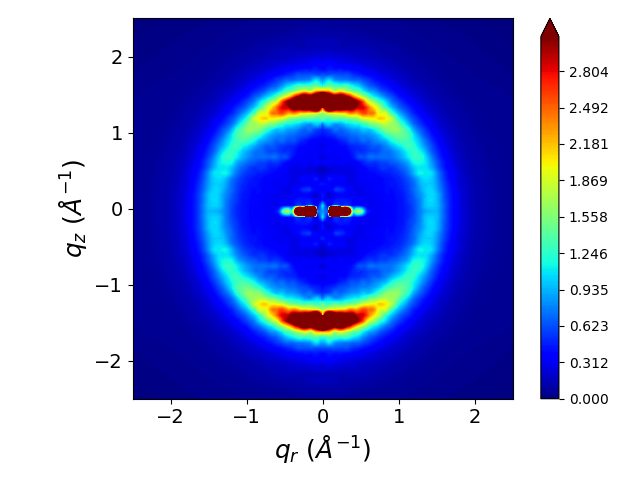
\includegraphics[width=\linewidth]{rzplot_offset_300K_jet.png}
			        \caption{Parallel displaced}~\label{fig:rzplot_offset_300K}
			\end{subfigure}
			
			\begin{subfigure}{\textwidth}
			\centering
		        	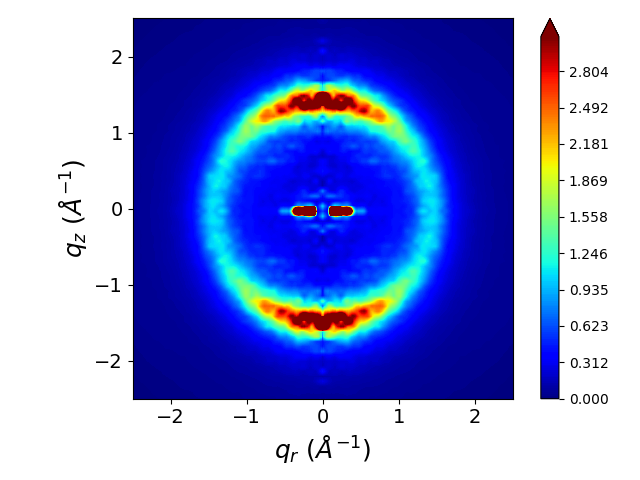
\includegraphics[width=\linewidth]{rzplot_offset_300K_disorder_jet.png}
			        \caption{Disordered parallel displaced}~\label{fig:rzplot_offset_300K_disordered}
			\end{subfigure}
	\end{subfigure}
	\caption{Very descriptive caption}~\label{fig:XRDsim} 
	\end{figure}

  The simulated XRD patterns produced from both systems show moderate qualitative 
  agreement with experiment. 
  \begin{itemize}
  		\item R-alkanes and R-pores appear in the expected location
    %MRS4: we will need to provide more details: more intense is just qualiatative.
    %BJC4: I can include the intensity of the first peak of R-pores in the tables that 
    % show relative intensities.
  		\item R-pores is more intense than experiment, likely because we are simulating a 
		perfect, infinite hexagonal array. The real system has defects and domain misalignment
	    which decreases the overall intensity.
    %MRS4: comments from Matt suggest that domain misaligment shouldn't alone be responsible for the difference in intensity ratio. Some of the experiments should help explain it better. Let's talk!
    %BJC4: So a combo of: domain misalignment, defects, slow dynamics of simulated system, only 4 
    %pores in unit cell, tortuosity (?)
    %MRS5: maybe, there's a question of how we can demonstrate the magnitude of any of these effects.
    	\item R-spots appears to be weaker in the simulated patterns. They are also partially 
	    engulfed by the wide R-$\pi$ reflection.
	    \item We further explore R-spots in Section~\ref{section:rspots}  
        \item R-$\pi$ appears at a lower $q_z$ value than experiment. In all systems, the
	    reflection reaches its maximum at $q_z < 1.5 \AA^{-1}$ which means that monomers
	    prefer stack greater than 4.2 \AA~apart rather than 3.7 \AA. This behavior is not
	    surprising since GAFF models atoms as point charges and does not appropriately model 
	    the aromatic $\pi-\pi$ interactions which would cause the monomers to stack closer
	    together.
	    \item We will explore R-$\pi$ in more detail in Section~\ref{section:rpi}.
            %MRS4: interesting that the main pi-pi stacking follows the isotropc alkane curve so significantly.
			%BJC4: Might have something to do with the distibution of tilt angles in the tails
	    \item R-double does not appear in any of the patterns
	    \item We will explore its possible origins and reasons that it does not appear in our
	    simulated patterns in Section~\ref{section:rdouble}.
  \end{itemize}
  
  The simulated XRD pattern of the parallel displaced configuration shows an additional
  reflection due to its helical structure. 
  \begin{itemize}
  		\item There are horizontal reflections at $|q_z|= 0.7~\AA^{-1}$, exactly half of 
  		the $q_z$ value of R-$\pi$. 
  		\item The reflection does not cross through $q_r = 0~\AA^{-1}$ so it does not
  		appear for the same reason as R-double. 
  		\item This type of pattern is characteristic of a helix (reference something)
  		\item It is possible that these reflections contribute to the continuation of
  		R-double into R-alkanes, as seen in the experimental pattern. 
  \end{itemize}
  
  %BJC4: This paragraph might fit better before qualitative description
  We quantified the numerical discrepancies present when comparing the relative intensities
  of each reflection of interest between experimental and simulated patterns. 
  \begin{itemize}
  		\item Table~\ref{table:relative_inensities_300K} quantifies the relative intensity
  		of each reflection for each system tested.
  		\item The patterns are normalized so that the average intensity of R-alkanes equals 1. 
  		% BJC4: I need to explain how I calculated these intensities somewhere. Is this the right
  		% place to do it? I think it would just be confusing in the methods. I could also move it
  		% to supplemental.
  		\item We measured the approximate intensity of R-$\pi$ by measuring the intensity of 
  		the peak of the cross-section at $q_r=0$. 
  		\item The relative intensity of R-$\pi$ is significantly higher than experiment in our
  		simulations.
  		\item R-spots is measured as the average intensity within the region bounded by a 'spot'.
  		Spots are identified based on visual inspection. If there is no easily discernable spot,
  		then the intensity is taken as that of the intersection of R-alkanes at half the $q_z$
  		value of R-$\pi$, since that is where it appears experimentally. 
  		\item The intensity of R-spots is slightly lower than experiment in all cases.
  		\item There is no R-double intensity to be measured.
  \end{itemize} 

  \begin{table}[h]
  \centering
  \begin{tabular}{cccccc}
  \toprule
  		   & \multicolumn{5}{c}{Configuration} \\
  \hline
  Reflection & Experiment & Sandwiched & Parallel Displaced & Disordered Sandwiched & Disordered Parallel Displaced \\
  \midrule
  R-alkanes & 1.0 &  1.0 &  1.0 & 1.0 & 1.0  \\  
  R-spots   & 1.3 &  1.2 &  1.2 & 1.2 & 1.2  \\
  R-$\pi$   & 2.8 & 18.1 & 14.2 & 7.8 & 10.0 \\
  R-double  & 0.9 &  --  & --   &  -- & --   \\ 
  \bottomrule
  \end{tabular}
  \caption{The simulated XRD patterns of the systems tested, normalized so that the average 
  intensity of R-alkanes equals 1, show R-$\pi$ reflections that are significantly higher 
  than experiment and R-spots reflections that are slightly lower than experiment. R-double
  does not appear in any patterns, and thus has no measurable intensity.}
  \label{table:relative_inensities_300K} 
  \end{table}
%MRS5: just numberwise, the disordered seem to match better. If we don't think those are right, will have to provide some additional reasoning.

%  The simulated XRD pattern produced from the sandwiched configuration is missing
%  R-double and R-spots. 
%  \begin{itemize}
%		\item R-pores and R-alkanes appear in their expected locations. 
%		\item R-pores is more intense than experiment, likely because we are simulating a 
%		perfect, infinite hexagonal array. The real system has defects and domain misalignment
%	    which decreases the overall intensity.
%	    \item R-$\pi$ appears with a very high intensity and is shifted down to a lower value
%	    of $q_z$ meaning monomers in our model prefer to stack farther apart.  
%	    \item R-spots may be faintly present, however it is not present to the degree shown
%	    experimentally. (see table with relative intensities) 
%  \end{itemize}

  %BJC: discussed parallel displaced and sandwiched configs in separate paragraphs to 
  % avoid confusion. Need to make thesis less dry. 
%  The simulated XRD pattern generated from the parallel displaced configuration is also
%  missing R-double and R-spots.
%  \begin{itemize}
%  		\item R-pores and R-alkanes appear in the expected location again
%  		\item R-$\pi$ is present in the same location as the sandwiched configuration with
%  		high intensity. 
%  		\item R-double is not present, however off-axis reflections appear at the same value 
%  		of $q_z$ where we expect to see R-double. These appear since there is a helical 
%  		arrangement of monomers in the parallel displaced configuration. A helix alone will
%  		not give rise to a reflection at $q_r = 0$ (See supporting info for demonstration)
%  		\item There is elevated intensity where we expect to see R-spots, however it cannot
%  		be easily distinguished from the higher intensity arcs which overlay the top and 
%  		bottom of R-alkanes.
%  \end{itemize}

  There are clear differences between our simulated results and experimental results
  that must be addressed and justified. We will explore the origin of each experimental 
  reflection and form structural hypotheses related to their appearance in our simulated 
  patterns. Specifically, we want answer:  
  \begin{enumerate}
	\item What is the origin of R-spots?
  	\item Why is the intensity of R-$\pi$ so much greater than experiment?
  	\item What is the origin of R-double?
  \end{enumerate}

  \subsubsection{Origin of R-spots}\label{section:rspots}

  We observe an increase in the intensity of R-spots when we simulate systems at 280K. 
  \begin{itemize}
  		\item R-spots is most intense in the sandwiched configuration
  		(Figure~\ref{fig:sandwiched280K}).
  		\item The relative intensity of R-spots is higher than in experiment (1.5 vs. 1.3) 
  		\item Still no R-double
  		%BJC4: I think the following is a reasonable thing to do. Use a configuration that really
  		% exhibits R-spots so we can definitively (as best as possible anyways) prove its origin. 
  		% Otherwise, we will have to go off the 300K data which isn't as clear cut. 
  		\item We can use this configuration to more thoroughly explore the origin of R-spots.
  \end{itemize}
  
  \begin{figure}
	  \begin{subfigure}{0.45\linewidth}
	  	\centering
	  	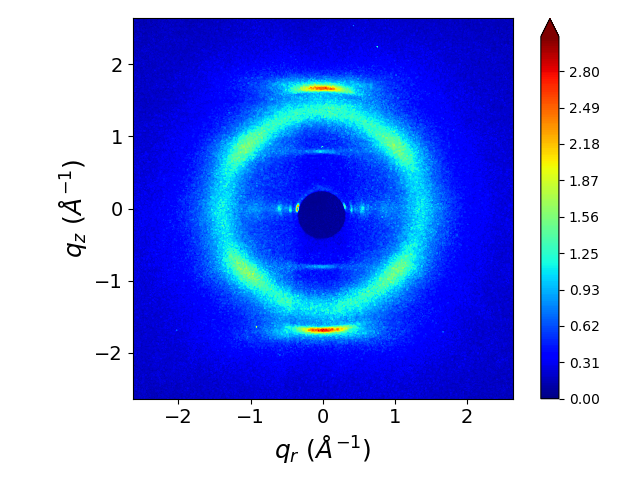
\includegraphics[width=\linewidth]{WAXS_raw_jet.png}
	  	\caption{}
	  \end{subfigure}
	  \begin{subfigure}{0.45\linewidth}
	  	\centering
	  	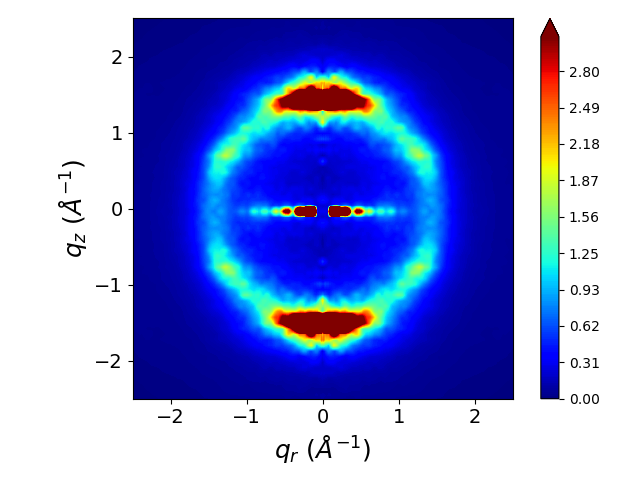
\includegraphics[width=\linewidth]{rzplot_layered_280K_jet.png}
	  	\caption{}\label{fig:sandwiched280K}
	  \end{subfigure}
  \caption{R-spots increases in intensity when the temperature of the system is lowered to 280K.
  In this case, the simulated R-spots is more intense than experiment.}
  \end{figure}
  
  % %BJC3: update with 300K pics. Presented separately from 280K for now. 
%  \begin{figure}
%  \begin{subfigure}{0.3\linewidth}
%        \centering
%        \vspace{-0.2em}
%        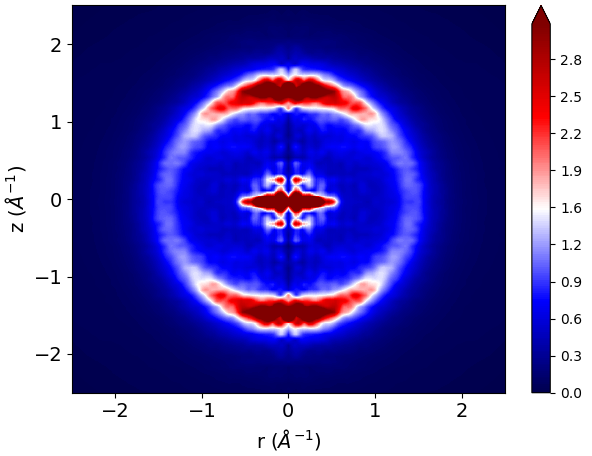
\includegraphics[width=1.1\linewidth,trim={1cm 0 1.3cm 0},clip]{rzplot_offset_300K.png}
%        \caption{}~\label{fig:rz_offset}
%  \end{subfigure}
%  \begin{subfigure}{0.3\linewidth}
%        \centering
%        \vspace{0.25em}
%        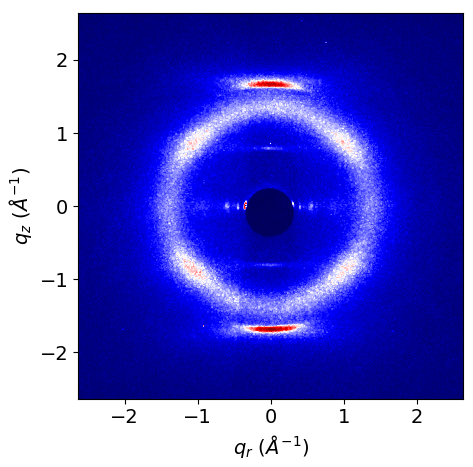
\includegraphics[scale=0.285]{WAXS_raw.png}
%        \caption{}~\label{fig:raw_waxs}
%  \end{subfigure}
%  \begin{subfigure}{0.3\linewidth}
%        \centering
%        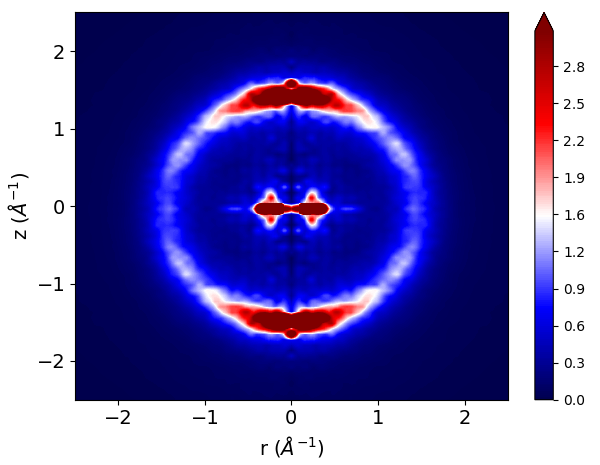
\includegraphics[width=1.1\linewidth,trim={1cm 0 1.3cm 0},clip]{rzplot_layered_300K.png}
%        \caption{}~\label{fig:rz_layered}
%  \end{subfigure}
%  \begin{subfigure}{0.0544\linewidth}
%        \centering
%        \vspace{-4.00em}
%        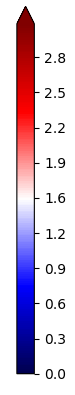
\includegraphics[width=\linewidth]{colorbar_seismic.png}
%  \end{subfigure}
%%MRS6: question: the SAXS region looks different between sandwiched and parallel displaced. Any thoughts why? We can discuss in person.  And seems like have to comment on the difference in intensity between Sandwich and parallel displaced in the pi-pi region.
%%MRS6: I wonder to what extent showing the reflections of tails removed would make it clearer pi-pi is really there.  Maybe in supporting info?
%%BJC2: Sure, I'll add that to supporting info
%%  \caption{The simulated XRD pattern generated from the equilibrated trajectory
%%	  of the parallel displaced configuration (a) exhibits all major reflections
%%	  present in the experimental WAXS pattern (b). The simulated XRD pattern
%%	  generated from the equilibrated trajectory in the sandwiched configuration (c) shows
%%	  all major reflections except R-double.}
%  \label{fig:XRDsim}
%  \end{figure}

  %BJC: might be able to combine with other table
%  \begin{table}[h]
%  \centering
%  \begin{tabular}{cccc}
%  \toprule
%  		   & \multicolumn{3}{c}{Configuration} \\
%  \hline
%  Reflection & Experiment & Sandwiched & Parallel Displaced \\
%  \midrule
%  R-alkanes & 1.0 &  1.0 &   1.0  \\  
%  R-$\pi$   & 2.8 & 27.1 & 119.3  \\
%  R-spots   & 1.3 &  1.6 &   1.2  \\  
%  R-double  & 0.9 &  --  &   --   \\ 
%  \bottomrule
%  \end{tabular}
%  \caption{The relative intensities of reflections of interest}
%  \label{table:relative_inensities_280K} 
%  \end{table}
  
  %BJC3: following taken from draft.tex
  The R-spots signal is not a result of alkane chain tilt. Previous literature
  has attributed the spots in this particular WAXS pattern as the product of tilted alkane
  chains~\cite{feng_scalable_2014}. We looked closer at the sandwiched
  configuration simulated at 280K since R-spots appears with the most strength in 
  its simulated XRD pattern. We measured the tilt angle of the alkane chains and 
  showed that our system equilibrates to an average tilt angle close to zero degrees
  (Fig.~\ref{fig:tilt}). 
  
   %BJC4: include dashed line at mean. 
  \begin{figure}
  \centering
  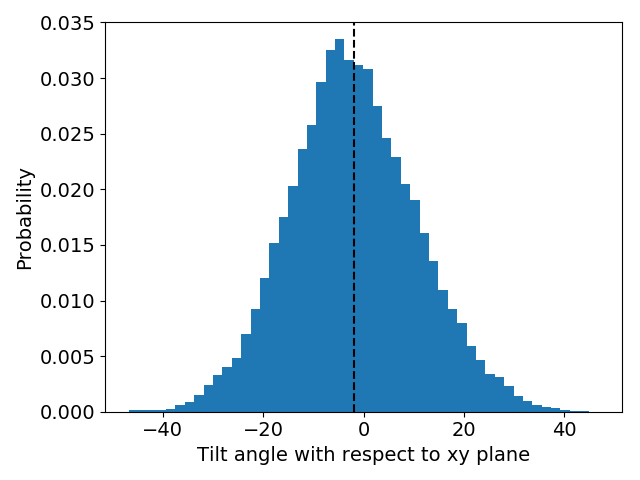
\includegraphics[width=0.5\linewidth]{tilt_dist.png}
  \caption{We measured the angle made between each monomer alkane tail and the
	  membrane plane. The average tilt angle (dashed line) is near -2\degree~which is far from 
	  the 37\degree~tilt angle previously used to explain R-spots.}~\label{fig:tilt}
  \end{figure}

  %BJC3: from draft.tex  
  To understand the origin of R-spots, we determined which
  atoms gave rise to the feature. Since R-spots is present as higher intensity
  spots within R-alkanes, it is likely that the spots arise as a consequence of
  the tails. By removing all non-tail atoms from the trajectory and simulating a
  diffraction pattern with the remaining atoms, we were able to isolate the cause of 
  the spots to the tails (Figure~\ref{fig:tails}). Since the tails stay nearly flat, we plotted
  the centroids of the tails and measured the angle between each centroid and its
  nearest neighbors with respect to the plane of the membrane. We see distinct
  peaks in the distribution of these angles (Figure~\ref{fig:tail_packing}).

%  The peaks in the nearest neighbor angle distribution are consistent with the
%  location of R-spots. The peaks of interest in Figures \ref{fig:offset_tails}
%  and \ref{fig:layered_tails} are located at $\pm 33 \degree$ which is the same
%  location where the highest intensity of spots are located on the simulated
%  patterns. We confirmed this conclusion by radially integrating the 2D WAXS
%  pattern for $\left|\mathbf{q}\right|$ values between 1.4 and 1.57 (between 4
%  and 4.5 \AA~in real space). We observe that distinct peaks appear ca. $30
%  \degree$, in close agreement with the previously measured angle distribution
%  (Figs.~\ref{fig:offset_integration}~and~\ref{fig:layered_integration}). We
%  performed the same integration on the raw experimental data and found the angle
%  at which R-spots reaches its highest intensity to be $\pm 37 \degree$ which
%  is a reconcilable difference with our simulated results.
  
  %BJC: modification of above paragraph to only include 280K sandwiched data
  The peaks in the nearest neighbor angle distribution are consistent with the
  location of R-spots. The peaks of interest in Figure \ref{fig:layered_tails} 
  are located at $\pm 33 \degree$ which is the same
  location where the highest intensity of spots are located on the simulated
  patterns. We confirmed this conclusion by radially integrating the 2D WAXS
  pattern for $\left|\mathbf{q}\right|$ values between 1.4 and 1.57 (between 4
  and 4.5 \AA~in real space). We observe that distinct peaks appear c.a. $30
  \degree$, in close agreement with the previously measured angle distribution
  (Figure~\ref{fig:layered_integration}). We
  performed the same integration on the raw experimental data and found the angle
  at which R-spots reaches its highest intensity to be $\pm 37 \degree$ which
  is a reconcilable difference with our simulated results.

%  The evidence supports the hypothesis that alkane chain tails pack in a
%  hexagonal array. Groups of three tails associated with each monomer prefer to
%  sit between tails of vertically stacked monomers rather than stacking directly
%  on top of them (Figure~\ref{fig:hex_tails}). This type of packing has been seen
%  before in XRD studies of hydrocarbon chains~\cite{small_lateral_1984}.

  \begin{figure}
	\centering
	\begin{subfigure}{0.45\linewidth}
		\centering
	 	\vspace{-2em}
		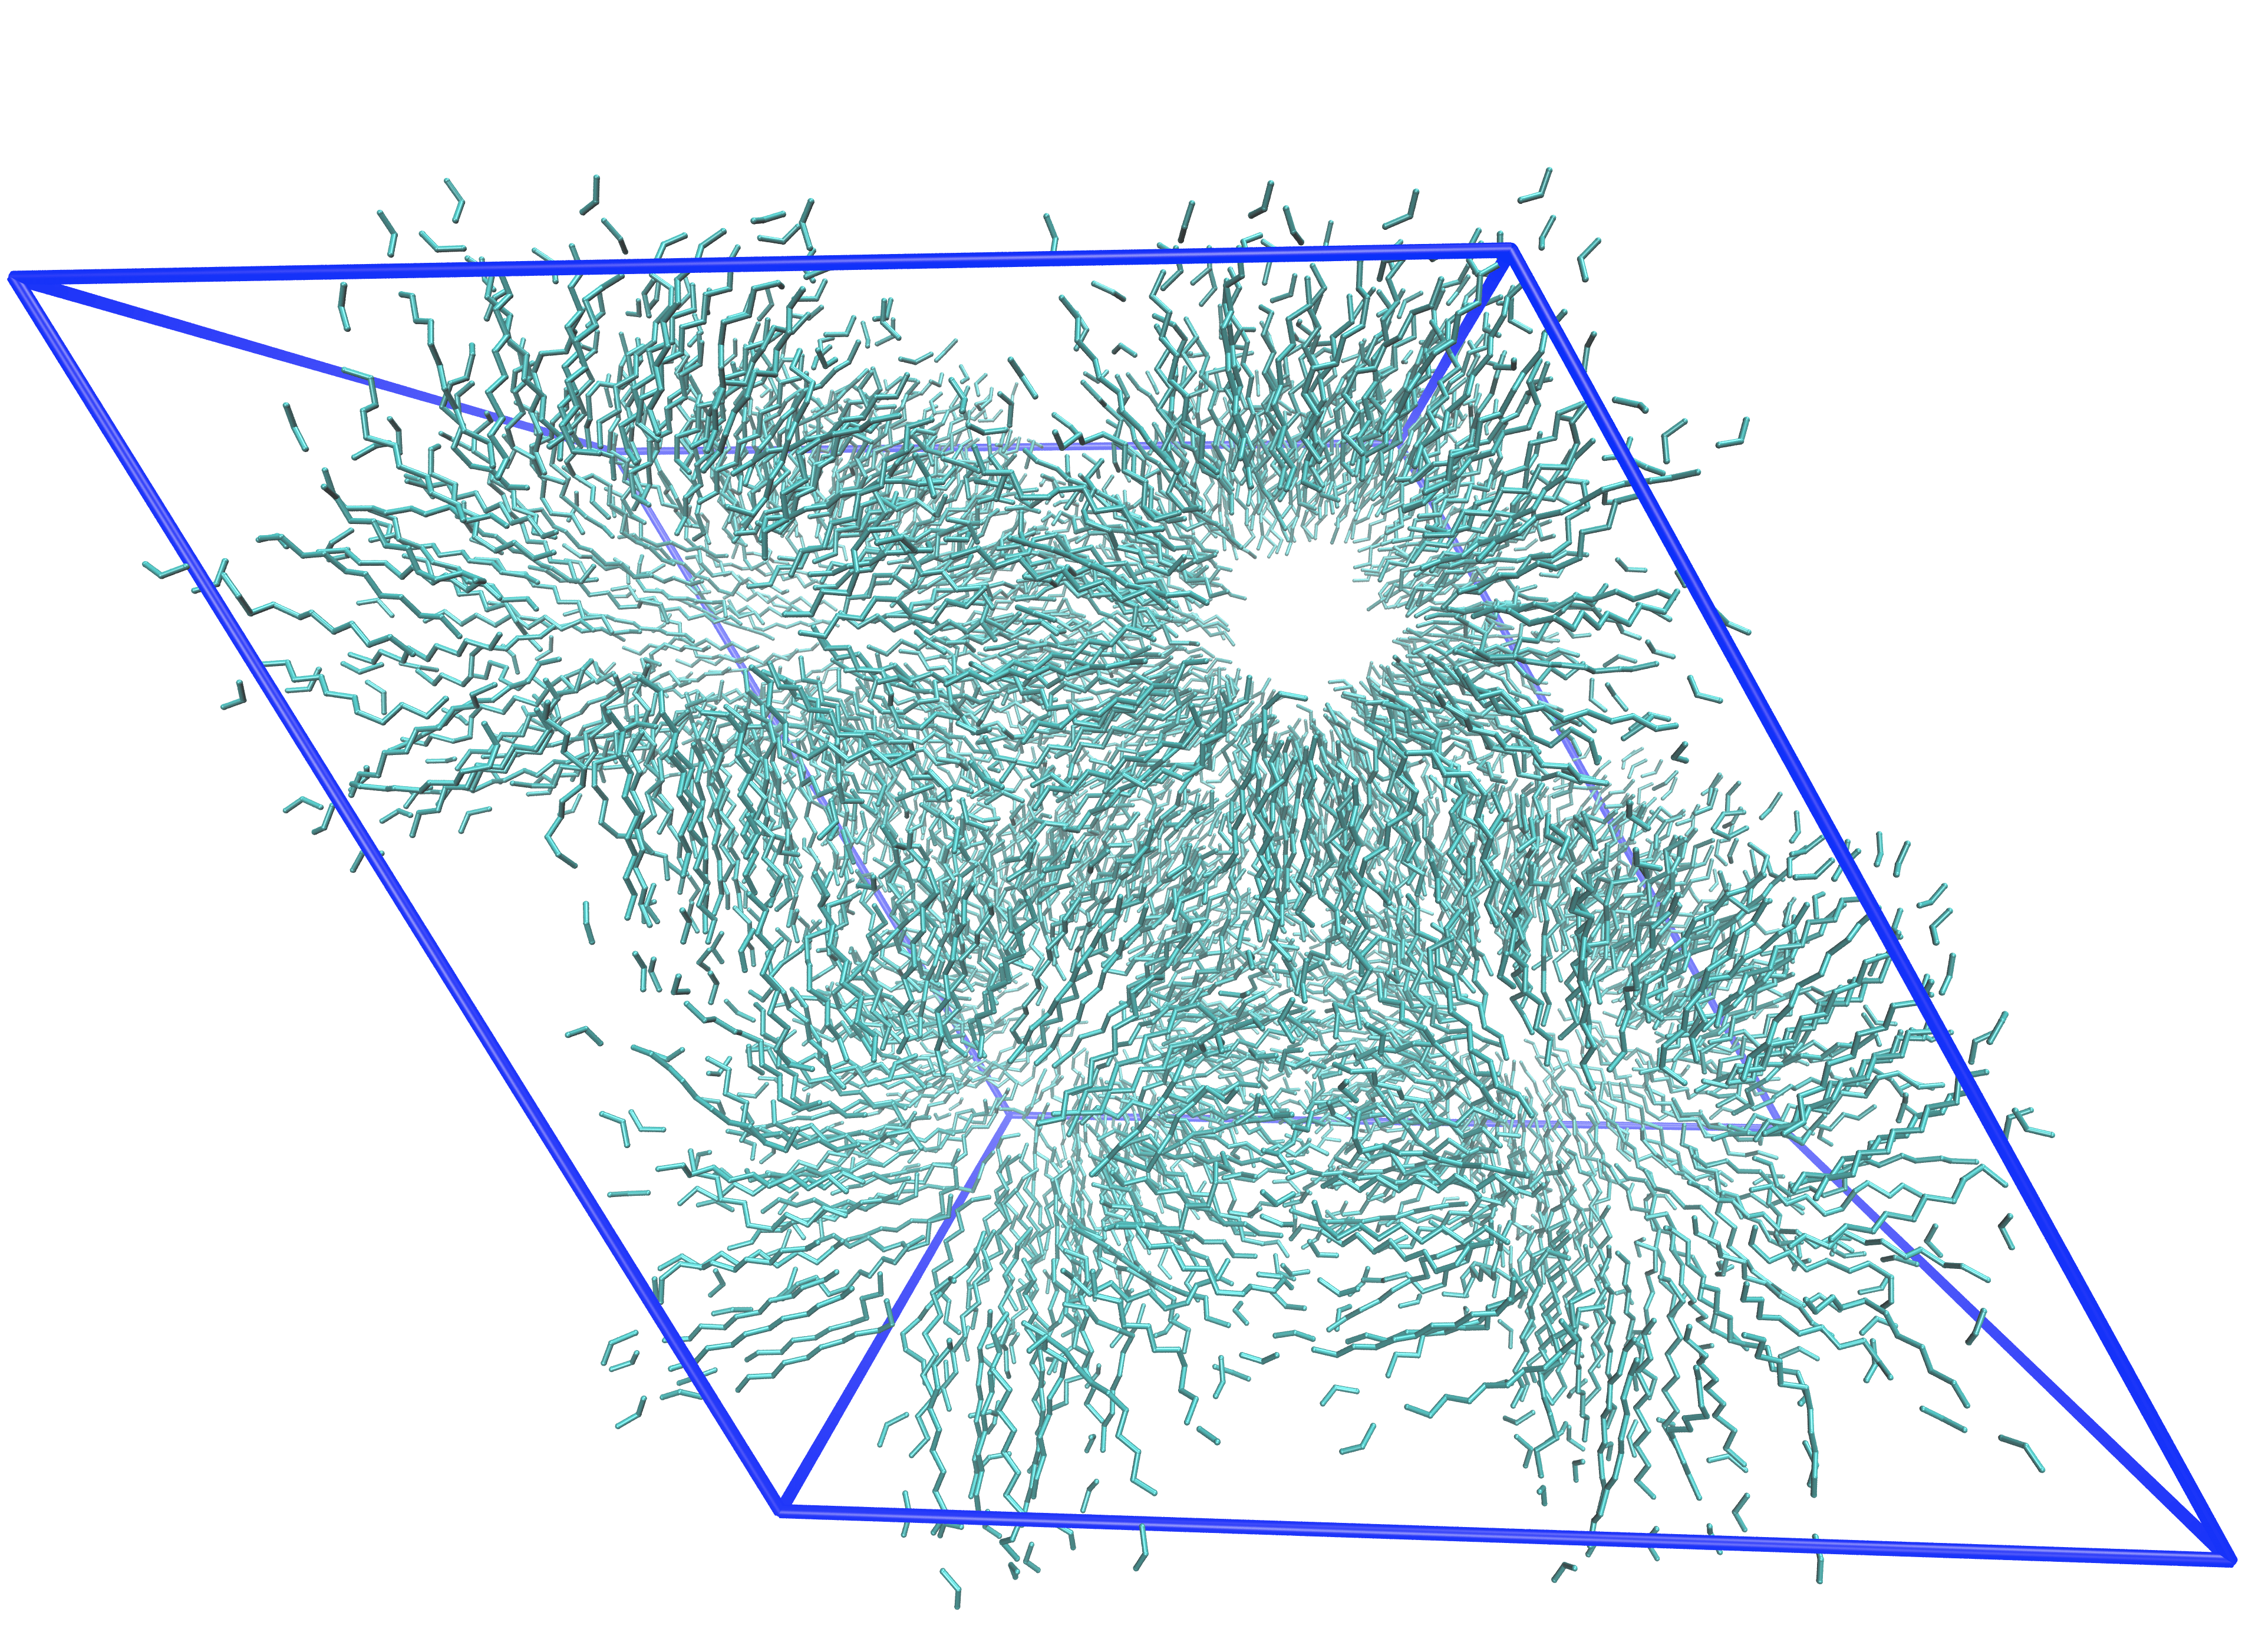
\includegraphics[width=\textwidth]{tails_topview.png}  % picture of top of unit cell with only tail atoms shown
		\caption{}\label{fig:topdown_tails_only}
	\end{subfigure}
	\begin{subfigure}{0.45\linewidth}
		\centering
		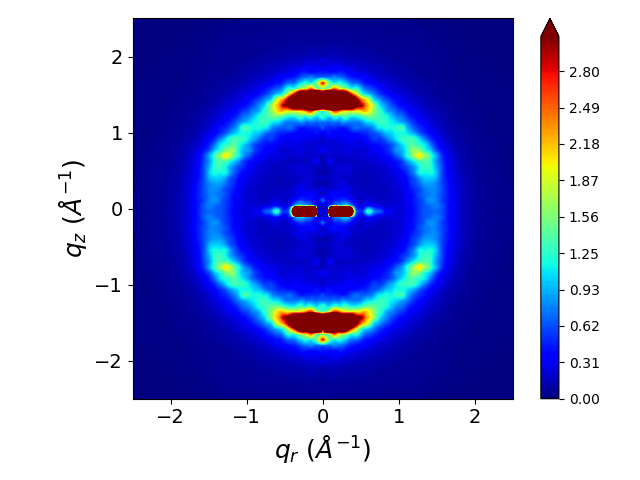
\includegraphics[width=\textwidth]{tails_rzplot_jet.png}
		\caption{}\label{fig:tails_rzplot}
	\end{subfigure}
	\caption{(a) We removed all atoms except carbon atoms that constitute the tails from a 
	sandwiched configuration trajectory. (b) The simulated XRD pattern of the
        tail-only trajectory still shows R-spots}\label{fig:tails}
  \end{figure}

%  \begin{figure}[!htb]
%  \centering
%  	\begin{subfigure}{\linewidth}
%	\centering
%		\begin{subfigure}{0.45\textwidth}
%        		\centering
%        		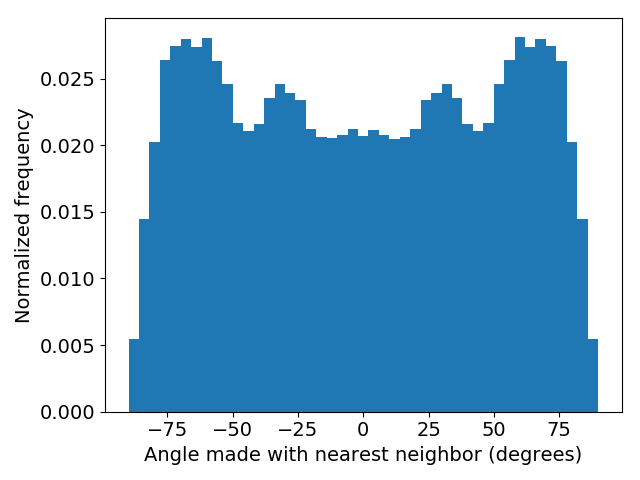
\includegraphics[width=\linewidth]{offset_tail_packing.png}
%        		\caption{}~\label{fig:offset_tails}
%		\end{subfigure}
%		\begin{subfigure}{0.45\textwidth}
%		\centering
%	        	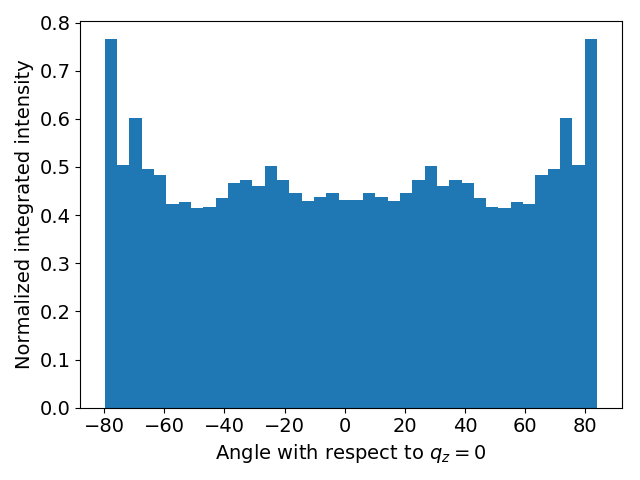
\includegraphics[width=\linewidth]{offset_angle_v_I.png}
%		        \caption{}~\label{fig:offset_integration}
%		\end{subfigure}
%	\end{subfigure}
%	\begin{subfigure}{\linewidth}
%	\centering
%		\begin{subfigure}{0.45\textwidth}
%	        \centering
%		        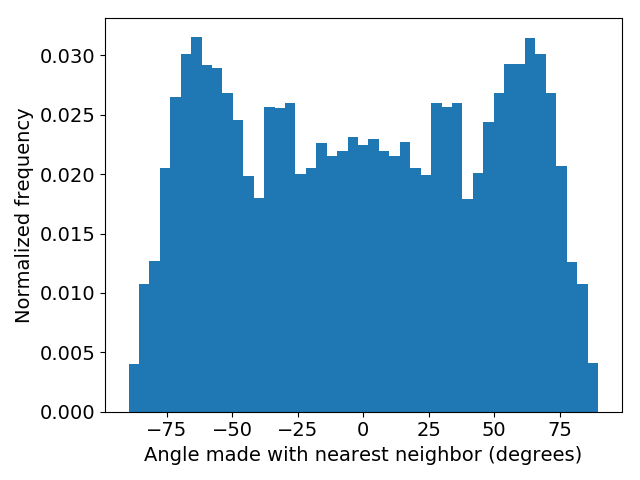
\includegraphics[width=\linewidth]{angles_traj_layered.png}
%		        \caption{}~\label{fig:layered_tails}
%		\end{subfigure}
%		\begin{subfigure}{0.45\textwidth}
%        	\centering
%		        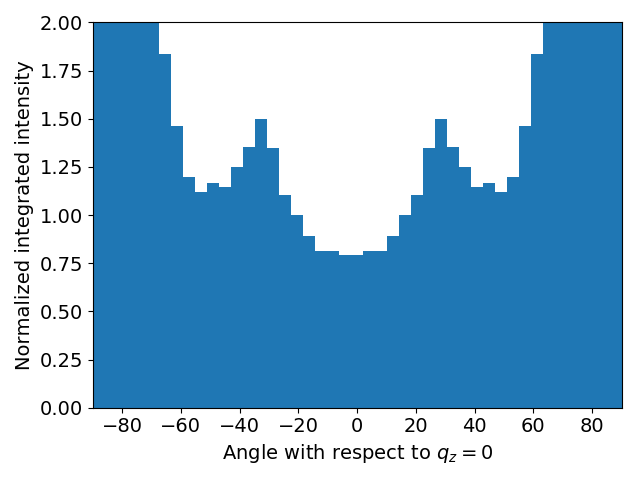
\includegraphics[width=\linewidth]{layered_angle_v_I.png}
%		        \caption{}~\label{fig:layered_integration}
%		\end{subfigure}
%	\end{subfigure} 
%    %MRS4: caption is probably too long.
%    \caption{We hypothesize that R-spots is the result of ordered tail packing.
%	  Defining the membrane plane to be 0\degree, we measured the angles between each
%	  alkane chain tail centroid and its nearest neighbor centroids for the
%	  equilibrated parallel displaced (a) and sandwiched (c) configurations. Peaks
%	  that appear in each distribution are centered near $\pm~33\degree$. We radially
%	  integrated the simulated XRD patterns of the parallel displaced and sandwiched
%	  configuration within the region bounding R-alkanes ((b) and (d) respectively).
%	  Peaks appear in the same location as the angle distributions which corroborates
%	  our hypothesis. Further, we note that the peaks are strongest in both plots
%	  associated with the sandwiched configuration. As shown in Figure
%	  \ref{fig:rz_layered}, systems simulated in the sandwiched configuration exhibit
%	  more intense R-spots reflections. Note that plots of integrated intensity are
%	  normalized so the average alkane intensity (excluding reflections $\pm
%	  30\degree$ from the $q_z$ axis) is set to 1.  Plots are cut off for intensities
%	  greater than 2 so peaks are more visible.}~\label{fig:tail_packing}
%  \end{figure}   		

  % BJC4: modification of above figure to only included sandwiched data. The rest can go
  % in supporting info.
  \begin{figure}[!htb]
  \centering
	\begin{subfigure}{\linewidth}
	\centering
		\begin{subfigure}{0.45\textwidth}
	        \centering
		        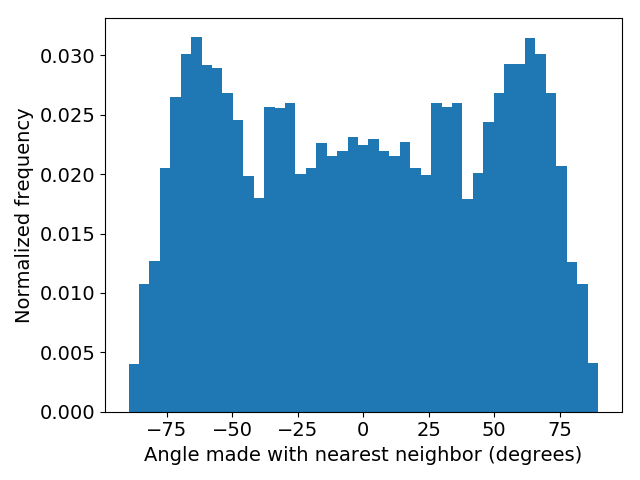
\includegraphics[width=\linewidth]{angles_traj_layered.png}
		        \caption{}~\label{fig:layered_tails}
		\end{subfigure}
		\begin{subfigure}{0.45\textwidth}
        	\centering
		        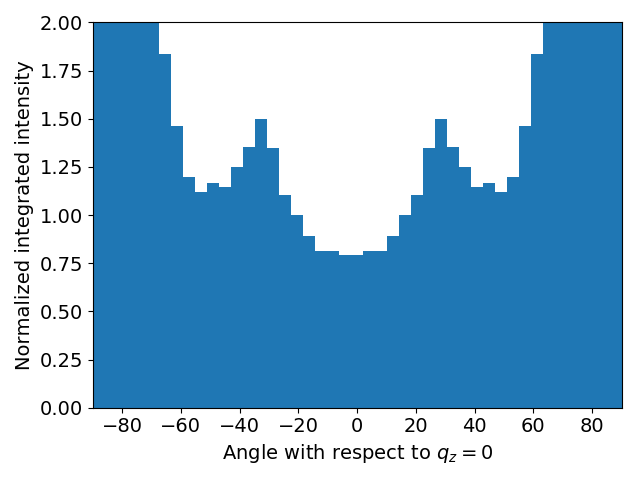
\includegraphics[width=\linewidth]{layered_angle_v_I.png}
		        \caption{}~\label{fig:layered_integration}
		\end{subfigure}
	\end{subfigure} 
    \caption{We hypothesize that R-spots is the result of ordered tail packing.
	  Defining the membrane plane to be 0\degree, we measured the angles between each
	  alkane chain tail centroid and its nearest neighbor centroids for the
	  equilibrated sandwiched configuration simulated at 280K. Peaks
	  that appear in each distribution are centered near $\pm~33\degree$. We radially
	  integrated the simulated XRD patterns of the parallel displaced and sandwiched
	  configuration within the region bounding R-alkanes.
	  Peaks appear in the same location as the angle distributions which corroborates
	  our hypothesis.}~\label{fig:tail_packing}
  \end{figure}  
  
  There are a couple reasons why we see stronger ordered chain packing at 280 K compared to
  experimental conditions of 300 K.
  \begin{enumerate}
  		\item The difference between 280K and 300K is small. Our forcefield parameters
  		may not correctly model the behavior of the tails at 300K (citation?).
  		\item Monomers aren't as confined at 300 K in our simulations versus experiment.
  		If the head groups packed 3.7 \AA apart, the tails would be more confined and forced
  		to pack between vertically adjacent monomer tails. In our case, the tail region is
  		less dense than experiment which gives the tails freedom to organize in a more
  		entropically favored disordered state. 
  \end{enumerate}

% BJC3 : old outline
% R-spots, which appears in both simulated XRD patterns, is a result of the way 
%  alkane tails pack together.
%  \begin{itemize}
%  	\item Previously, the spots in the diffraction pattern had been explained 
%	as the product of tilted alkane chains. % BJC: reference 2014 ACS nano paper
%	\item We measured the tilt angle of the alkane chains and showed that our 
%	system equilibrates to an average tilt angle close to zero degrees ~\ref{fig:tilt} % Could belong in supplemental. Leaving here for now 
%	\item To understand the origin of the spots, we determined which atoms gave rise to the feature
%	\item Since R-spots is present as higher intensity spots within R-alkanes, it is likely
%        that the spots arise as a consequence of the tails. 
%	\item By removing atoms from the trajectory and simulating a diffraction 
%	pattern, we were able to isolate the cause of the spots to the tails (Figure~\ref{fig:tails}).
%	\item Since the tails stay nearly flat, we plotted the centroids of the 
%	tails and measured the angle between each centroid and its nearest neighbors
%	with respect to the plane of the membrane (Figure~\ref{fig:centroids}).  %BJC: at one point Matt mention doing a correlation function instead of just measuring the angles
%	\item We see distinct peaks in the distribution of these angles (Figure~\ref{fig:tail_packing})
%  \end{itemize}
%
%  \begin{figure}
%  \centering
%  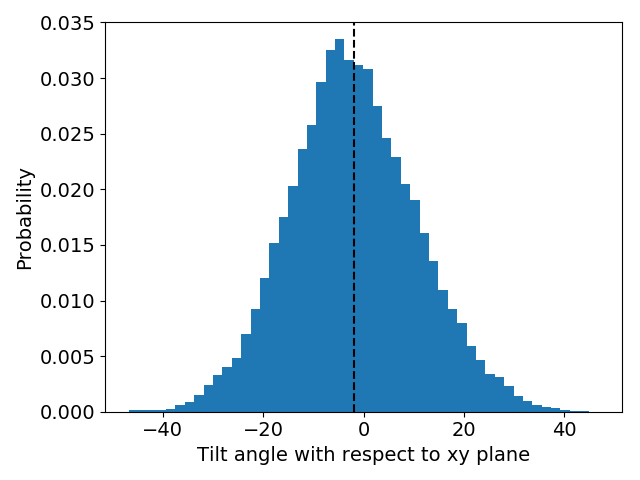
\includegraphics[width=0.5\linewidth]{tilt_dist.png}
%  \caption{The tilt angle distribution of alkane chain tails with respect to the membrane plane
%  indicates an average tilt angle near 7\degree which is far from the 37\degree tilt angle 
%  previously used to explain R-spots}~\label{fig:tilt}
%  \end{figure}
%
%  The peaks in the tilt angle distribution are consistent with the location of R-spots.
%  \begin{itemize}
%	\item The peaks of interest in Figures~\ref{fig:offset_tails}~and~\ref{fig:layered_tails}
%	are located at $\pm$ 33 $\degree$ which is the same location where the highest intensity
%	of spots are located on the simulated patterns
%	\item We confirmed this conclusion by radially integrating the 2D WAXS pattern for q values
%	between 1.57 and 1.4 (real space between 4 and 4.5 \AA) 
%	\item We observe that distinct peaks appear c.a. 30 $\degree$, in close agreement with the
%	previously measured angle distribution (~\ref{fig:offset_integration}~\ref{fig:layered_integration})
%%	\item We integrated the raw experimental 2D WAXS data in the region bounding R-alkanes 
%	\item We performed the same integration on the raw experimental data and found the angle
%	at which R-spots reaches its highest intensity to be $\pm$ 37 $\degree$ which is a 
%	reconcilable difference with our simulated results.  
%  \end{itemize}
%
%  \begin{figure}
%	\centering
%	\begin{subfigure}{0.45\linewidth}
%		\centering
%		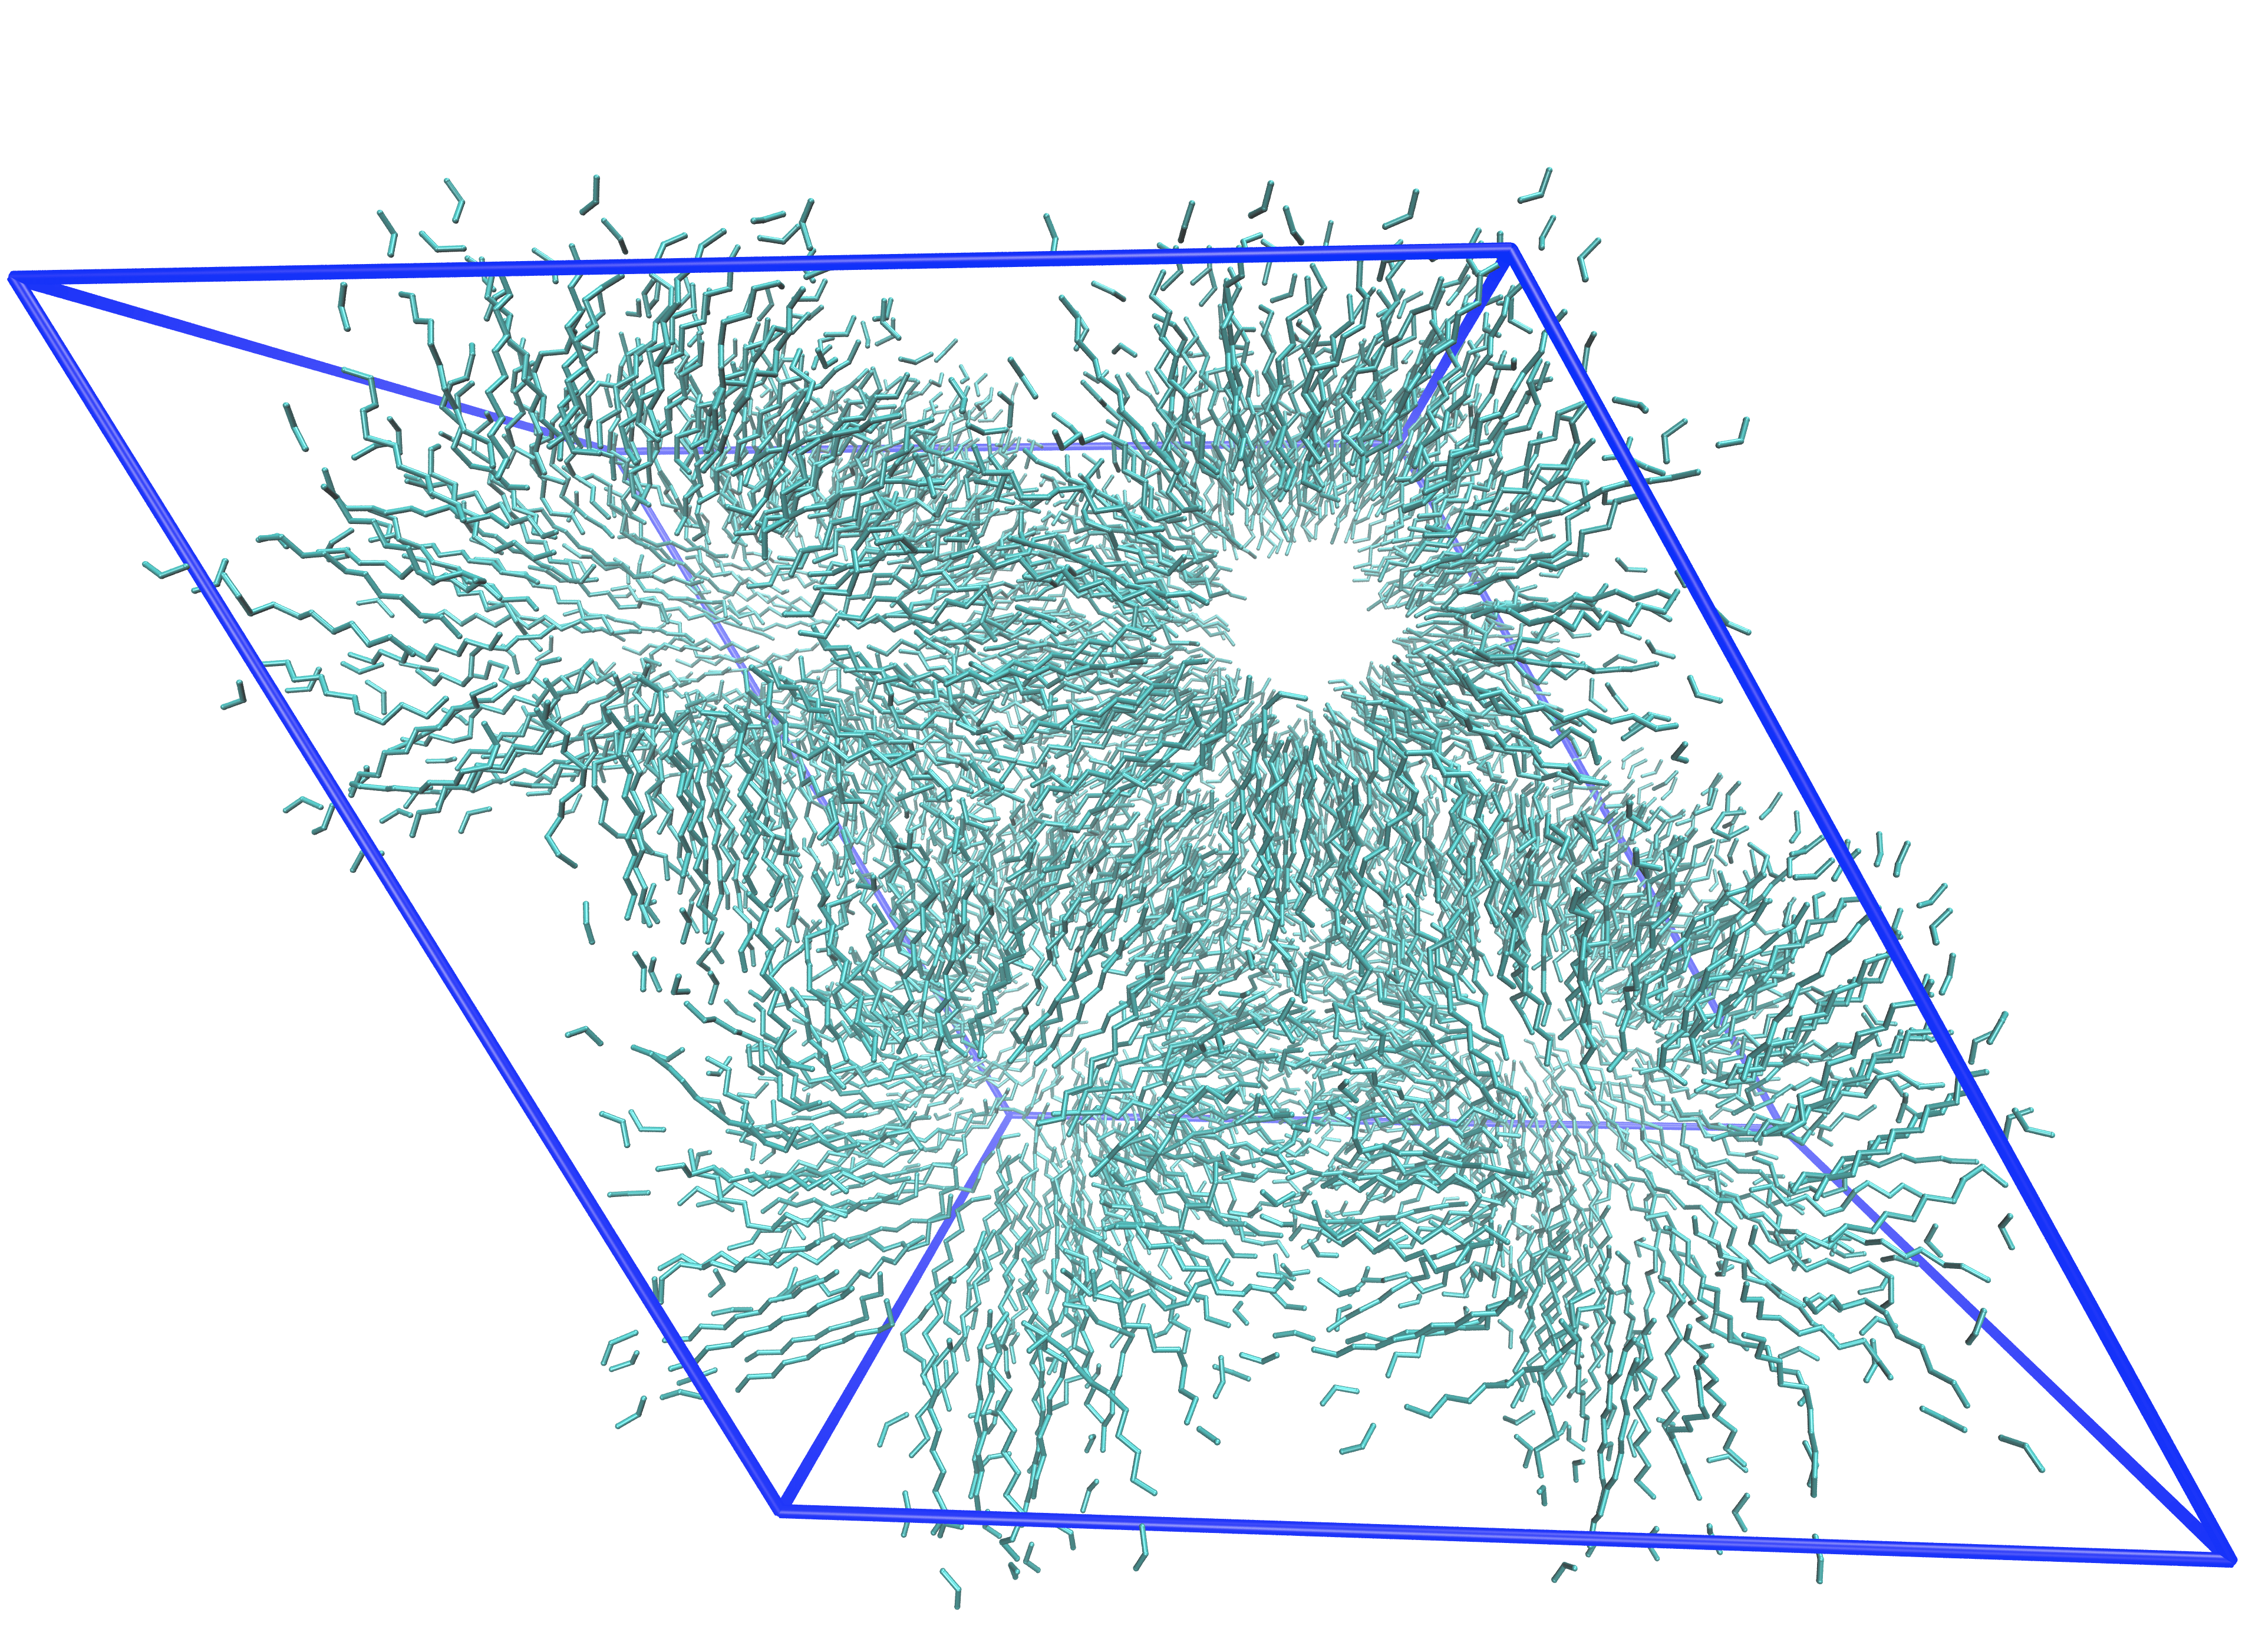
\includegraphics[width=\textwidth]{tails_topview.png}  % picture of top of unit cell with only tail atoms shown
%		\caption{}\label{fig:topdown_tails_only}
%	\end{subfigure}
%	\begin{subfigure}{0.45\linewidth}
%		\centering
%		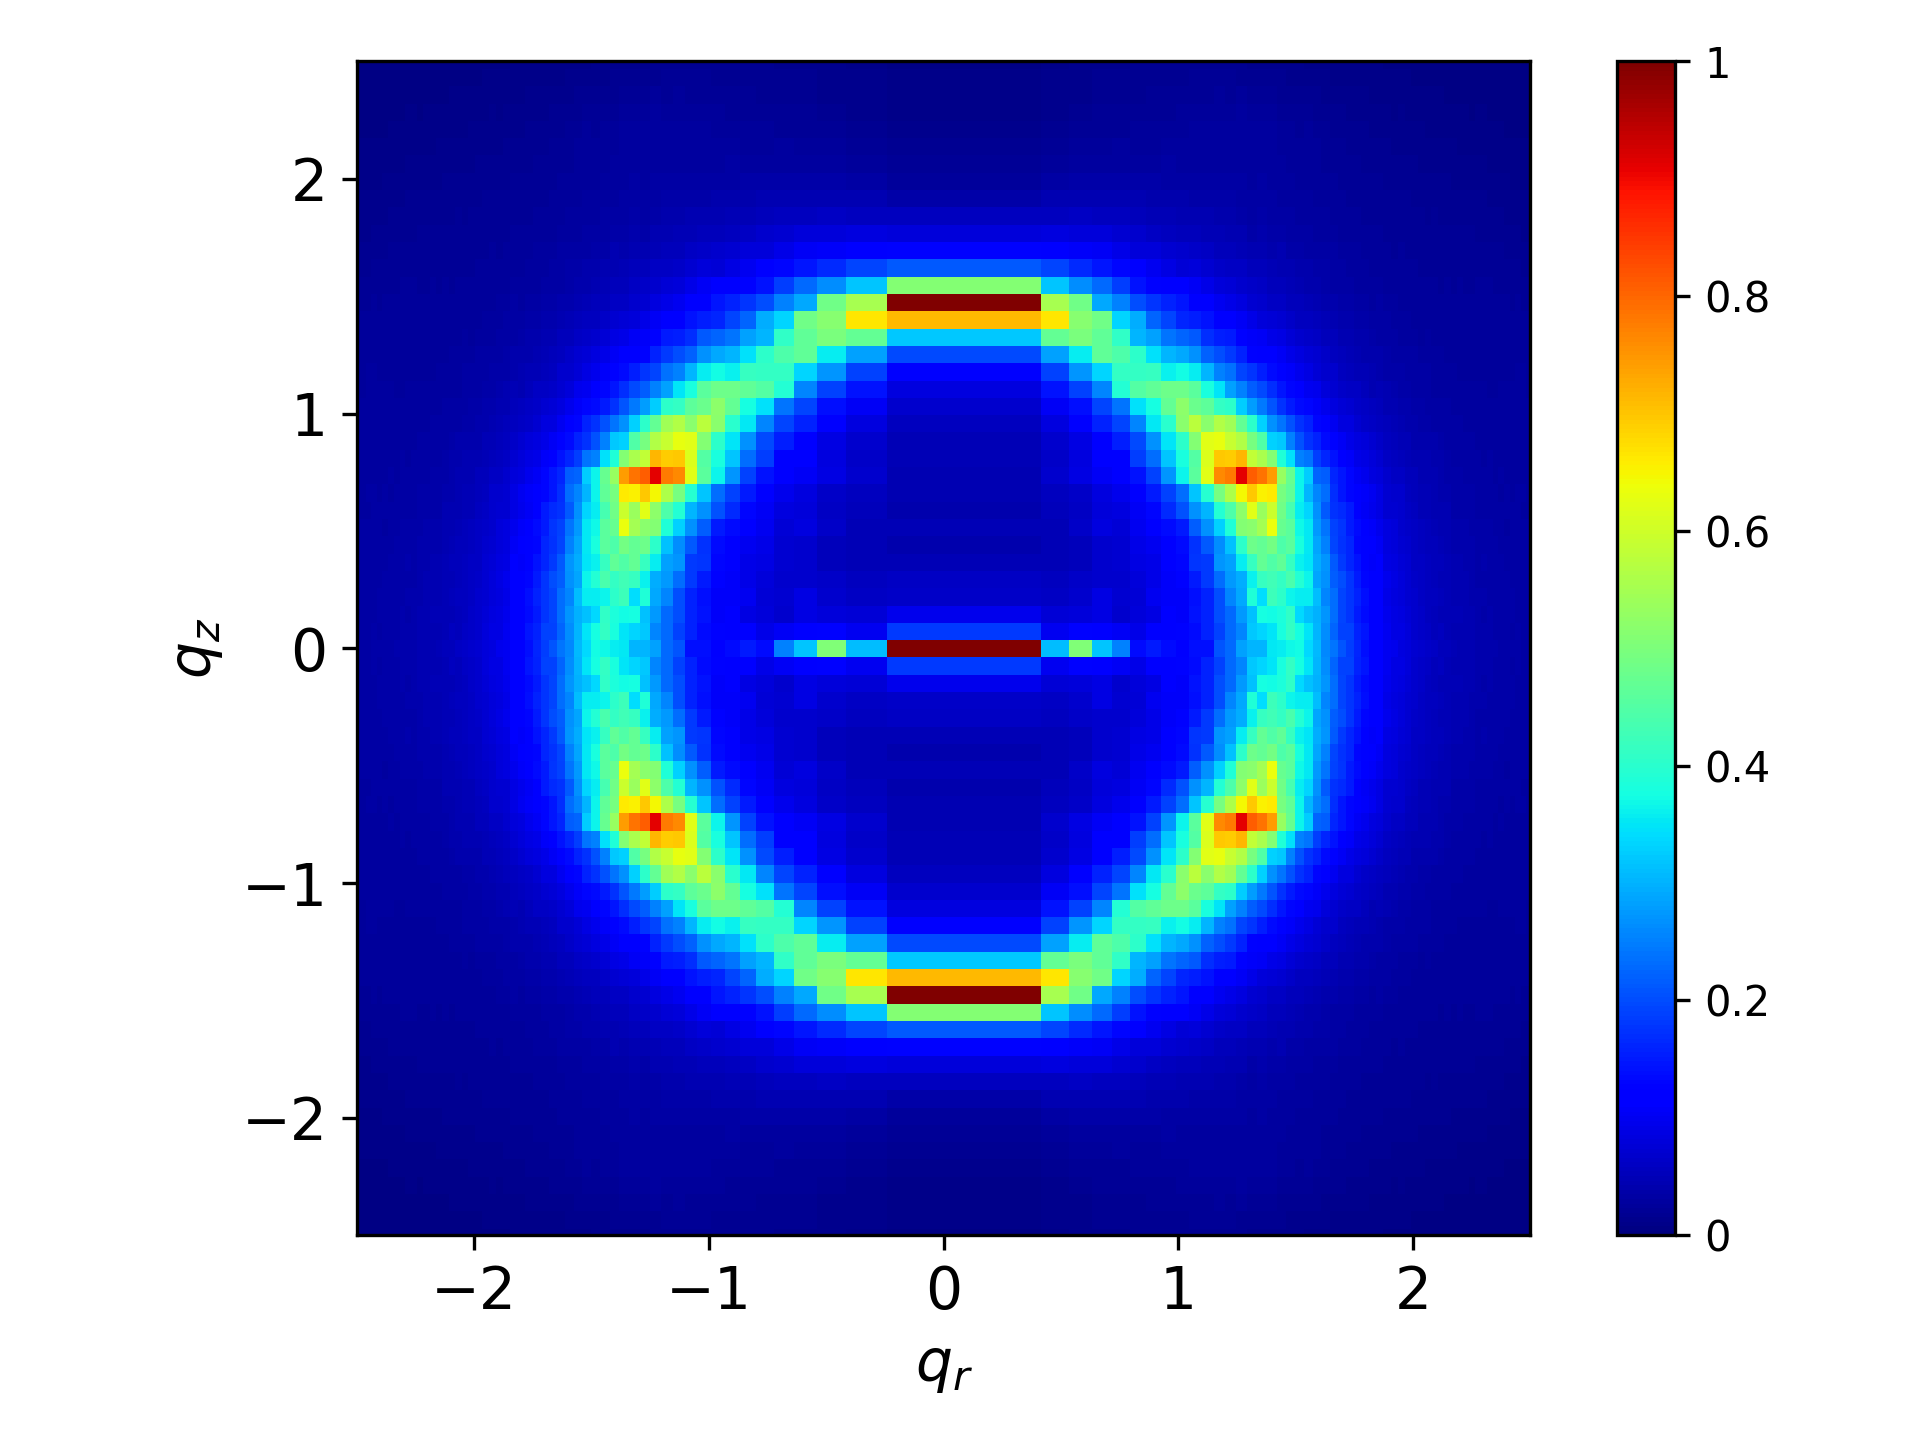
\includegraphics[width=\textwidth]{tails_rzplot.png}
%		\caption{}\label{fig:tails_rzplot}
%	\end{subfigure}
%	\caption{(a) All atoms except carbon atoms making up the tails are removed from the 
%	trajectory. (b) The simulated diffraction pattern of the tail-only trajectory still 
%        shows R-spots}\label{fig:tails}
%        %MRS2: might need to say how the dynamic range is adjusted here with only tails, since otherwise people will be confused with the R-spots being more intense. 
%	%BJC: what do you mean by dynamic range?
%	%BJC: Explain how colorbar is adjusted
%  \end{figure}
% 
%
%  \begin{figure}
%  \centering
%  	\begin{subfigure}{\linewidth}
%	\centering
%		\begin{subfigure}{0.45\textwidth}
%        		\centering
%        		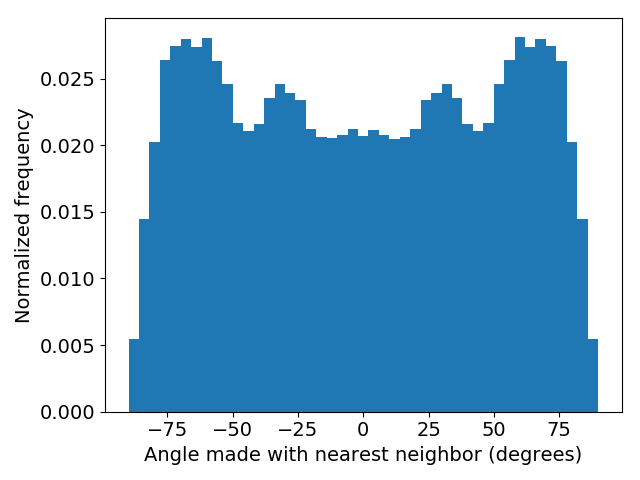
\includegraphics[width=\linewidth]{offset_tail_packing.png}
%        		\caption{}~\label{fig:offset_tails}
%		\end{subfigure}
%		\begin{subfigure}{0.45\textwidth}
%		\centering
%	        	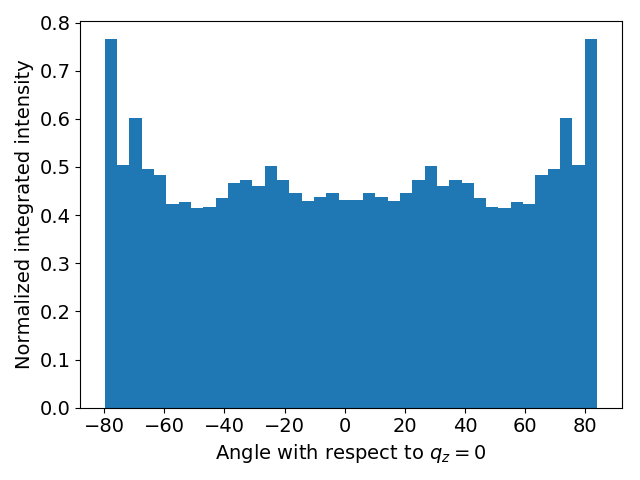
\includegraphics[width=\linewidth]{offset_angle_v_I.png}
%		        \caption{}~\label{fig:offset_integration}
%		\end{subfigure}
%	\end{subfigure}
%	\begin{subfigure}{\linewidth}
%	\centering
%		\begin{subfigure}{0.45\textwidth}
%	        \centering
%		        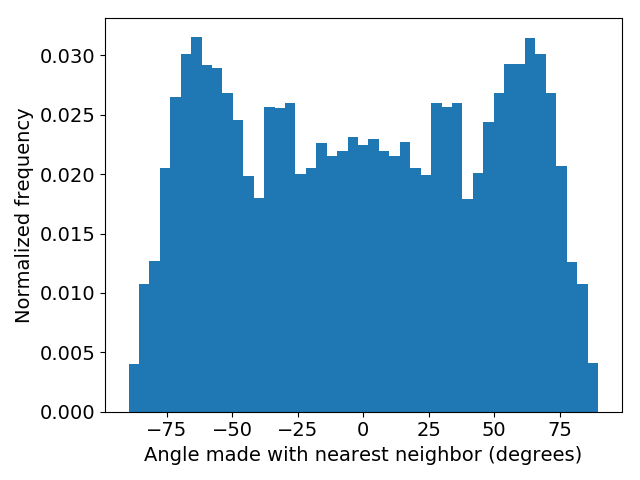
\includegraphics[width=\linewidth]{angles_traj_layered.png}
%		        \caption{}~\label{fig:rz_layered}
%		\end{subfigure}
%		\begin{subfigure}{0.45\textwidth}
%        	\centering
%		        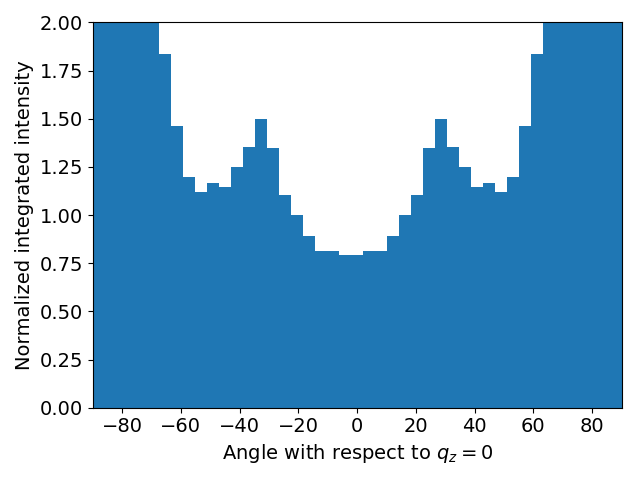
\includegraphics[width=\linewidth]{layered_angle_v_I.png}
%		        \caption{}~\label{fig:layered_integration}
%		\end{subfigure}
%	\end{subfigure}
%%MRS: 
%  \caption{The distribution of angles w.r.t. the xy plane between alkane chain tail centroids and nearest
%  neighbor centroids for equilibrated parallel displaced (a) and sandwiched (c) configurations. The
%  same peaks are visible when the 2D simulated diffraction data is radially integrated in the R-alkanes region,
%  (b) and (d) respectively.}~\label{fig:tail_packing}
%%MRS2: not clear what the difference is between right and left side figures.
%%BJC: That's good! One is angles measured between tail centroids and the other is radial integration of the simulated xrd patterns. I'll try make that more clear in the caption.
%%MRS3: sorry, I meant to say not clear what the SOURCE of the data is in right vs. left.  Make sure colors and labels are consistent in final 
%%MRS: not clear why some are angles with x axis, and some are angles w neighbors?  Shouldn't it be the same thing plotted in both graphs?
%%BJC: I just need to get the labels right, they are the same thing technically
%  \end{figure}

  \subsubsection{Discrepancies between R-$\pi$}\label{section:rpi}
  
  We plotted the one-dimensional pair distribution function, $g(z)$, for the centers
  of mass of monomer phenyl rings (Figure~\ref{fig:correlation}).
  \begin{itemize}
  		\item We averaged all 1D slices in the z-direction of the full 3D correlation function
  		within 2.1 \AA of $(x, y)=(0, 0)$. (full description will be in methods)
  		\item We chose 2.1 \AA as a crude approximation of the radius of the phenyl ring
  		plane. 
  		\item We calculated it as the sum of the longest C-C distance within a phenyl 
  		ring (2.8 \AA) and two times the carbon atom radius (0.7 \AA).
  \end{itemize}
  
  %BJC4: the correlation functions of disordered systems are confusing me.
  \begin{figure}
  \centering
  \begin{subfigure}{0.45\textwidth}
  \centering
  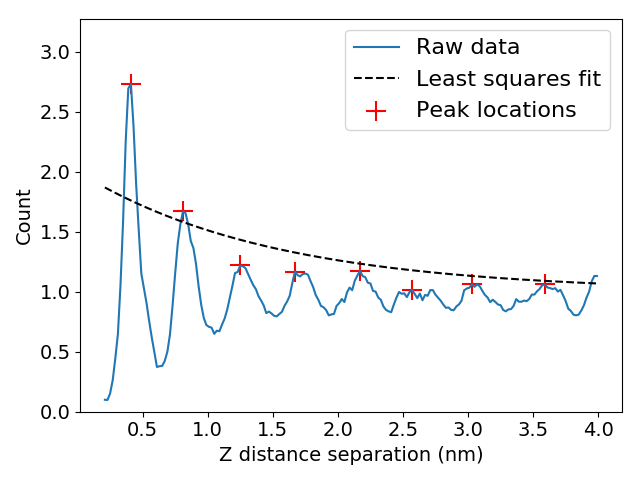
\includegraphics[width=\textwidth]{z_correlation_sandwich.png}
  \caption{}\label{fig:z_correlation_sandwich}
  \end{subfigure}  
  \begin{subfigure}{0.45\textwidth}
  \centering
  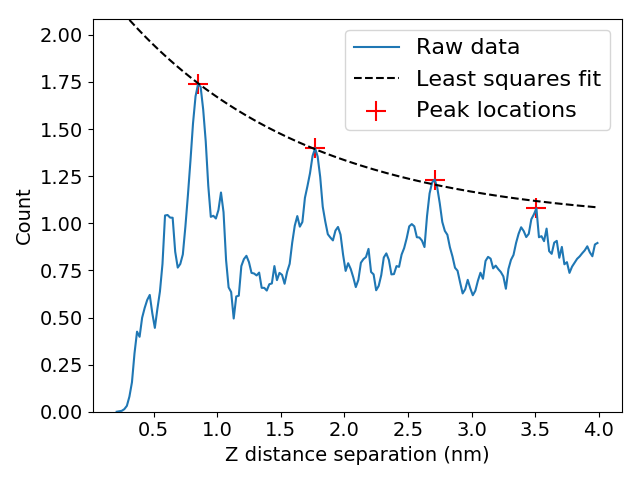
\includegraphics[width=\textwidth]{z_correlation_offset.png}
  \caption{}\label{fig:z_correlation_offset}
  \end{subfigure}  
  \begin{subfigure}{0.45\textwidth}
  \centering
  %BJC4: This is noisier than l=3.7 angstrom, but I can still pick out peaks. I'm unsure
  % how to quantify the difference. The correlation length is very similar to the more
  % ordered configuration.
  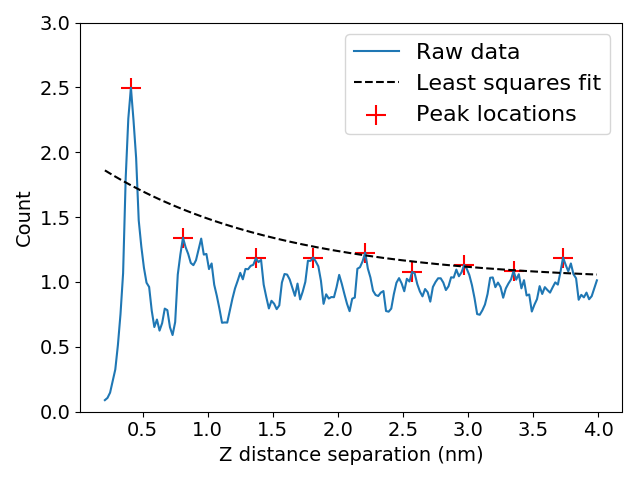
\includegraphics[width=\textwidth]{z_correlation_sandwich_disordered.png}
  \caption{}\label{fig:z_correlation_sandwich_disordered}
  \end{subfigure}  
  \begin{subfigure}{0.45\textwidth}
  \centering
  %BJC4: There really aren't any good peaks here. 
  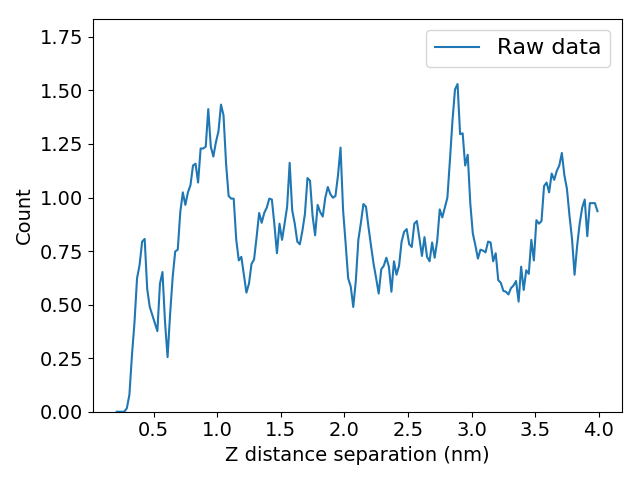
\includegraphics[width=\textwidth]{z_correlation_offset_disordered.png}
  \caption{}\label{fig:z_correlation_offset_disordered}
  \end{subfigure}  
  \caption{}\label{fig:correlation}
  \end{figure}
  
%  The correlation length between stacked monomer head groups shows the best agreement with
%  experimental for systems simulated in the ordered basin.
%  %BJC3: explanation of correlation length calculation in methods section. 
%  \begin{itemize}
%  		\item Correlation length was calculated by fitting a decaying exponential function
%  		to all peaks of $g(z)$ for the sandwiched configuration and to every other peak of
%  		$g(z)$ for the parallel displaced configuration. 
%%  		\item The correlation length of systems simulated at 280K were 27.7 \AA and 25.2 \AA
%%  		for the parallel displaced and sandwiched configurations respectively. 
%  		\item The correlation length of systems simulated in the ordered basin were 11.2 \AA and 
%  		14.9 \AA  		for the parallel displaced and sandwiched configurations respectively. 
%  		\item Systems simulated at 300K show correlation closest to the experimental 
%  		correlation length of 10.1 \AA. They are still slightly more correlated than 
%  		experiment which would lead to an increase in constructive X-ray scattering. 
%  \end{itemize}
  
  The correlation length between stacked monomer head groups shows the best agreement with
  experimental for systems simulated in the ordered basin.
  %BJC4: explanation of correlation function calculation in methods section. 
  %MRS5: the correlation length doesn't look like that great a fit, since it misses the first point by so much.  We may need to reevaluate a litle how this is done. 
  \begin{itemize}
  		\item Correlation length was calculated by fitting a decaying exponential function
  		to all peaks of $g(z)$ for the sandwiched configuration and to every other peak of
  		$g(z)$ for the parallel displaced configuration. 
  		\item The correlation length of systems simulated in the ordered basin were 11.2 \AA and 
  		14.9 \AA  		for the parallel displaced and sandwiched configurations respectively. 
  		\item Something about disordered systems.
  		\item Systems simulated in the ordered basin show correlation closest to the experimental 
  		correlation length of 10.1 \AA. They are still slightly more correlated than 
  		experiment which would lead to an increase in constructive X-ray scattering. 
  \end{itemize}  
  
  Additionally, our system models near-perfectly straight pores with no defects which will
  lead to higher intensity vertical stacking reflections. 
  \begin{itemize}
  		\item Nearly all of the intensity in R-$\pi$ of our simulated patterns is concentrated
  		at a single point. Figure ~\ref{fig:intense_rpi} shows the same simulated patterns with
  		the upper boundary on the colorbar adjusted to be 6x higher. The only distinguishable 
  		reflections are	those of R-$\pi$ and R-pores.
  		\item In the experimental pattern, the intensity is more evenly spread out over all
  		of R-$\pi$. 
  \end{itemize}
  
  \begin{figure}
  \centering
  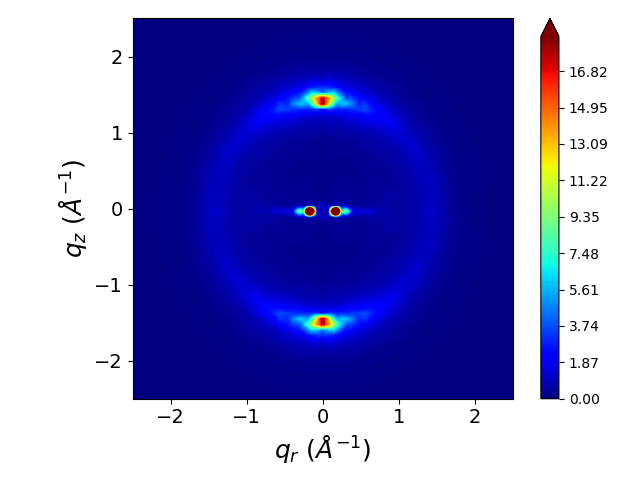
\includegraphics[width=0.4\textwidth]{sandwich_rzplot_highlimit_cbar.png}
  \caption{R-$\pi$ and R-pores are far more intense than the other major reflections. Here, the 
  colorbar was scaled so that the max is 6x higher than all other plots.}\label{fig:intense_rpi}
  \end{figure}
  
  \subsubsection{Origin of R-double}\label{section:rdouble}
  
  R-double will not show up in any of the models tested so far.
  \begin{itemize}
        \item All monomers used to build initial configurations are identical. There is no way 	
        to produce R-double without a more complex initial configuration 
        \item We calculated the structure factor of simple systems that mimic the parallel
        displaced and sandwiched configurations. Neither give rise to R-double.
        (See Figure "fourier transforms of simple systems").
        \item The reflection implies a vertical modulation in electron density every 7.4 \AA.                
        \item This modulation can occur in either the head or the tails
        \item There is a not a unique solution to this problem, however we can speculate based
        on what makes the most physical sense.
  \end{itemize}
  
  We can produce R-double if our initial configuration contains alternating parallel and
  antiparallel carboxylate groups relative to the plane of the monomer's phenyl ring.
  (Figure ~\ref{fig:rotated_carboxylate_rzplot_norestraints}).  
  \begin{itemize}
  		\item It is difficult to physically justify this system. 
  		\item Systems built this way are only stable if position restraints are placed on 
  		all head group heavy atoms. Carboxylate groups quickly revert to the parallel
  		position as restraints are released.
  		\item There is an appreciable energy barrier that prevents rotation
  		of carboxylate groups attached to phenyl rings since the group extends the system's 
  		$\pi$ conjugation. (citation) (See figure in supporting info with energy barrier plots)
  		\item There are instances where carboxylate groups in other systems rotate out of plane.
  		\item Bushey et al. showed that bulky carbonyl-containing substituents of stacked arene
  		molecules tended to tilt 45$\degree$ in order to relieve steric strain, thus allowing 
  		$\pi$-stacking between molecules, and to hydrogen bond with neighboring molecules. 
  		\item Lorenzo and Gra\~{n}a found 3 stable dimers of gallic acid (from which the 
  		monomer, NA-GA3C11 was derived) with adenine. In all cases, the carboxylate group 
  		remained planar, even with evidence of hydrogen bonding between the carboxyl group
  		and nitrogen atoms of adenine. 
  		\item The monomers which we are studying have no opportunities to hydrogen bond and 
  		are confined so that any rotation about the phenyl-carboxylate bond would be sterically
  		hindered. 
  \end{itemize}
  
  We can also produce R-double if layers are not uniformly spaced. Rather, monomers might form 
  pairs that stack less than 3.7 \AA apart, and whose center of masses are spaced 7.4 \AA 
  from the next pair of monomers.(Figure ~\ref{fig:staggered_rzplot_norestraints})
  \begin{itemize}
  		\item To our knowledge, there have been no studies that specifically address the 
  		possibility of a configuration like this. 
  		\item Our forcefield causes our system to tend towards uniformly spaced layers. 
  		\item As expected, simulations of this type of system are only stable if position
  		restraints are applied to heavy atoms of the phenyl rings.
%  		\item Many \textit{ab initio} studies have measured the equilibrium distance between
%  		dimers of benzene and substituted benzene.
%%MRS: don't need to include this point.
%  		\item Tauer and Sherrill explored the binding energies of tetramers of benzene, but
%  		did not explore the report the equilibrium distance between benzene rings. 
%  		\item Even if there have been other studies of the equilibrium distance between 
%  		stacks of benzene rings, it still does not model our system which has many 
%  		electron-withdrawing groups and bulky substituents that would likely affect stacking
%  		preferences. 
  \end{itemize}
  
   Our final hypothesized configuration which produces R-double focus on the orientation of the
   tails. 
   \begin{itemize}
  		\item In this configuration, monomers are rotated so that the vector created by the  
  		bond extending from the carboxylate carbon to the phenyl ring is oriented $\pm 15 	
  		\degree$ with respect to the vector extending from the carboxylate carbon to the pore
  		center (Figure ~\ref{fig:rotated_monomers_rzplot_norestraints})
  		\item Every other monomer layer is rotated $+15 \degree$ and those in between are
  		rotated $-15 \degree$.
  		\item This configuration allows monomer tails to sit between adjacent monomer tails 
  		which may be the most favorable way for them to pack. 
  		\item This configuration is stable short-term while unrestrained.
  		\item This may be the most reasonable explanation for the appearance of R-double. The
  		long-term stability of a configuration similar to this may be feasible if monomers
  		stay stacked 3.7 \AA apart. 
  \end{itemize}
  
  \begin{figure}[htb]
  \centering
  %BJC4: I could cut out the tails in the three real space configurations
  %BJC4: I can remove some of the colorbars and state that they all follow the same color bar. 
  \begin{subfigure}{0.3\linewidth}
  	\centering
  	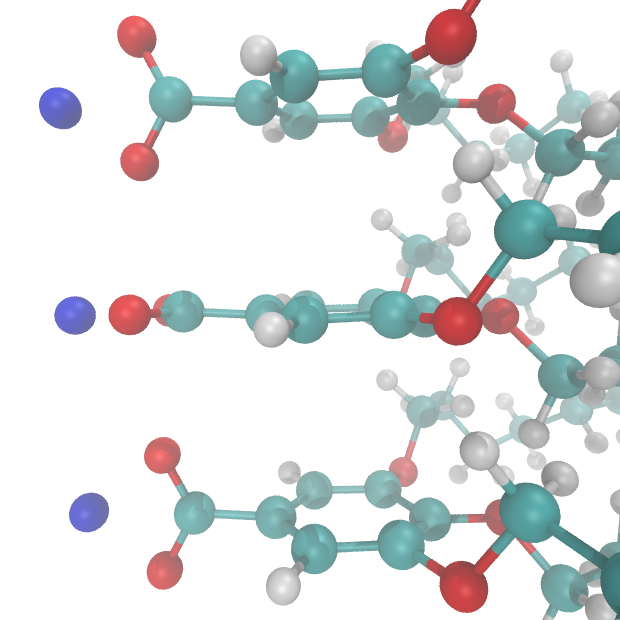
\includegraphics[width=\textwidth]{rotated_carboxylate.png}
	\label{fig:rotated_carboxylate}
  \end{subfigure}
  \begin{subfigure}{0.3\linewidth}
  	\centering
  	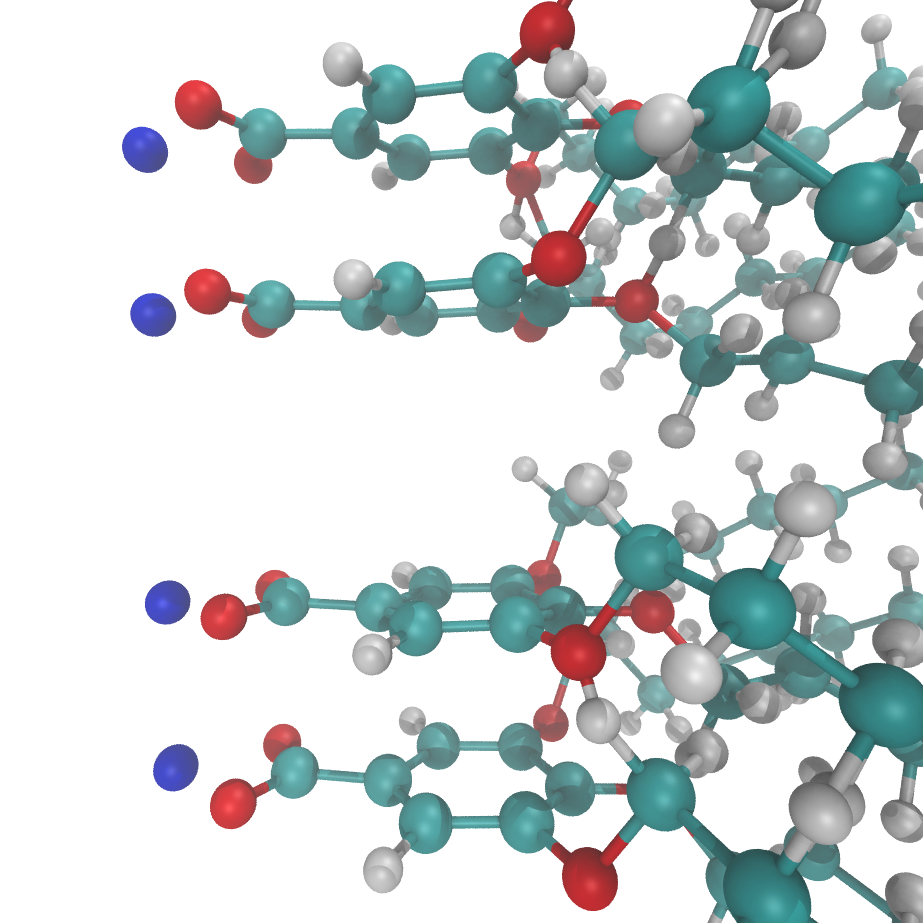
\includegraphics[width=\textwidth]{staggered.png}
	\label{fig:staggered}
  \end{subfigure}
  \begin{subfigure}{0.3\linewidth}
  	\centering
  	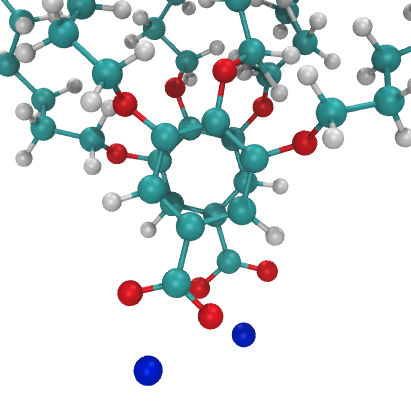
\includegraphics[width=\textwidth]{rotated_monomers.png}
  	\label{fig:rotated_monomers}
  \end{subfigure}
  \begin{subfigure}{0.3\linewidth}
  	\centering
  	\includegraphics[width=\textwidth]{rotated_carboxylate_rzplot_restrained.png}
  	\label{fig:rotated_carboxylate_rzplot_restrained}
  \end{subfigure}
  \begin{subfigure}{0.3\linewidth}
  	\centering
  	\includegraphics[width=\textwidth]{staggered_rzplot_restrained.png}
  	\label{fig:staggered_rzplot_restrained}
  \end{subfigure}
  \begin{subfigure}{0.3\linewidth}
  	\centering
  	\includegraphics[width=\textwidth]{rotated_monomers_rzplot_restrained.png}
  	\label{fig:rotated_monomers_rzplot_restrained}
  \end{subfigure}
  \begin{subfigure}{0.3\linewidth}
  	\centering
  	\includegraphics[width=\textwidth]{rotated_carboxylate_rzplot_norestraints.png}
  	\caption{}\label{fig:rotated_carboxylate_rzplot_norestraints}
  	%BJC4: needs to run longer
  \end{subfigure}
  \begin{subfigure}{0.3\linewidth}
  	\centering
  	\includegraphics[width=\textwidth]{staggered_rzplot_norestraints.png}
  	\caption{}\label{fig:staggered_rzplot_norestraints}
  	%BJC4: needs to be done
  \end{subfigure}
  \begin{subfigure}{0.3\linewidth}
  	\centering
  	\includegraphics[width=\textwidth]{rotated_monomers_rzplot_norestraints.png}
  	\caption{}\label{fig:rotated_monomers_rzplot_norestraints}
  \end{subfigure}
  \caption{R-double is present in all three inital configurations tested while the heavy atoms
  in the headgroup are held in place with position restraints. R-double fades once 
  the position restriants are released.}\label{fig:rdouble}
%MRS5: the conclusion seems like it actually may be ``this doesn't work either''.  How do they line up? Do they go to either parallel displaced or sandwiched?
  \end{figure}
  
  
  %BJC: maybe split into 2 paragraphs
  %MRS2: usually good instinct.  Lead with the conclusions of the research you are trying to convince readers. Rather than phrasing as a question. Something like: ``Layers are well defined and persistent''. 
%  We learned that layers are well-defined and persistent, answering (\ref{point:layers})
  %We verified that the system stays partitioned into layers by
%  We verified our conclusion by
%  plotting the pair correlation function, $g(z)$ calculated between atoms along
%  the length of the pores (Fig~\ref{fig:zdf}).
%  \begin{itemize}
%	\item We measured $g(z)$ with respect to aromatic rings in the head groups
%	and, separately, with respect to carbon atoms on the alkane chains.
	% \item In both cases, we see a degree of layer partitioning
        %\item Using the head groups as reference, we see that sandwiched configuration
%	layers stack 4.29 \angstrom apart while parallel displaced configuration layers
%	stack 4.37 \angstrom apart.
%	\item Using the alkane chain carbons as reference we see a layer spacing of 4.39 \angstrom
%	and 4.38 \angstrom in the sandwiched and parallel displaced configurations respectively.
%        \item The power spectrums used to calculate the reported layer spacings are given in the 
%        Supplemental Information.  %BJC: "Power spectrum" an okay description here?
	% BJC: TODO: Overlay plots of tail and headgroup densities
        %MRS2: repore more precisely what finding is interesting. What does that difference mean?
%	\item We see a difference in the spacing in the head group versus tail region
%	because there is more volume to fill with less densely packed carbon chains in the tail region. 
	% BJC: vvv Need to get the same information for the tail zdfs.
%	\item Even though the layer spacing is similar, the sandwiched configuration
%	exhibits more defined layers with its first peak deviating from the mean 
%        number density by 61 \%. %BJC: I mention how I do this calculation in the methods. Is it clear that I'm doing that here?
%MRS2: fine for description for now.          
%	\item The parallel displaced configuration deviates from the mean by only 
%	12 \% in comparison.
%MRS2: is this that unexpected, since parallel displaces should have layers that alternate anyway?
%BJC: true, but I'm just stating the facts
%  \end{itemize}

%  \begin{figure}
%        \centering
%        \begin{subfigure}{0.45\textwidth}
%                \centering
%                \includegraphics[width=\textwidth]{zdf5layered.png}
%                \caption{}\label{fig:zdf_layered}
%        \end{subfigure}
%        \begin{subfigure}{0.45\textwidth}
%                \centering
%                \includegraphics[width=\textwidth]{zdf5offset.png}
%                \caption{}\label{fig:zdf_offset}
%        \end{subfigure}
%        \caption{Pair distribution functions of aromatic carbons for the
%        (a) 5 monomer per layer, sandwiched and (b) 5 monomer per layer,
%       parallel displaced configurations. Clear periodic maxima in the
%        $z$ probability density indicate distinct layers. The magnitude
%        of the spikes with respect to the average suggest that the 5
%        monomer per layer, sandwiched configuration possesses a higher
%        degree of layer partitioning.}\label{fig:zdf}
%  \end{figure}

  % BJC: Even though I will shift focus to only 5 monomers per layer, I will put other data
  % such as XRD of 4, 6, 7, 8 mon/layer in supplemental information 
  %MRS2: good.
  %\begin{figure}
%	\centering
%	\includegraphics[width=0.5\linewidth]{p2p.png}
%	\caption{The pore spacing (given in nm) of the model increases as
%	number of monomers in each layer increases. The pore spacing of a system
%	starting in the sandwiched configuration is systematically lower than 
%	that started in an offset configuration. Systems built with 5 monomers
%	per layer in a parallel displaced configuration result in a pore spacing
%	closest to the experimental 4.12 nm}~\label{fig:p2p}
 % \end{figure}

  % BJC: This paragraph needs to change since, upon inspection, it appears that the 
  % offset configuration is correct. So it needs to shine a more positive light on offset
  % BJC: I think it can be deleted
  %We varied the initial relative interlayer orientation between sandwiched and 
  %parallel-displaced based on our knowledge of the stability of the two
  %pi-stacking modes.
  %\begin{itemize}
  %	\item We generated simulated X-ray diffraction patterns using simulation 
  %      trajectories from the highly restrained initial configurations created during 
  %	equilibration
  %	\item The simulated patterns establish a difference between the two stacking 
  %	modes (Figure~\ref{fig:XRDrestrained}).
  %	\item In each pattern, R-alkanes is present at a distance of $\approx
  %	1.5$ \angstrom$^-1$ (4.2 \angstrom~ in real space).
  %	\item R-$\pi$ is also present in each pattern, although it appears to 
  %	intersect R-alkanes because the spacing between aromatic rings is 
  %	similar to the alkane chain packing.
  %     %MRS: for above, may need to clarify that this is in simulation, which is different than experiment.
  %	%BJC: okay added some more specific language
  %	\item The difference in aromatic ring spacing between experiment and
  %	simulation is likely a result of the inability of GAFF to properly handle
  %	aromatic interactions. %MRS: provide citations, some mechanistic reasoning.
  %	\item The sandwiched configuration shows R-spots in the expected location.
  %	\item A faint reflection is present in the location of R-double %BJC: but it fades upon further simulation.
  %	\item The parallel displaced configuration contains two lines of high 
  %	intensity with maximum intensity occurring where they intersect the alkane
  %	chain region due to constructive interference between the two features.
  %	\item The lines are located where one would expect to see R-double and, 
  %	perhaps coincidentally, the intersection with R-alkanes occurs where one 
  %	would expect to see R-spots.
	%BJC: might save the following sentence for equilibrium trajectories
  %	\item As the simulation is progressed, the full line begins to fade 
  %	(Figure~\ref{fig:XRDsim}). Most significantly, the line is no longer present
  %	where R-double exists.
  %\end{itemize}

  %\begin{figure}[!ht]
  %	\centering
  %	\begin{subfigure}{0.475\textwidth}
  %		\hspace{-1.2cm}
  %		\centering
  %		\includegraphics[width=\textwidth,valign=t]{rzlayeredrestrained.png}
  %		\caption{}\label{fig:rzplayeredrestrained}
  %	\end{subfigure}
  %	\begin{subfigure}{0.475\textwidth}
  %		\hspace{-1.2cm}
  %		\centering
  %		\includegraphics[width=\textwidth,valign=t]{rzoffsetrestrained.png}
  %		\caption{}\label{fig:rzoffsetrestrained}
  %	\end{subfigure}
  %	\caption{(a) Simulated X-ray diffraction of a sandwiched configuration
  %	with restraints placed on aromatic carbons shows all major features
  %	present in experimental WAXS. Near solid lines at constant z are a result of 
  %	the highly ordered aromatic rings. (b) Simulated X-ray diffraction of a similarly
  %	restrained parallel displaced configuration may also contain all
  %	major experimental WAXS features. One can argue that R-spots is not present
  %	but it is difficult to distinguish because of its intersection with the solid
  %	R-double line. 
        %MRS: Longer simulations are necessary to determine which structure
	% is the best match to experiment
        %MRS: we probably want to avoid saying this (above) if we can.
%}\label{fig:XRDrestrained}
%  \end{figure}

  %MRS: one thought: maybe organize it a different way -- it's not the disordered (and go through the anlysis there), and then separately show that it's more likely the sandwich.  Something to think about.
  %MRS: anyway, this is the key part of the paper, so clarity and organization important.
  %MRS: make sure the figures are comparable.  Could someone look at the figures, and see immediately what you are explaining -- for example, experiment and fully equilibrated disordered, sandwich and parallel displaced all in a row?
  
  %Full comparison of experimental 2D WAXS with simulated X-ray diffraction
  %patterns produced from equilibrated MD trajectories shows the most consistency
  %with the offset configuration in the OP basin.

% BJC: Re-written without mention of basins in follwoing paragraph
 % We answer question (3) by simulating X-ray diffraction patterns produced from
 % equilibrated MD trajectories. We leave open the possibility that the 
 % experimental structure might be reminiscent of the parallel displaced or sandwiched
 % configuration in the OP or CP basin.
  %We created systems using three distinct initial configurations and examined
  %their structure by simulating X-ray diffraction patterns produced from equilibrated MD trajectories.
%  \begin{itemize}
%  	\item OP Basin systems were built in both the parallel displaced and sandwiched 
%	configurations with an intial layer spacing of 3.7 \angstrom~.
%	\item A third system was created by stacking layers in the sandwiched 
%	configuration 5 \angstrom~apart in order to guide it towards the CP Basin.
%	% BJC: I've done an additional offset disordered system which goes to Basin CP but I think that will confuse the point
%	\item The three systems were equilibrated according to our procedure with
%	NPT simulations of greater than 400 ns.
%	\item Simulated diffration patterns were generated using portions of the
%	trajectory after equilibration.  
%	\item We assume the simulation has equilibrated when the distance between 
%	pores and the membrane thickness stopped changing.
%	\item Simulated diffraction patterns for all three structures are shown in 
%	Figure ~\ref{fig:XRDsim}. 
%  \end{itemize}

%  We answer question (\ref{point:orientation}) by simulating X-ray diffraction patterns produced from
%  equilibrated MD trajectories.
  %We created systems using three distinct initial configurations and examined
  %their structure by simulating X-ray diffraction patterns produced from equilibrated MD trajectories.
%  \begin{itemize}
%	\item Systems of 5 monomers per layer in the parallel displaced and sandwiched
%	configurations were tested.
 %       \item Simulated patterns were generated using portions of simulation
  %      trajectory after equilibration.
   %     \item The patterns for both structures are shown and compared to experiment
	%in Figure ~\ref{fig:XRDsim}.
%  \end{itemize}
%

  %BJC: below (commented out) thesis is from when I had the following three paragraphs combined
  %Full comparison of experimental 2D WAXS with simulated X-ray diffraction
  %patterns shows the most consistency with the offset configuration in the OP basin.
  
%  Simulated diffraction of the disordered pore structure in the both the sandwiched
%  and parallel displaced configurations does not match the experimental pattern.
%  \begin{itemize}
%        \item The disordered pore structure exhibits R-alkanes and R-pores but R-double,
%	R-$\pi$ and R-spots are not present. 
%        \item Due to low resolution, making out the individual spots of R-pores is
%        challenging and can be validated with slightly better resolution upon full
%        spherical integration of the 3D structure factor. However, the same
%        information can be extracted by measuring the pore spacing as described earlier.
%        %BJC: ^^^This can be more concise 
%        \item Although the structure's diffraction pattern is very different from
%        experiment, its long-term stability suggests that the structure is realistic.
%	We will explore this further when addressing (4). 
%  \end{itemize}

  %BJC: Put this paragraph first since it is the conclusion I want to stick
%  The parallel displaced configuration results in a simulated XRD pattern with
%  the closest match to experiment.
%  \begin{itemize}
%        \item It produces the only pattern that exhibits all major reflections
%        \item R-alkanes, R-pores and R-$\pi$ appear as they do in the sandwiched configuration.
%        \item R-spots appears, however with a lower intensity relative to R-alkanes
%        when compared to the sandwiched configuration.
%        \item R-double appears apparently due to the parallel displaced aromatic rings
        %BJC: Maybe a figure to explain why this happens
%  \end{itemize}

  %BJC: Put this paragraph second so people understand why it is wrong and don't fixate on how nice the spots are
%  Simulated XRD of the sandwiched configuration contains all experimental features
%  except for R-double.
%  \begin{itemize}
%        \item R-alkanes and R-pores appear in the expected locations.
%        \item R-$\pi$ is also present, intersecting R-alkanes at a lower q value than
%        in experiment. The rings prefer to stack $\approx 4.2 \angstrom$ apart as % update distance if needed
%        opposed to 3.7 \angstrom~.
%        \item Most notably, R-spots appears in the expected location, which suggests 
%        that there is something intrinsic to closer packing that gives rise 
%        to such features. 
%  \end{itemize}

% BJC: Replacement figure below this one
%  \begin{figure}[!ht]
%	\centering
%	\begin{subfigure}{0.31\textwidth}
%		\centering
%		\hspace{-0.9cm}
%		\includegraphics[width=\textwidth]{sandwich_rzplot.png}
%		\caption{}\label{fig:sandwich_rzplot}
%	\end{subfigure}
%	\begin{subfigure}{0.31\textwidth}
%		\centering
%		\hspace{-0.9cm}
%		\includegraphics[width=\textwidth]{offset_rzplot.png}
%		\caption{}\label{fig:offsetrzplot}
%	\end{subfigure}
%	\begin{subfigure}{0.31\textwidth}
%		\centering
%		\hspace{-0.9cm}
%		\includegraphics[width=\textwidth]{disorder_rzplot.png}
%		\caption{}\label{fig:disorder_rzplot.png}
%	\end{subfigure}
%	\caption{(a) All major features except R-double are present in
%	XRD patterns resulting from an equilibrated sandwiched configuration 
%	in Basin A. R-$\pi$ intersescts R-alkanes. R-double faded during equilbration.
%	(b) All major features execpt R-spots are present in XRD patterns 
%	resulting from an equilibrated parallel displaced configuration in Basin A.
%	R-double exists faintly in the expected location. (c) R-pores and R-alkanes
%	are the only major features present in XRD patterns resulting from an 
%	equilibrated disordered phase}\label{fig:XRDsim}
 % \end{figure}

%  \begin{figure}[ht]
%  \begin{subfigure}{.83\linewidth}
%        \centering
%        \begin{subfigure}{0.4\linewidth}
%                \centering
%                \includegraphics[width=\linewidth, trim={2.5cm 0 4cm 2cm}, clip]{WAXS_raw.png}%
%                \caption{}~\label{fig:raw_waxs}
%        \end{subfigure}%
%        \begin{subfigure}{0.4\linewidth}
%                \centering
%                \includegraphics[width=\linewidth, trim={2cm 0 2.5cm 1.25cm}, clip]{rzplot_offset.png}
%                \caption{}~\label{fig:rz_offset}
%        \end{subfigure}
%        \begin{subfigure}{0.4\linewidth}
%                \centering
%                \includegraphics[width=\linewidth, trim={2cm 0 2.5cm 1.25cm}, clip]{rzplot_layered.png}
%                \caption{}~\label{fig:rz_layered}
%        \end{subfigure}%
%        \begin{subfigure}{0.4\linewidth}
%                \centering
%                \includegraphics[width=\linewidth, trim={2cm 0 2.5cm 1.25cm}, clip]{rzplot_disordered.png}
%                \caption{}~\label{fig:rz_disordered}
%        \end{subfigure}
%  \end{subfigure}%
%  \begin{subfigure}{0.14\linewidth}
%        \centering
%        \vspace{-1cm}
%        \includegraphics[width=\linewidth]{colorbar_jet.png}
%  \end{subfigure}
%  \caption{(a) Experimental 2D WAXS data contains 5 major reflections which we aim to match. The remaining
%  three images are diffraction patterns simulated from MD trajectories. (b) The parallel displaced
%  configuration gives rise to all reflections of interest. (c) The sandwiched configurations gives rise to a
%  pattern with all major reflections except R-double. R-spots is strong relative to R-alkanes in comparison
%  to the parallel displaced configuration. (d) The disordered pore configuration creates a pattern with only
%  R-alkanes and R-pores in common with experiment}~\label{fig:xrd}
%  \end{figure}

%  \begin{figure}
%  \begin{subfigure}{0.3\linewidth}
%        \centering
%        \vspace{-0.2em}
%        \includegraphics[width=1.018\linewidth]{layered_rzplot.png}
%        \caption{}~\label{fig:rz_layered}
%  \end{subfigure}
%  \begin{subfigure}{0.3\linewidth}
%        \centering
%        \vspace{0.25em}
%        \includegraphics[scale=0.0987]{WAXS_raw.png}
%        \caption{}~\label{fig:raw_waxs}
%  \end{subfigure}
%  \begin{subfigure}{0.3\linewidth}
%        \centering
%        \includegraphics[width=\linewidth]{offset_rzplot.png}
%        \caption{}~\label{fig:rz_offset}
%  \end{subfigure}
%  \begin{subfigure}{0.0544\linewidth}
%        \centering
%        \vspace{-3.30em}
%        \includegraphics[width=\linewidth]{colorbar_jet.png}
%  \end{subfigure}
%  \caption{The simulated X-ray diffraction patterns for simulations run in the
%  sandwiched (a) and parallel-displaced (c) configurations are compared to experiment (b). 
%  The parallel displaced configuration is the only one that exhibits all major
%  reflections of interest to some degree}
%  \end{figure}

%  The $z$-direction correlation functions show that layers in our model prefer
%  to stack further apart than the 3.7 \angstrom~ suggested by experiment. We attempted equilibration
%  with layers stacked 5.0 nm apart and to our surprise, we observed
%  long-term stability of a qualitatively different configuration suggesting
%  that we have found more than one metastable free energy basin, corroborating \ref{point:metastable}.
%  %that the initial distance between layers can influence the approach towards 
%  %equilibrium.
%  \begin{itemize}
%        \item Equilibrated systems built according to the 3.7 \angstrom~layer spacing
%        implied by R-$\pi$ are characterized by a defined, cylindrical and open pore
%        structure.
%        \item We will refer to this large set of configurations, with an open pore, as
%        the ordered pore basin open pore (Figure~\ref{fig:OPbasin}).
%        \item Simulations of systems built with layers stacked 5
%        \angstrom~ apart results in a pore structure characterized by high radial
%        disorder, while still maintaining partitioning between hydrophobic and
%        hydrophilic regions.
% %MRS3: need to address the similar RDFs.  What data can show they are different? Or maybe they HAVE rdfs, but not good layering? Have you done the fourier transform on them? We can still rule them out based on the XRD, of course.  But surprising the same RDFs.
%        \item This will be called the disordered pore basin (Figure~\ref{fig:DPbasin}).
%        \item This LLC membrane may exist in at least two metastable states.
%        \item The distinct difference in pore structure exhibited by each phase will
%        likely lead to different transport mechanisms.
%        \item Because the pore structure will vary between each basin, understanding
%        which phase exists experimentally is necessary in order to ensure we are
%        studying the system which actually dominates.
%  \end{itemize}

%  \begin{figure}[!ht]
%        \centering
%        \begin{subfigure}[b]{0.475\textwidth}
%                \centering
%                \includegraphics[width=\textwidth]{280K_tramp_close.png}
%                \caption{}\label{fig:OPbasin}
%        \end{subfigure}
%        \begin{subfigure}[b]{0.475\textwidth}
%                \centering
%                \includegraphics[width=\textwidth]{340K_tramp_close_full.png}
%                \caption{}\label{fig:DPbasin}
%        \end{subfigure}
%        \caption{From a qualitative standpoint, the ordered pore basin (a) is characterized by a
%        hollow cylindrical pore while pores in the disorder pore basin (b) are characterized by a
%        higher degree of radial disorder}\label{fig:basins}
%%MRS3: see note on RDF.
%  \end{figure}

  % INSERT XRD of disordered basin
%
%  In order to address \ref{point:poredefinition} and to further understand the structural difference 
%  between the ordered pore and disordered pore basins, we plotted the number of densities of
%  heavy atoms in the head group and tail regions of the monomers in addition to the sodium ions.
%  (See Supplemental Information for definition of head group and tail regions) 
%  \begin{itemize}
%	\item For the hydrophilic region, we used the carbon atoms making up the aromatic ring
%	\item For the hydrophobic components we used all carbon atoms of the monomer tails
%  \end{itemize} 

  % BJC: I'm not sure what to make of this figure right now. The parallel-displaced configuration shares
  % more with the disordered pore phase
  % MRS3: yeah, see my notes on this.  wE need to understand how it can be visually open, and still have this structure.  
  % doesn't this structur have a different pore-to-pore distance.
%  \begin{figure}
%  \centering
%  \begin{subfigure}{0.55\textwidth}
%        \includegraphics[width=1\linewidth]{offset_density.png}
%        \caption{}
%        \label{fig:offset_density}
%  \end{subfigure}
%  \begin{subfigure}{0.55\textwidth}
%        \includegraphics[width=1\linewidth]{layered_density.png}
%        \caption{}
%        \label{fig:offset_density}
%  \end{subfigure}
%  \begin{subfigure}{0.55\textwidth}
%        \includegraphics[width=1\linewidth]{disordered_density.png}
%        \caption{}
%        \label{fig:offset_density}
%  \end{subfigure}
%  \caption{(a) Parallel Displaced (b) Sandwiched (c) ``Disordered''}~\label{fig:densities}
%  \end{figure}
%MRS3: this needs a caption, and need to write some text analyzing it.  The thing that throws me off is that the RDF's look about the same for parallel displaced and disordered!  That's pretty hard to rationalize with the idea that the pores are open vs. closed. What am I missing? Very interesting regardless!

  \subsection{Pore composition}
  
%MRS5: put a little more of the rational for looking at this here. Why should they care?
  We plotted the number densities of heavy atoms in the head group, carbon atoms in the tail
  region and all sodium ions (Figure~\ref{fig:densities}). For the head group
  region, we used the carbon atoms making up the aromatic ring. For the tail
  region we used only carbon atoms of the monomer tails (See Supporting
  Information for diagram). We average the histograms over at least 50 ns of
  equilibrated trajectory.
  
  In general, the composition of the pores is similar between all systems. 
  \begin{itemize}
  	\item We believe we can study transport in any of the systems presented here and
  	still extract valuable information.
  	\item We will need to verify that this assumption is true.
  \end{itemize}  
  
  In all cases, the space in the pore region is filled with sodium ions and
  head groups. Systems in the ordered pore basin are less dense in
  the center of the pore. In both the sandwiched and parallel displaced
  configurations, we see the density of head groups and sodium ions fall to less
  than 50\% of its maximum at r = 0 (Fig.~\ref{fig:layered_density}). The
  situation is most pronounced in the sandwiched configuration where the maximum
  head group density occurs 0.44 nm from the pore center. The parallel displaced
  configuration reaches its maximum 0.35 nm from the pore center. In contrast,
  both disordered pore systems show very little difference in density from its
  maximum. This implies a more uniform distribution of head groups within the
  pore center. This is the same conclusion drawn from the plots of $g(x,y)$ 
  (Figure~\ref{fig:xy_correlation}). 

  There is a partition between the hydrophobic and hydrophilic regions, however
  it is a gradient in composition, rather than an abrupt division. The system
  does not confine sodium ions and head groups to just within the pore region.
  Assuming a pore radius of 0.6 nm, we see in all cases, that 19\% of sodium ions
  exist outside the pore region (except sandwiched, ordered pore, where 16\%
  are outside the pore). Additionally, we see that in all cases, about 3\% of the
  plotted tail density is located within the pore region (except sandwiched,
  ordered pore, where 1.5\% are within the pore region). These observations bring
  into question how one should define a pore in these types of systems. One
  usually measures a membrane's pore radius based on the size of a molecule it
  can reject, however it is not clear where the edges of the pores are and what
  size molecule would fit through. We leave these investigations for a future
  study.

  \begin{figure}
  \centering
  \begin{subfigure}{0.47\textwidth}
        \includegraphics[width=1\linewidth]{offset_density.png}
        \caption{Parallel Displaced, Ordered Pore Basin}
        \label{fig:offset_density}
  \end{subfigure}
  \begin{subfigure}{0.47\textwidth}
        \includegraphics[width=1\linewidth]{layered_density.png}
        \caption{Sandwiched, Ordered Pore Basin}
        \label{fig:layered_density}
  \end{subfigure}
  \begin{subfigure}{0.47\textwidth}
        \includegraphics[width=1\linewidth]{disordered_offset_density.png}
        \caption{Parallel Displaced, Disorderd Pore Basin}
        \label{fig:disordered_offset_density}
  \end{subfigure}
  \begin{subfigure}{0.47\textwidth}
        \includegraphics[width=1\linewidth]{disordered_density.png}
        \caption{Sandwiched, Disordered Pore Basin}
        \label{fig:disorder_layered_density}
  \end{subfigure}
  \caption{In all cases, the component radial distribution functions exhibit a
	  composition gradient transitioning from the hydrophilic to the hydrophobic
	  regions. Systems with layers initially spaced 3.7 \AA~apart in the  parallel
	  displaced (a), and sandwiched (b) configurations both show the highest
	  concentrations of ions and head groups away from the pore center. Systems with
	  layers initially spaced 5 \AA~apart (c) and (d), both show the highest
	  concentrations of ions and head groups near the pore center, implying a more
	  uniform, disordered pore.}~\label{fig:densities}
  \end{figure}
  
  \begin{figure}
  \centering
  \begin{subfigure}{0.32\textwidth}
        \includegraphics[width=1\linewidth]{sodium_density.png}
        \caption{Sodium Ions}
        \label{fig:sodium_regional_density}
  \end{subfigure}
  \begin{subfigure}{0.32\textwidth}
        \includegraphics[width=1\linewidth]{head_group_density.png}
        \caption{Head Groups}
        \label{fig:head_groups_regional_density}
  \end{subfigure}
  \begin{subfigure}{0.32\textwidth}
        \includegraphics[width=1\linewidth]{tails_density.png}
        \caption{Tails}
        \label{fig:tails_regional_density}
  \end{subfigure}
  \caption{Alternate figure : In all cases, the component radial distribution functions exhibit a
	  composition gradient transitioning from the hydrophilic to the hydrophobic
	  regions. Systems with layers initially spaced 3.7 \AA~apart in the  parallel
	  displaced (a), and sandwiched (b) configurations both show the highest
	  concentrations of ions and head groups away from the pore center. Systems with
	  layers initially spaced 5 \AA~apart (c) and (d), both show the highest
	  concentrations of ions and head groups near the pore center, implying a more
	  uniform, disordered pore.}~\label{fig:overlaid_densities}
  \end{figure}

  END!!
  
%  We answer (\ref{point:water}) and further support (\ref{point:orientation}) by preparing parallel displaced and
%  sandwiched configurations according to the wet equilibration procedure.
%  \begin{itemize}
%	\item We do not have an experimental measurement of water in the pores
%	\item We tested a range of water concentrations from 0.5 to 5 percent % working on a 0.5 wt % sytstem now just to see
%	\item Our lower bound represents a system with on average 2 water 
%	molecules for each monomer layer.
%	\item Figure ~\ref{fig:solvation} shows results for each configuration.
%%	\item Initially, we decided the number of waters to put in each pore by
%%	estimating the number of hydrogen bonds in which pore entities could participate.
%%	\item In solution, each headgroup has a charge of -1
%%	\item We estimate there to be at least 2 water molecules per layer based 
%%	on various packing configurations and geometric constraints
%%	\item 4 water molecules per layer translates to about 1.6 wt \%
%  \end{itemize}
%
%  \begin{figure}
%	\centering
%	\includegraphics[width=\textwidth]{solvation.png}  % still working on formatting so this is a screenshot of a doctored latex figure
%        %MRS2: include 0% as well? Maybe leave off 5% if not relevant in the end?
%	\label{fig:solvation}
%  \end{figure}
%
%  In all cases, water disrupts structuring of the model.
%  \begin{itemize}
%	\item The plots in Figure ~\ref{fig:solvation} are normalized 
%	to have the same colorbar as the dry systems. 
%	\item The intensity of the reflections decrease when water is 
%	added to the system.
%	\item In systems built with 5 weight percent water, R-$\pi$ and
%	R-spots become nearly indistinguishable from R-alkanes.
%  \end{itemize}

%MRS3: is this point the right ``main'' thesis to make? I thought it was a more simple statement of being interested as to how water affected the structure.  FYI, would be interesting to see the RDF's of the pores with and without water, BUT I think that's not necessary for this paper, that's more a 2nd paper thing.
%MRS3: we didn't really test if water is  needed to obtain the structures; clearly, w/o water it's metastable for a long time.  We don't need the water simulations to prove this.  
%  Water is not needed to obtain and simulate the correct equilibrium 
%  membrane structure.
%  \begin{itemize}
%	\item We note that water absorbed during membrane synthesis may
%        be present in far lower concentrations than those 
%        tested here.
%	\item We do not eliminate the possibility that water is necessary
%        in order to drive self-assembly. Studying the mechanisms of self assembly is
%	beyond the scope of this work.
%	\item However, once the system has formed the Col\textsubscript{h} 
%	phase, adding water only drives disorder in the structure
%	\item In the equilibrium configuration, if water exists, it is confined
%	to the pore region where there is no driving force for aggregation of 
%	water molecules. 
%	\item In the case of trace water, water molecules will be too sparse to
%	form a hydrogen bonding network.
%  \end{itemize}

  %BJC: old version of above figure v v v
  %\begin{figure}[ht]
  %\centering

  %\begin{subfigure}{0.3\linewidth}
  %      \centering
  %      \includegraphics[width=\linewidth]{offset_tail_packing.png}
  %      \caption{}~\label{fig:offset_tails}
  %\end{subfigure}
  %\begin{subfigure}{0.3\linewidth}
  %      \centering
  %      \includegraphics[width=\linewidth]{angles_traj_layered.png}
  %      \caption{}~\label{fig:layered_tails}
  %\end{subfigure}
  %\begin{subfigure}{0.3\linewidth}
  %      \centering
  %      \includegraphics[width=\linewidth]{integrated_WAXS_ring.png}
  %      \caption{}~\label{fig:rz_layered}
  %\end{subfigure}
  %\caption{The distribution of angles w.r.t. xy plane between alkane chain tail centroids and nearest
  %neighbor centroids for equilibrated parallel displaced (a) and sandwiched (b) configurations both show
  %distinct peaks at $\pm$ 33 $\degree$. (c) Integrated 2D WAXS data between $q_r$=1 and $q_r$=1.42 shows
  %distinct peaks at with maxima at $\pm$ 37 $\degree$}~\label{fig:tail_packing}
  %\end{figure}
 
%BJC: basin stuff that won't be included in this paper
%  The disordered basin shares little in common with the ordered basin but 
%  its long term stability suggests that it can exist under some conditions.  
%  We observed that Basin B is the dominant configuration at higher temperatures.
%  \begin{itemize}
%        \item We linearly ramped the temperature of a system in Basin A
%        from 280K to 340K (just below the experimental isotropic transition temperature) over 100 ns.
%        \item Visually, there is a distinct change in pore structure from one
%        characteristic of the OP Basin (Figure~\ref{fig:280K_pore}) to one characteristic of
%        the CP Basin (Figure~\ref{fig:340K_pore}).
%        \item The slope of all order parameters changes between 315K and 325K
%        (\Cref{fig:p2p_tramp,fig:thickness_tramp,fig:order_tramp}) indicating the
%        possibility of an abrupt change in system ordering.
%        \item Our 100 ns temperature ramp was likely too fast and caused the system
%        to suffer from hysteresis.
%  \end{itemize}

%  We can not immediately classify the OP Basin and the CP Basin as separate phases.
%  \begin{itemize}
%	\item To prove the existence of two phases we need evidence of a
%	a first order phase transition.
%	\item A first order phase transition can be denoted by a discontinuity
%        of some order parameter in response to an external condition such as
%	temperature.
%	\item We chose three easily measurable order parameters: the distance
%	between pores, the membrane thickness and the ratio of pore radius to
%	the uncertainty in pore radius.  % BJC: these may change
%        \item The pore radius is divided by its uncertainty as a way of quantifying
%        the degree to which monomers obstruct the pore region.
%  \end{itemize}

% In an attempt to mitigate hysteresis, we performed slow, stepwise temperature ramps
%  on a parallel displaced and a sandwiched configuration previously equilibrated at 300K.
%  \begin{itemize}
%        \item Every 200 ns, the temperature was raised 5K until we reached 345K
%	\item We performed the same procedure with a system equilibrated in the CP Basin
%	and used it as a benchmark for comparison. 
%  \end{itemize}
%
%  \begin{figure}[!ht]
%        \centering
%        \begin{subfigure}[b]{0.475\textwidth}
%                \centering
%                \includegraphics[width=\textwidth]{280K_tramp_close.png}
%                \caption{}\label{fig:280K_pore}
%        \end{subfigure}
%        \begin{subfigure}[b]{0.475\textwidth}
%                \centering
%                \includegraphics[width=\textwidth]{340K_tramp_close_full.png}
%                \caption{}\label{fig:340K_pore}
%        \end{subfigure}
%        \vskip\baselineskip
%        \begin{subfigure}[b]{0.325\textwidth}
%                \centering
%                \includegraphics[width=\textwidth]{p2p_tramp.png}
%                \caption{}\label{fig:p2p_tramp}
%        \end{subfigure}
%        \begin{subfigure}[b]{0.325\textwidth}
%                \centering
%                \includegraphics[width=\textwidth]{thickness_tramp.png}
%
%                \caption{}\label{fig:thickness_tramp}
%        \end{subfigure}
%        \begin{subfigure}[b]{0.325\textwidth}
%                \centering
%                \includegraphics[width=\textwidth]{order_tramp.png}
%                \caption{}\label{fig:order_tramp}
%        \end{subfigure}
%        \caption{(a) The open pore structure exhibited by a structure equilibrated
%        at 280K is characteristic of the OP Basin. (b) The closed pore structure with
%        a high degree of radial disorder exhibited when the structure in (a) is
%        heated to 340K is characteristic of the CP Basin. (c) A plot of distance between pores
%        vs. temperature changes slope near 325K. (d) A plot of membrane thickness vs.
%        temperature changes slope near 325K. (e) The plot of the ratio of pore radius to
%        its uncertainty changes slope near 315K.}\label{fig:tramp}
%  \end{figure}

%  The CP and OP basins are two configurationally metastable basins.
%  \begin{itemize}
%        \item There is litle change in CP basin properties during the 
%        temperature ramp.
%	\item We observed smooth changes in order parameters as temperature
%        of the OP Basin system was increased implying that we cannot claim the
%	existence of two phases (Figure~\ref{fig:phase_transition}).
%	\item Qualitatively, the pore structure of the OP basin system becomes
%        comparable to one characteristic of the CP basin as temperature is raised. (\Cref{fig:BasinA_280K_pore,fig:BasinB_340K_pore})
%	\item The OP basin system does not converge to the same order parameter
%	values as the CP basin, however it is trending towards Basin B values. (\Cref{fig:p2p_step,fig:thickness_step,fig:order_step})
%	\item To resolve the quanitative discrepancy, we would need a slower 
%	temperature ramp
%	\item Since there are no abrupt changes in any order parameter along the 
%	trajectory, we can conclude that the two basins are not separate phases
%	\item The OP basin is the closest match to what is seen experimentally
%	\item The CP basin is likely an intermediate between the Col\textsubscript{h} 
%	phase and isotropic phase
%	\item The CP basin is present in our simulations at lower temperatures 
%        %MRS: lower temperatures than experiment.  Though nobody has really done the experiments.  
%        %MRS: can we conclude anything from some of the in-situ temperature measurements done by Xunda?  We talked about them, but I don't know they are referenced here.
%	%BJC: Not with what we have because it's in-situ SAXS data which only shows the pore spacing
%	than experiment because our model lacks sufficient $\pi$-$\pi$ iteractions necessary to 
%	stabilize the system into the OP basin. 
%  \end{itemize} 
%
%  \begin{figure}[!ht]
%        \centering
%	% BJC: I'll get actual pictures of the system here. I'm not sure how 
%	% necessary this figure is though. It could go in the supplemental 
%	% information and I can reference the pictures in the previous figure
%	% since they show basically the same idea : Ordered vs. disordered pore
%	% Alternatively, I could show two diffraction patterns here from the 
%	% beginning and end temperature 
%        \begin{subfigure}[b]{0.475\textwidth}
%                \centering
%                \includegraphics[width=\textwidth]{280K_tramp_close.png}
%                \caption{}\label{fig:BasinA_280K_pore}
%        \end{subfigure}
%        \begin{subfigure}[b]{0.475\textwidth}
%                \centering
%                \includegraphics[width=\textwidth]{340K_tramp_close_full.png}
%                \caption{}\label{fig:BasinB_340K_pore}
%        \end{subfigure}
%	\vskip\baselineskip
%        \begin{subfigure}[b]{0.325\textwidth}
%                \centering
%                \includegraphics[width=\textwidth]{p2p_layered.png}
%                \caption{}\label{fig:p2p_step}
%        \end{subfigure}
%        \begin{subfigure}[b]{0.325\textwidth}
%                \centering
%                \includegraphics[width=\textwidth]{thickness_layered.png}
%
%                \caption{}\label{fig:thickness_step}
%        \end{subfigure}
%        \begin{subfigure}[b]{0.325\textwidth}
%                \centering
%                \includegraphics[width=\textwidth]{order_layered.png}
%                \caption{}\label{fig:order_step}
%        \end{subfigure}
%
%	\caption{In all cases, blue lines represent the measured value of
%	the order parameter, black lines are average values calculated from
%	equilibrated Basin B systems at each temperature, green shaded regions
%	represent the standard deviation of each of the black line values, and 
%	red dashed lines show where the temperature is bumped to the next level.
%	(a) At 280K, the system is in a configuration reminiscent of
%	Basin A. (b) At 335K, the system resembles a Basin B configuration. (c) The pore
%	spacing of Basin A decreases with temperature approaching the value 
%	exhibited by Basin B. (d) The thickness of Basin A increases smoothly with 
%	temperature but is far from the Basin B value. Longer equilibrations at 
%	each temperature are needed to allow the system to fully expand. 
%        (e) The ratio of pore radius to uncertainty for Basin A changes smoothly with temperature,
%	converging to a value below that exhibited by Basin B.}\label{fig:phase_transition}
%  \end{figure}

  \subsection*{Ionic conductivity calculation}

  We use the equilibrated parallel displaced system to calculate ionic 
  conductivity since its structure is the closest match to experiment.
  The model gives reasonable estimates of ionic conductivity when compared to 
  experiment.
  \begin{itemize}
  	\item Calculated values of ionic conductivity obtained using the Nernst 
	Einstein relation and Collective Diffusion model are compared in 
	Figure~\ref{fig:conductivity}.
	\item The two methods agree with each other within error, although the 
	uncertainty obtained using the Collective Diffusion model is much higher.
	\item Much longer simulations are needed to lower the uncertainty, however it
	is not feasible to do so with a large system.  
	\item For this reason we will likely only use the Nernst Einstein relation
	in future calculations of this type. 
  \end{itemize}

  The calculated values of ionic conductivity are higher than experiment by an
  order of magnitude. 
  \begin{itemize}
	\item One can justify the reason for this result by considering the 
	real system studied experimentally
	\item The ionic conductivity measurement to which we are comparing was done
	on a \SI{80}{\micro\metre} thick film, nearly 10,000 times thicker than 
        our simulated system. 
	\item The thick film likely has defects leading to non-contiguous pores and
	imperfect alignment.
	\item The 2D SAXS pattern shows the small degree of tortuosity present
	in the system (~\ref{fig:2DSAXS})  % BJC: insert 2D SAXS data -- maybe azimuthal distribution
	\item It has been shown that there is a large dependence of Ionic conductivity
	on the alignment of the pores
	\item The ionic conductivity of an unaligned film is 85 times lower than that
	of a nearly aligned film referenced here  % BJC: reproduce figure from 2014
	\item It is not unreasonable that a thin, perfectly aligned film would have 
	a value of ionic conductivity in agreement with our model
  \end{itemize}

  \begin{figure}
  \centering
  \includegraphics[width=0.5\linewidth]{2D-SAXS_cropped.png}
  % BJC: I will add axes with q values if this ends up in the final draft
  % BJC: I'll also see what I can do about all the white speckles
%MRS2: I'm not sure what the point of this figure is?
%BJC: I put it here at some point in case the need arises. It's mainly to show
% that the pores in the real system are somewhat tortuous, in place of showing
% the Azimuthal distribution which is just an integration of this data. I thought
% it'd be clearer that way since but maybe it's not?
%MRS3: state more clearly in the caption why you are showing it. i.e. ``this data shows that pores in the system are somewhat tortuous'', then explain how the figure shows that.
  \caption{The experimental two dimensional SAXS pattern exhibits reflections
  resulting from highly aligned pore regions. A perfectly aligned system 
  would exhibit sharp dots at the same locations of the refelctions shown. 
  An isotropically aligned system the reflections would appear as 
  rings centered about the origin}~\label{fig:2DSAXS}
  \end{figure}

\begin{figure}
        \centering
        \includegraphics[width=0.5\linewidth]{IC_offset.png}
        \caption{Calculated ionic conductivity using the Nernst-Einstein relation
        and Collective Diffusion model agree with error. Both methods give calculated
        values of ionic conductivity an order of magnitude higher than the experimental
        value}
        \label{fig:conductivity}
\end{figure}

%  The CP basin has a higher ionic conductivity than the OP basin.
%  \begin{itemize}
%	\item We hypothesize that conductivity is enhanced in Basin B due to a 
%	higher sodium ion diffusivity.
%	\item Transport of sodium is likely facilitated by the homogeneity of Basin B.
%	Sodium ions have less nearby sites to move to in Basin A.
%	\item There is currently no experimental evidence of this trend. Maybe Xunda will find something
%	\item In both cases, our calculated values for Basin A are higher than the 
%	experimental values, as expected. 
%	\item Some of the discrepancy is likely a result of using an imperfect forcefield. 
%	\item However, the real system, although mostly aligned and straight, has a 
%	distribution of azimuthal angles, meaning that the pores have a degree of 
%	tortuosity which lowers the effective ionic conductivity of the bulk membrane. 
%	\item The ordering from isotropic to mostly aligned mesophases showed an 85 
%	fold increase in ionic conductivity. We would expect additional gains in a 
%	perfectly aligned system.
%  \end{itemize}

%BJC: vvv replaced by bar plot above
%  \begin{table}[h]
%  \centering
%  \begin{tabular}{ccc}
%  \toprule
%  \multicolumn{3}{c}{Calculated Ionic Conductivity \si{\siemens\per\meter}} \\
%  \hline
%  Method & Basin A & Basin B \\
%  \midrule
%  Nernst Einstein & \num{1.23e-4} (0.01) & \num{1.76e-4} (0.02) \\
%  Collective Diffusion & \num{1.40e-4} (0.32) & \num{4.6e-4}(2.4) \\
%  Experiment & \num{1.33e-5} (0.10) & -- \\
%  \bottomrule
%  \end{tabular}
%  \caption{Calculated ionic conductivity using Nernst-Einsten and Collective Diffusion 
%  agree within error. Both methods give calculated values of ionic conductivity which
%  are an order of magnitude higher than experimental values~\label{table:conductivity}}.
%  \end{table}

  %MRS: the next sections maybe should be supporting?
  %MRS: you say ``the distance decreases by 1 A'' but is that true
  %over all of the different structures?
  %BJC: limiting the discussion to the OP basin in the offset configuration 
  %MRS: Maybe show the difference before and after crosslinking in X-ray, to show that you can't tell?
  %MRS: you don't otherwise discuss clearly what effect crosslinking would have. 
  \subsection*{Implementation of the crosslinking algorithm}

  We applied the crosslinking algorithm to the equilibrated parallel-displaced  
  configuration with 5 monomers per layer.
  \begin{itemize}  %BJC: working on the following. The following is what I expect
%  	\item There is an even distribution of crosslinks between same monomer tails, 
%	between monomers in the same pore and between monomers in different pores 
%	including periodic boundaries.  % BJC: might leave this detail in the supplemental
	\item We reach 95 \% conversion of terminal vinyl groups % BJC: we'll see
	\item The distance between pores shrinks by 0.4\angstrom~ after the system is 
	crosslinked  
	\item We simulated the crosslinked system in the NPT ensemble for 100 ns
	\item Major features are still present in the X-ray diffraction, however at lower intensities ~\ref{fig:rzplot_xlink} 
	\item The ionic conductivity is lower in the crosslinked system ~\ref{fig:ic_xlink} % BJC: Nernst-Einstein is lower. Need a longer simulation to check Collective-Diffusion - I can probably avoid that by saying that we will be sticking with the Nernst-Einstein method
  \end{itemize}
 

  \begin{figure}
  \centering
  \begin{subfigure}{0.45\textwidth}
	\centering
	\includegraphics[width=\textwidth]{rzplot_xlink.png}
	\caption{}~\label{fig:rzplot_xlink}
  \end{subfigure}
  \begin{subfigure}{0.45\textwidth}
	\centering
	\includegraphics[width=\textwidth]{ic_xlink.png}
	\caption{}~\label{fig:ic_xlink}
  \end{subfigure}
  \caption{(a) Reflections produced by the crosslinked configuration fade relative
  to the uncrosslinked system. The colorbar shown is the same used for the uncrosslinked
  system. (b) The ionic conductivity is smaller relative to the uncrosslinked system, but
  still much larger than the experimental value}~\label{fig:xlink}
  \end{figure}
 
%  \begin{figure}
%	\centering
%	\begin{subfigure}{0.31\textwidth}
%		\centering
%		\includegraphics[width=\textwidth]{p2p_diagram.PNG}
%		\caption{}\label{fig:p2p_diagram}
%	\end{subfigure}
%		\begin{subfigure}{0.31\textwidth}
%		\centering
%		\includegraphics[width=\textwidth]{no_xlink_p2p.png}
%		\caption{}\label{fig:no_xlink_p2p}
%	\end{subfigure}
%		\begin{subfigure}{0.31\textwidth}
%		\centering
%		\includegraphics[width=\textwidth]{xlink_p2p.png}
%		\caption{}\label{fig:xlink_p2p}
%	\end{subfigure}
%	\caption{(a) The legends of the plots in (b) and (c) refer to the numbers shown.
%	Each numbered circle represents a pore. Distances are measured along each of the 
%	lines shown in addition to the distance from pore 1 to pore 4. (b) The positions
%	of individual pores fluctuate in an uncrosslinked system. (c) The positions of
%	individual pores in the crosslinked system are stable relative to the uncrosslinked
%	system}\label{fig:xlink}
%  \end{figure}
  
  \section*{Conclusion}
  
  We have used a detailed molecular model of the Col\textsubscript{h} phase formed by NA-GA3C11
  in order to study the nanoscopic structure.
  \begin{itemize}
  	\item While there have been efforts to model formation of various liquid crystalline 
	phases with molecular dynamics, to our knowledge there have been no studies which 
	attempt to examine their structure with the same level of detail presented here.
	\item Evidence strongly supports that layers are composed of 5 monomers
        \item We have confirmed that monomers stay partitioned in layers.
	\item We have explored the affect of two different $\pi$-$\pi$ stacking modes on the equilibrated
	membrane strucure. 
	\item Simulated diffration patterns generated from MD trajectories suggest that
	the parallel-displaced configuration produces a structure with the closest match to experiment.
%MRS3: water is not needed to create well-defined pore structures?  I'm not sure ``maintain'' is the right word, and ``membrane structure'' may be too vague.
	\item Finally, water is not needed to maintain membrane structure our data 
	shows that it actually disorders the pore
	\item Now that we have a good idea of what the membrane structure should look like, we will
	evaluate transport of various solutes within the system. 
         %MRS2: I'd like to see a bit more information about ``pore size'', and the RDF's of the constituents.  What FITS through a pore is another paper.
        \item We will apply the knowledge gained from this study in order to 
        suggest improvements to the existing system as well as to evaluate new
	unsynthesized LLC systems.
%	\item Even though our model only answers these questions for a system created by 
%	NA-GA3C11, it can be adapted to other study systems formed by other LCs with 
%	little extra effort. 
  \end{itemize}
  
\clearpage
\bibliography{llc}

\end{document}
